\documentclass[11pt]{article}
\usepackage[T1]{fontenc}
\usepackage[utf8]{inputenc}
\usepackage{lmodern}
\usepackage[margin=0.78in]{geometry}
\usepackage{microtype}
\usepackage{booktabs,tabularx,array,longtable}
\usepackage[dvipsnames]{xcolor}
\usepackage{graphicx}
\usepackage{enumitem}
\usepackage{hyperref,fancyhdr,titlesec}

\definecolor{navy}{HTML}{17365D}
\definecolor{blue}{HTML}{2F75B5}
\definecolor{teal}{HTML}{218A8D}
\definecolor{green}{HTML}{2E7D32}
\definecolor{amber}{HTML}{A86600}
\definecolor{red}{HTML}{B13A3A}
\definecolor{graytext}{HTML}{4A5560}
\definecolor{lightblue}{HTML}{EAF3F8}
\definecolor{lightteal}{HTML}{EAF6F4}
\definecolor{lightamber}{HTML}{FFF5E2}
\definecolor{lightred}{HTML}{FBECEC}

\hypersetup{colorlinks=true,linkcolor=navy,urlcolor=blue,
  pdftitle={AF--FNO Results Tracker},pdfauthor={AF--FNO project}}
\pagestyle{fancy}\fancyhf{}
\lhead{AF--FNO project}\rhead{Results and decisions}\cfoot{\thepage}
\renewcommand{\headrulewidth}{0.3pt}
\setlength{\headheight}{14pt}
\titleformat{\section}{\Large\bfseries\color{navy}}{\thesection}{0.7em}{}
\titleformat{\subsection}{\large\bfseries\color{blue}}{\thesubsection}{0.7em}{}
\setlist[itemize]{leftmargin=1.35em,itemsep=2pt,topsep=4pt}
\setlength{\parindent}{0pt}
\setlength{\parskip}{5pt}
\renewcommand{\arraystretch}{1.16}
\newcolumntype{Y}{>{\raggedright\arraybackslash}X}
\newcommand{\MITgcm}{\textsc{MITgcm}}
\newcommand{\Pass}{\textcolor{green}{\textbf{Pass}}}
\newcommand{\Fail}{\textcolor{red}{\textbf{Fail}}}
\newcommand{\Active}{\textcolor{blue}{\textbf{Active}}}
\newcommand{\Pending}{\textcolor{amber}{\textbf{Pending}}}
\newcommand{\resultbox}[3]{%
  \begin{center}\setlength{\fboxsep}{8pt}%
  \fcolorbox{#1}{#2}{\begin{minipage}{0.92\textwidth}#3\end{minipage}}%
  \end{center}}
\newcommand{\widefigure}[2]{%
  \begin{center}
  \IfFileExists{#1}{%
    \includegraphics[width=0.96\textwidth]{#1}%
  }{%
    \fcolorbox{amber}{lightamber}{\parbox[c][1.0in][c]{0.90\textwidth}{%
      \centering\textbf{Planned output; not generated}\par
      \small\nolinkurl{#1}}}%
  }\par
  \small\color{graytext}#2
  \end{center}}
\newcommand{\pairedfigures}[4]{%
  \begin{center}
  \begin{minipage}[t]{0.485\textwidth}\centering
    \IfFileExists{#1}{\includegraphics[width=\textwidth]{#1}}{%
      \fcolorbox{amber}{lightamber}{\parbox[c][0.85in][c]{0.88\textwidth}{%
        \centering\textbf{Planned output}\par\scriptsize\nolinkurl{#1}}}}\par
    \small\color{graytext}#2
  \end{minipage}\hfill
  \begin{minipage}[t]{0.485\textwidth}\centering
    \IfFileExists{#3}{\includegraphics[width=\textwidth]{#3}}{%
      \fcolorbox{amber}{lightamber}{\parbox[c][0.85in][c]{0.88\textwidth}{%
        \centering\textbf{Planned output}\par\scriptsize\nolinkurl{#3}}}}\par
    \small\color{graytext}#4
  \end{minipage}
  \end{center}}

\begin{document}

\begin{center}
  {\sffamily\bfseries\color{navy}\fontsize{24}{28}\selectfont
  AF--FNO Results Tracker\par}
  \vspace{0.10in}
  {\large Frozen forward emulators, derivative tests, and scientific decisions\par}
  \vspace{0.12in}
  {\color{graytext}\textbf{Status date: 30 July 2026} \quad
  Protocol: \texttt{AF\_FNO\_Project\_Plan.tex}}
\end{center}

\begingroup\color{graytext}
\textbf{Current scientific decision.}  Keep A0, A, and B frozen as controls.  Model C's
width-32 duration and width-64 capacity tests were scientifically rejected because SSH
did not beat persistence.  A training-only late-checkpoint audit showed that the
increment gradient was already substantial, SSH-dominated, and aligned with the state
gradient, making late optimization stability more plausible than missing capacity.
Bounded job 287583 then showed that a larger increment weight fails, whereas preserving
loss v1 and decaying the learning rate fivefold after epoch 240 passes every 96-record
memorization criterion at epoch 315.

Search contract v1 then completed exactly as frozen in jobs
287604/288466/289379/289915.  It selected \((24,16)\), width 64, four layers, and
10\% padding; neither conditional architecture trigger fired.  Final-seed job 290382
completed cleanly and every checkpoint reloaded exactly, but all three seeds narrowly
missed the strict SSH gate at 1.00014/1.00383/1.03818 times persistence.  U, V, and
temperature beat persistence for every seed.  The immutable decision therefore
scientifically rejects Model C validation-search v1, does not freeze a configuration,
and does not authorize inference.  This is a generalization failure, not an operational
failure.  Inference, intermediate-wind, response, and adjoint data remain sealed while
a separately versioned post-search data-adequacy decision is applied.

GPU job 290415 completed that frozen decision without reading inference.  All four
expansion checks passed, while low-wind S1 SSH remained worse than persistence even on
training.  The authorized expansion is now complete: array 290439 extended all three
regimes normally, jobs 290443/290444 built and independently validated the immutable
11~GB trajectory-v2 store, and training-only job 290446 passed the predeclared
two-times effective-coverage target for temperature and SSH state and increment
proxies.

Fresh v2 validation remains unread.  Contract
\path{config/model_c_successor_training_v1.json}, SHA-256
\texttt{3e0a300e73ec...159285}, freezes an exact width-64 data-only control, an isolated
width-64 \(4C\) Channel-MLP test, and only then a candidate restoring Bire's absolute
width 128 and internal lift, projection, and Channel-MLP ratios.
GPU array 290448 completed both phase-1 candidates normally.  Both pass exact reload
and decorrelation-aware 90/180-day amplitude stability but fail only S1 SSH:
the data-only control scores 1.103435 times persistence, while isolated \(4C\)
channel mixing reduces this to 1.003573 and improves every aggregate group.
Contracted width-128 job 290597 then completed in 1h20m22s and passed every training
criterion at aggregate U/V/temperature/SSH ratios
0.049040/0.121279/0.384816/0.522413; S1 SSH is 0.762683.  Corrected fresh-validation
contract SHA-256 \texttt{56bb6ec59799...0cf27b} is frozen before state metrics.
Split-1 array 290673 completed the two missing replicas, and all three seeds pass every
training/reload/stability criterion at worst regime/group ratios
0.762683/0.732270/0.839507.  Fresh-validation job 290738 nevertheless rejects C:
surface speed passes all baselines, while SST/surface-pressure RMSE-AUC ratios to
persistence are 2.313/2.198 because slow-field error accumulates after days 20--30.
Training-only rollout-diagnosis job 291102 then reproduced the same drift for every
seed on balanced split-1 chronology, classifying an objective/checkpoint-gate mismatch.
A versioned companion to Bire-style Figure~4 now exposes SST and surface-pressure
baselines at readable scale: SST first loses both persistence and climatology at day
20; surface \(P/\rho\) loses persistence at day 30 and climatology at day 70.
Exact-replay job 291164 completed in 1h19m14s and reproduced the original
step-14,880 state dictionary bit for bit, with zero numerical difference in the
six-row training history.  None of the six late checkpoints passes the frozen
10--90-day gate, so the result is
\texttt{objective\_correction\_required}, not a checkpoint-selection fix.  Diagnostic
best step 14,400 retains the old ten-day gate at worst ratio 0.85235, but at day 90
its SST RMSE is 3.669/5.513 times persistence/climatology and surface-\(P/\rho\)
RMSE is 3.800/2.247 times those baselines.

Pushforward job 291612 completed normally in 20m37s.  Its step-1,920 checkpoint is
best by every frozen selection priority and reloads bitwise, but the complete gate
still fails.  Relative to the step-14,400 source, worst primary RMSE-AUC improves
from 2.366 to 1.692, worst slow-field lead ratio from 5.513 to 3.994, and the
ten-day worst regime/group ratio from 0.852 to 0.610.  At day 90 the best SST ratios
are 2.659/3.994 to persistence/climatology and surface-\(P/\rho\) ratios are
3.222/1.905.  The result is a useful directional improvement, not baseline skill;
replication and validation remain unauthorized.

Duration job 291616 completed normally in 51m31s and first reproduced pushforward
step 1,920 bit for bit.  None of its eight checkpoints passes the complete gate.
Diagnostic-best step 5,760 improves worst primary RMSE-AUC to 1.597 and worst
slow-field lead ratio to 3.609, while retaining the old ten-day gate at 0.566.
At day 90, SST is still 2.402/3.609 times persistence/climatology and surface
\(P/\rho\) is 2.922/1.727 times those baselines.  The bounded duration test therefore
rejects undertraining as a sufficient explanation and classifies detached
terminal-only supervision as structurally insufficient.

Corrected truncated-unroll contract v2, SHA-256
\texttt{0c5aabadbe51...92e3c}, froze the predeclared next test.  Job 291769 stopped
before training because its source validator used the wrong checkpoint step-field
name; v2 moved that check into preflight without changing the scientific objective.
Job 291778 then completed normally but failed scientifically.  Its diagnostic-best
step 1,920 reloads a nine-step rollout bitwise, yet worst primary RMSE-AUC/slow-lead
ratios are 1.933/3.701, both worse than duration step 5,760 at 1.597/3.609.
No replica, fresh-validation, or inference job is authorized.  The active conclusion
is now more specific than ``try another temporal objective'': strong velocity and
streamfunction skill, extremely small slow-field persistence error, and large-scale
increment energy make signed slow-tendency drift the first mechanism to test.

Bias/projection job 292064 subsequently showed that fixed signed bias is material but
not dominant, and rollout-conditioned loss-v3 job 292293 improved worst primary AUC
to 1.462 while leaving worst slow-field lead at 3.634.  Pointwise-anomaly/direct-state
job 303447 now supplies the decisive representation result.  It selected step 14,400
using split 1 only and passed the strict training gate at worst primary
AUC/slow-field-lead ratios 0.394/0.519.  On the fixed S2 ensemble,
speed/SST/surface-\(P/\rho\) 10--90-day AUC ratios to persistence are
0.222/0.206/0.601, and day-200 RMSEs remain bounded at
0.00212~\(\mathrm{m\,s^{-1}}\), 0.0288~\({}^{\circ}\mathrm{C}\), and
0.0552~\(\mathrm{m^2\,s^{-2}}\).  Array 303640 completed both additional seeds
normally, and all three seeds pass.  Their fixed ranking scores are
0.30227/0.24717/0.23184; seed 20260724 at step 13,440 is therefore the median.
Its day-200 speed/SST/surface-\(P/\rho\) RMSE is
0.00242/0.0262/0.0223, below both persistence and climatology.

The complete held-inference contract SHA-256
\texttt{d11029fce3aa...c2f6c} is frozen before state access.  It scores 45 starts
from only the fresh trajectory-v2 inference block through day 360, against
persistence, regime climatology, damped persistence, and A0 on identical starts.
Its 10/30-day adjoint-readiness decision is separate from the long-forward gate.
V100 job 303993 completed normally: short readiness, primary AUC, one-year
boundedness/drift, and scalar wind response pass, while the complete gate fails
only at day-360 mid/bottom pressure spectral ratios 22.29/9.63.

Corrected training-only attribution then reproduced the tail across all three
seeds without primary-skill or integrated-energy failure.  A targeted spectral
fine-tune, the LayerNorm/dropout factorial, and the faithful three-layer/no-padding
control all failed their frozen gates.  Zero-retraining recovery job 304597
completed normally in 2m41s and found the three-layer diagnostic best at step
14,400: day-360 mid/bottom ratios 12.51/5.84, failure onset days 210/310,
energy ratios 1.032/1.011, and worst primary degradation 1.131.  This delays
the source mid-level onset by 30 days but does not reach factor four or protect
primary skill within 10\%; original seed 20260724/step 13,440 remains selected.

Group-specific-head job 304708 completed normally in 1h30m46s but no
checkpoint passes.  Diagnostic-best step 14,880 keeps speed/SST/surface-
\(P/\rho\) at 0.211/0.202/0.360 times persistence and worst source-relative
degradation at 1.055.  It improves source mid/bottom modewise ratios
13.37/5.57 to 9.21/4.40, delays onset to days 220/350, and keeps energy
1.004/0.995, but both levels still exceed four.  The original model remains
selected.

The requested Bire-style control-wind suite is complete.  CPU job 304735
generated the isolated evaluation-only truth, and GPU job 304736 completed
all 15 selected rollouts through day 2,000 in 1m07s.  At day 200, selected
Model C beats persistence and climatology for speed, surface \(P/\rho\), and
SST; its ACC is also much higher than the prior residual model for every
Figure-6 field.  This establishes the anomaly/direct-state representation as
the best deterministic Model C direction so far.  It does not establish a
stable long-term emulator: day-2,000 model RMSE is 81.9/67.7/87.1 times
persistence for speed/\(P/\rho\)/SST, and the runaway is present across the
ensemble.  Retain the checkpoint for the 10--30-day forward/adjoint campaign,
but reject a Bire-section-5.3-style stability claim.  The separate spatial
changed-wind learned-physics test is still required.

The fixed member's day-2,000 streamfunction error is spatially informative:
71.3\% of its squared error lies in the four-cell wet-boundary union, with
45.2\% in the western four columns and 31.5\% in the northern four rows.
Because this diagnostic integrates all predicted U levels, a frozen
zero-retraining seven-checkpoint/15-member boundary study is next.  Contract
SHA-256 \texttt{e859999279a7\allowbreak...\allowbreak d2c0} will distinguish
checkpoint age from systematic boundary-first transport amplification; it
cannot change model selection.

Three Bire-aligned full-state arms then tested whether a substantially more
faithful Bire architecture and training protocol transfers to the 46-channel
state.  At the paper's learning rate of \(10^{-2}\) the map collapsed to
climatology without ever producing a non-finite loss, and the project's
stability instruments scored that collapse as the best result any arm had
produced.  A one-factor control at \(5\times10^{-4}\) recovered a real model
whose day-2,000 error is flat at 3--5 times climatology with per-call gain at or
below 1.001, against the incumbent's 8--10 times and still growing; but its
day-200 ACC is roughly half the incumbent's, and its 15 members converge to a
single displaced attractor rather than to climatology.  Correcting three
protocol divergences from the public implementation --- MAE weight 0.05, cosine
annealing, and validation-based checkpoint selection --- was neutral to negative
on held S0.  No arm dominates, and every Bire-aligned arm trains half the
incumbent's optimizer steps under a simpler objective, so no architecture
conclusion is yet supported.

An architecture-fixed loss-recovery control then isolated the objective.  Keeping
the Bire-aligned map, optimizer, and budget fixed and restoring only the
incumbent group-balanced Model C loss over a three-step rollout raised held S0
day-200 pressure ACC from \(+0.54\) to \(+0.85\), brought all three primary
fields below persistence at 10--90 days, and left the day-2,000 tail flat at a
per-call gain of 1.0001--1.0008.  Its short-lead pressure skill now exceeds the
incumbent's while its tail remains bounded, making it the first arm to hold both
properties at once.  The Bire-aligned architecture is therefore useful and the
channel-averaged Bire objective was the cause of the lost skill; the day-2,000
pressure attractor still moves the wrong way, so the incorrect invariant
distribution is not fixed by reweighting alone.

Retraining that model under a strictly chronological protocol --- train 0--5039,
validation 5130--5759, test 5850--7199, with every train-derived statistic
recomputed and checkpoints selected on held validation --- then separated the two
claims.  Short-lead skill does not survive: the selected checkpoint scores
0.48--0.56 of persistence on validation but 1.18--6.20 on the held S0 block, so
part of the earlier result depended on temporally interleaved training coverage.
The long-horizon behaviour does survive unchanged at 3.3--5.6 times climatology
with per-call gain at or below 1.001, which removes the split and the normalizer
as explanations for the displaced attractor and leaves the map and objective as
the remaining cause.
\par\endgroup

\section{Purpose and reading guide}

This document is the scientific ledger.  The output tree remains the canonical store
for JSON, NPZ, and figures; this tracker selects the decision-relevant results and states
their interpretation.  Operational job history remains in
\texttt{Project\_tracking.tex}, which is intentionally not duplicated or modified here.

\begin{tabularx}{\textwidth}{@{}p{0.23\textwidth}Y@{}}
\toprule
\textbf{Document} & \textbf{Role} \\
\midrule
\texttt{AF\_FNO\_Project\_Plan} & Scientific design, Bire-trend benchmark, frozen protocol, and predeclared gates. \\
\texttt{Project\_tracking} & Jobs, configurations, paths, checksums, milestone status, and operational chronology. \\
\texttt{Results\_tracking} & Major figures, numerical findings, failure analysis, and go/no-go decisions. \\
\bottomrule
\end{tabularx}

\section{Reference trends from Bire et al.}

Bire et al. use a finer and more turbulent configuration, so their numbers are not
targets for this $1^\circ$ tutorial.  Their evidence pattern is the reference:

\begin{tabularx}{\textwidth}{@{}p{0.20\textwidth}Yp{0.28\textwidth}@{}}
\toprule
\textbf{Evidence} & \textbf{Reported trend} & \textbf{AF--FNO test} \\
\midrule
Map interval & Ten days balanced short predictability and long stability better than five or 30 days. & One frozen ten-day map for A0--D; 10--360-day curves. \\
Baselines & FNO beat persistence and pointwise climatology before decorrelation; velocity decorrelated first. & Physical-unit RMSE and ACC against both baselines. \\
Spatial error & Errors concentrated first at the energetic western boundary. & Spatial RMSE, four-cell boundary band, and vertical profiles. \\
Long dynamics & Exact phase was lost, but integrations stayed bounded and retained characteristic scales. & Stability scalars, spectra, snapshots, and SSH Hovm\"oller diagrams. \\
Wind physics & Ten-day-map maximum streamfunction retained an approximately linear wind-amplitude trend. & S1/S0/S2 slope now; inference-only I1/I2 later. \\
Known failure & A sudden wind change did not reliably steer a state drawn from another regime. & Same-state forcing branches, later checked against switched-wind \MITgcm{}. \\
\bottomrule
\end{tabularx}

\section{Common evaluation protocol}

All complete packages use the same 45 starts: 15 chronologically fixed starts in each of
S0 control, S1 low wind, and S2 high wind.  Each frozen ten-day map is rolled for 36
steps.  The climatology is a regime-specific pointwise mean computed only from training
snapshots; the model has no seasonal forcing, so no unsupported day-of-year baseline is
introduced.  The packages contain per-member arrays, not just plotted summaries.

\begin{itemize}
\item fields: U, V, temperature, SSH, surface speed, SST, \texttt{PHIHYD} at levels
  0, 7, and 14, and the U-derived barotropic transport streamfunction;
\item maps: 10, 60, 180, and 360 days; spectra: 10, 90, 180, and 360 days;
\item diagnostics: RMSE, ACC, western-boundary error, vertical drift, spectra, physical
  regime response, forcing switch, finite/mask checks, and gate scorecard;
\item uncertainty display: ensemble mean and 10--90\% member range;
\item machine-readable evidence: \texttt{forward\_complete\_metrics.json} and
  \texttt{forward\_complete\_arrays.npz} beside every figure set.
\end{itemize}

\subsection{Pressure postprocessing contract}

Pressure is not a learned input or output.  Evaluation contract v2 deterministically
reconstructs the same \MITgcm{} \texttt{PHIHYD} quantity used by Bire et al.:
hydrostatic pressure anomaly divided by \(\rho_0\), in
\(\mathrm{m^2\,s^{-2}}\).  It applies the configured linear EOS to all 15 predicted
temperature levels, uses \MITgcm{}'s finite-difference vertical integration, and adds the
linear-free-surface contribution \(g\eta\).  Bire's surface, mid-depth, and bottom
indices are 0, 7, and 14.  Multiplication by
\(\rho_0=999.8\ \mathrm{kg\,m^{-3}}\) converts the diagnostic to Pa.

\begin{center}\small
\begin{tabular}{@{}lrrr@{}}
\toprule
\textbf{Comparison} & \textbf{Level} & \textbf{Max abs. error} & \textbf{RMSE} \\
\midrule
Surface & 0 & \(3.88\times10^{-4}\) & \(1.48\times10^{-5}\) \\
Mid-depth & 7 & \(1.64\times10^{-4}\) & \(7.13\times10^{-6}\) \\
Bottom & 14 & \(1.26\times10^{-4}\) & \(6.63\times10^{-6}\) \\
All 15 levels & --- & \(3.89\times10^{-4}\) & \(9.75\times10^{-6}\) \\
\bottomrule
\end{tabular}
\end{center}

These errors compare the postprocessor with the archived S0 \MITgcm{} \texttt{PH}
dump at iteration 2,851,200 over 3,600 wet cells and pass the \(10^{-3}\) tolerance.
The report is
\path{outputs/af_fno/pressure_validation_v1/pressure_validation.json}.  Pressure adds a
Bire-facing physical consistency view, but it is correlated with temperature and SSH
and is not presented as three independent prognostic successes.

Existing \texttt{forward\_complete\_v1} outputs are retained as immutable pre-pressure
evidence.  The saved v1 summaries do not contain every member's full 15-level forecast
at every lead, so complete pressure curves cannot be recovered from them alone.  After
an explicitly versioned C configuration passes and freezes, each frozen checkpoint
will therefore receive one inference-only replay into a new
\texttt{forward\_complete\_v2} directory.  This is postprocessing/evaluation, not
retraining or model selection.

\subsection{Barotropic streamfunction consistency contract}

The streamfunction is also derived rather than learned separately, but it is not the
same kind of exact reconstruction as pressure.  With raw C-grid face velocities,
\[
U_{\mathrm{bt}}=\sum_{k=1}^{15}U_k\Delta z_k,\qquad
V_{\mathrm{bt}}=\sum_{k=1}^{15}V_k\Delta z_k,
\]
and the two transport paths satisfy
\[
\Psi_U(y)=-\int U_{\mathrm{bt}}\,dy,\qquad
\Psi_V(x)= \int V_{\mathrm{bt}}\,dx.
\]
The project output is therefore named the \emph{U-derived barotropic transport
streamfunction}.  The official tutorial construction uses this same U path.  Unlike
\texttt{PHIHYD}, however, an exact instantaneous path-independent scalar would also
require zero depth-integrated divergence.  The linear free surface instead gives
\(\partial_t\eta+\nabla_h\cdot\mathbf U_{\mathrm{bt}}=0\).

A training-only audit fixed one complete 360-day year wholly inside the second
training block for each S0--S2 regime and used all 15 raw U and V levels, exact
\texttt{DYG}/\texttt{DXG}/\texttt{RAC} metrics, daily SSH, and
1/5/30/90/360-day averages.  Validation, inference, intermediate-wind, response, and
adjoint data stayed closed.  Version 1 first established two implementation facts:
raw face centering matches the stored U/V channels bitwise, and the current centered-U
operator matches its raw reconstruction exactly (maximum difference \(0\)~Sv) while
differing from the metric-aware U path by at most \(1.57\times10^{-4}\) relative.
Its apparent 10.9\% U/V mismatch was localized at the western boundary.  Inspection
showed that v1 had centered the U prefix integral onto north faces and the V prefix
integral onto east faces, so it compared different C-grid locations.  That output is
preserved as a collocation warning, not used as the physical path test.

Before recomputing the collocated metric, version-2 contract SHA-256
\texttt{88ff2f20fe1a...dea170} retained the same year and the unchanged prospective
5\% relative-RMSE, 0.99 correlation, 5\% annual-amplitude, averaging-improvement, and
impermeable-boundary rules.  It prepends the same southwest gauge and compares the U
and V prefix integrals at identical unshifted C-grid corner indices.  All regimes pass:

\begin{center}\small
\begin{tabular}{@{}lrrrr@{}}
\toprule
\textbf{Regime} & \textbf{Daily mean RMSE} &
\textbf{Daily p90 relative} & \textbf{Annual RMSE} &
\textbf{Annual relative} \\
& \textbf{(Sv)} & & \textbf{(Sv)} & \\
\midrule
S0 & \(2.04\times10^{-4}\) & \(2.32\times10^{-5}\) &
\(4.74\times10^{-5}\) & \(4.42\times10^{-6}\) \\
S1 & \(1.14\times10^{-4}\) & \(1.66\times10^{-5}\) &
\(5.36\times10^{-5}\) & \(6.67\times10^{-6}\) \\
S2 & \(3.49\times10^{-4}\) & \(3.25\times10^{-5}\) &
\(6.00\times10^{-5}\) & \(4.48\times10^{-6}\) \\
\bottomrule
\end{tabular}
\end{center}

Daily spatial correlations exceed \(0.9999999994\) at the tenth percentile,
amplitude ratios remain within \(2.1\times10^{-5}\) of one, and normal transport is
exactly zero on all four outer boundaries.  Annual transport-divergence equivalents
are only \(4.74\times10^{-6}\), \(9.16\times10^{-6}\), and
\(9.50\times10^{-6}\ \mathrm{m\,day^{-1}}\) for S0/S1/S2.  The daily endpoint
SSH-change versus trapezoidal-transport residual is
\(0.81\)--\(1.15\times10^{-6}\ \mathrm{m\,day^{-1}}\), with correlations
0.999889--0.999982 between SSH change and transport convergence.  This is extremely
strong numerical U/V path consistency for both daily and mean fields.  It does not
erase the mathematical free-surface caveat or turn a daily endpoint check into a
sub-daily exact closure proof.

\widefigure
  {../outputs/af_fno/streamfunction_consistency_v2/streamfunction_daily_and_annual_uv.png}
  {Collocated raw-face U- and V-derived transport streamfunctions for one fixed S0
  training day and its 360-day mean.  State amplitudes are tens of Sv; the separately
  scaled differences are only \(10^{-3}\)~Sv instantaneously and
  \(10^{-4}\)~Sv in the annual mean.}

\widefigure
  {../outputs/af_fno/streamfunction_consistency_v2/streamfunction_consistency_vs_averaging.png}
  {Frozen S0--S2 path-consistency and divergence metrics from daily to 360-day
  averages.  All relative-RMSE and correlation values clear the prospectively fixed
  thresholds by several orders of magnitude.}

The v2 report/arrays SHA-256 values are
\texttt{14fa2bfb2d2b...eae9a7}/\texttt{f807d3025186...c55773}; manifest-content
SHA-256 is \texttt{d62eed150a13...e6162}.  Canonical artifacts are under
the v2 streamfunction-consistency output directory listed in the artifact index.  The scientific interpretation
is now fixed: use ``U-derived barotropic transport streamfunction'' for instantaneous
fields, allow a strong transport-streamfunction interpretation for daily and
time-mean comparisons in this configuration, and retain the free-surface caveat.

\subsection{Current data and expansion decision}

The version-1 chronological split contains 7,530 overlapping ten-day training pairs,
780 validation pairs, and 1,860 inference pairs across S0--S2.  Daily starting times
are strongly correlated, so these counts are not counts of independent ocean states.
The frozen post-search contract combines the four-stage learning curve, final-seed
training fit, per-regime validation gaps, and the existing training-only autocorrelation
report.  Job 290415 completed it in 3m16s on one V100.  Temperature and SSH state-RMS
effective sample totals are only 7.59 and 7.69 across all three regimes.  The
ten-day-increment block lengths used for SSH bootstrap are 13, 77, and 15 days for
S0/S1/S2.

\begin{center}
\begin{tabular}{@{}lrrr@{}}
\toprule
\textbf{Regime} & \textbf{Median training SSH ratio} &
\textbf{Median validation SSH ratio} & \textbf{Validation--training} \\
\midrule
S0 & 0.858 & 0.961 & 0.103 \\
S1 & 1.354 & 1.508 & 0.154 \\
S2 & 0.809 & 0.911 & 0.102 \\
\bottomrule
\end{tabular}
\end{center}

\resultbox{blue}{lightblue}{\textbf{Data decision: authorize a bounded version-2
expansion.}  Every regime has a positive validation--training SSH gap, the chronology
curve improves strictly from 2.168 to 1.00014, all final seeds pass the frozen aggregate
training gate, and effective slow-state coverage is below the declared threshold.
The block-bootstrap 95\% aggregate SSH intervals are 0.959--1.043,
0.960--1.054, and 0.990--1.091 across the three seeds, so the global ten-day result is
statistically close to persistence.  However, S1 fails even on training; doubling data
does not replace the required objective/architecture diagnosis.  Preserve version 1
and create \texttt{trajectories\_v2} under its own immutable contract.}

\subsection{Trajectory-v2 result and successor diagnosis}

The complete v2 evidence is operationally clean.  Array 290439 produced all three exact
ten-year extensions, and build/quality jobs 290443/290444 produced an 11~GB store with
shape \(3\times7200\times46\times62\times62\).  The quality report verifies that the
entire v1 state prefix is bitwise identical, sampled new states match raw \MITgcm{} MDS
files bitwise, all state values are finite, land is exactly zero, the iteration step is
72, and train-only normalizers reproduce within \(4.3\times10^{-7}\).

\begin{center}
\begin{tabular}{@{}lrr@{}}
\toprule
\textbf{Proxy family} & \textbf{Temperature multiplier} &
\textbf{SSH multiplier} \\
\midrule
State RMS & 2.142 & 2.039 \\
Ten-day increment RMS & 2.106 & 2.253 \\
\bottomrule
\end{tabular}
\end{center}

\resultbox{green}{lightteal}{\textbf{Coverage result: pass the prospective two-times
slow-field target.}  Contract \texttt{trajectories\_v2\_coverage\_audit\_v1} was frozen
after quality control and before metrics.  Job 290446 read only training states and
passed both temperature and SSH state targets; its increment proxies independently
show material gains.  The very large aggregate velocity state multipliers are driven
by unstable per-regime integral-time estimates and are not used as evidence of
superlinear information gain.  Report SHA-256:
\texttt{7758cfb64e73...18e5}.}

This establishes that the requested data expansion succeeded, not that data were the
only bottleneck.  Before any v2 training metric, successor contract SHA-256
\texttt{3e0a300e73ec...159285} fixed the following causal sequence:
\begin{enumerate}
\item exact \((24,16)\), width-64 v1 architecture on v2 as the data-only control;
\item same width and all other settings, changing only Channel-MLP expansion
  \(0.5C\rightarrow4C\);
\item after both phase-1 reports, width 128 with lift/projection width 256 and \(4C\)
  mixing.
\end{enumerate}
The third candidate restores Bire's absolute latent and internal mixing widths, but not
its latent-to-output ratio: \(128/46=2.78\) here versus \(128/10=12.8\) in the
reference.  It is therefore a bounded first capacity correction, not a claim that the
dense 46-output bottleneck has been fully removed.
The gate is training-only and per regime.  It additionally requires finite rollouts and
normalized prediction-amplitude ratios in \([0.5,2]\) at days 90/180, avoiding the
invalid interpretation of post-decorrelation RMSE-to-persistence as climate skill.
GPU array 290448 completed the first two candidates with exit zero.  Their complete
15,060-pair training ratios are:

\begin{center}
\small
\begin{tabular}{@{}lrrrrr@{}}
\toprule
\textbf{Candidate} & \textbf{U} & \textbf{V} & \textbf{Temperature} &
\textbf{SSH} & \textbf{S1 SSH} \\
\midrule
Width 64, \(0.5C\) control & 0.098 & 0.253 & 0.509 & 0.695 & 1.103435 \\
Width 64, \(4C\) mixing & 0.075 & 0.196 & 0.461 & 0.641 & 1.003573 \\
Width 128, \(4C\) mixing & 0.049 & 0.121 & 0.385 & 0.522 & 0.762683 \\
\bottomrule
\end{tabular}
\end{center}

Both width-64 aggregate rows beat persistence, as do every per-regime group except
S1 SSH.  Both checkpoints reload bitwise exactly, remain finite through 180 days, and pass all
90/180-day amplitude checks; the largest day-180 amplitude ratio is 1.108.  Thus
restoring Bire-style pointwise channel mixing materially helps---aggregate
U/V/temperature/SSH ratios fall by 23.6/22.2/9.4/7.9\%---but the exact prospective
gate remains failed.  Report SHA-256 values are
\texttt{d636675d0822...dd904} and \texttt{8e160d3f81e5...ae180}; checkpoints,
paths, and complete digests are preserved in
\path{outputs/af_fno/C/successor_training_v1/phase_1/}.

The width-128 row is job 290597's completed phase 2.  Every one of its S0/S1/S2 group
ratios is below one; its worst is S1 SSH at 0.762683.  Relative to width-64 \(4C\),
aggregate U/V/temperature/SSH ratios fall by another 34.5/38.3/16.5/18.5\%.
The checkpoint reloads bitwise exactly and all 90/180-day amplitude ratios pass; the
largest day-180 value is 1.104.  Report/checkpoint SHA-256 values are
\texttt{5946515ea81a...68433c}/\texttt{2d10e48adc5e...360060}, with the complete
project-facing summary in
\path{outputs/af_fno/C/successor_training_v1/phase_2/}.

The validation gate is now Bire-aligned before that fresh split opens.
Surface speed, SST, and derived surface pressure are the reference-primary indicators;
their 10--90-day RMSE/ACC curve integrals, with a predeclared block-bootstrap rule, are
compared against persistence, training climatology, and frozen A0 rather than reduced
to one lead.  Corrected contract
\path{config/model_c_successor_validation_v2.json}, SHA-256
\texttt{56bb6ec59799...0cf27b}, fixes three seeds and all 180 complete starts per regime.
Its immutable v1 predecessor expected 181 because of a split-metadata off-by-one and
was superseded before any validation state metric; no scientific rule changed.
GPU array 290673 completed the two missing seeds on split 1 with exit zero.  Across
seeds 20260723/24/25, the worst full-training regime/group ratios are
0.762683/0.732270/0.839507; every training group, exact reload, finite rollout, and
90/180-day amplitude rule passes.  Job 290738 then applied the frozen validation
contract and scientifically rejected the configuration.  The three-seed
bootstrap-mean primary results are:
\begin{center}
\begin{tabular}{@{}lrrr@{}}
\toprule
Field & Persistence & Climatology & A0 \\
\midrule
Surface speed & 0.245 & 0.275 & 0.175 \\
SST & 2.313 & 2.824 & 0.220 \\
Surface \texttt{PHIHYD} & 2.198 & 0.682 & 0.165 \\
\bottomrule
\end{tabular}
\end{center}
Entries are RMSE-AUC ratios; lower than one wins.  Surface speed passes every RMSE/ACC
comparison with narrow 95\% intervals.  SST fails persistence and climatology RMSE
despite positive ACC differences.  Surface pressure fails persistence RMSE and ACC
but passes climatology and A0.  All three seeds show the same structure.  Averaged
day-10 ratios are 0.132/0.861/0.578 for surface speed/SST/surface pressure; by day 90
they are 0.406/4.862/4.636.  Thus data and capacity solved one-step generalization,
whereas autoregressive slow-field error becomes dominant after days 20--30.

Every seed remains finite with exactly zero land, SSH amplitude within 0.998--1.002,
streamfunction amplitude within 1.008--1.015, and a correct wind slope within
0.959--0.998 of truth.  All exceed the predeclared normalized maximum 20 at
21.169--21.367, but validation truth itself reaches 21.092 in U; this ceiling is
non-discriminating and does not alter the independent primary-metric rejection.
Report/array SHA-256 values are
\texttt{9853ea7aff21...663fb}/\texttt{fd84199b585e...dccc}; lightweight evidence is in
\path{outputs/af_fno/C/successor_validation_v1/fresh_validation/}.

\widefigure
{../outputs/af_fno/C/successor_validation_v1/fresh_validation/model_c_primary_rmse_ratio_vs_persistence.png}
{Primary-field RMSE relative to persistence.  Velocity remains strongly skillful,
whereas SST and surface pressure cross the unit-skill boundary around days 20--30.}

\widefigure
{../outputs/af_fno/C/successor_validation_v1/fresh_validation/model_c_all_field_rmse_auc_ratios.png}
{Ten--90-day RMSE-AUC summary for all learned and derived fields.  The five validation
PNGs are bound to the immutable source arrays by manifest content SHA-256
\texttt{8b24b6af0686...a0845f}.}

The result exposes a gate/objective mismatch that must be distinguished from
validation-only generalization.  Loss v1 applies increment supervision only at day 10,
uses full-state relative error at days 20/30, and the prior 180-day training diagnostic
checked amplitude rather than trajectory error.  Before any new loss or architecture
change, contract \path{config/model_c_rollout_diagnosis_v1.json}, SHA-256
\texttt{d0ecee0db2b2...ff7ba}, fixes a balanced split-1 10--90-day audit of the same
three checkpoints.  GPU job 291102 completed in 3m58s with exit zero and applied the
predeclared \texttt{training\_objective\_or\_checkpoint\_gate\_mismatch}
classification.  Every seed beats persistence at day 10 and loses over the RMSE-AUC
and at day 90 for at least one slow field.  Three-seed mean
day-10/AUC/day-90 ratios are 0.809/2.021/4.221 for SST,
0.552/1.867/3.873 for surface pressure, and 0.532/1.844/3.835 for SSH.
This reproduces the validation structure on training chronology and rules against
treating additional data as the immediate remedy.  Report/array SHA-256 values are
\texttt{7efdb0726125...171374}/\texttt{c3c403ab81b2...5f255}; inference remains
sealed.

\widefigure
{../outputs/af_fno/C/rollout_diagnosis_v1/model_c_training_vs_validation_slow_field_drift.png}
{Training-only job 291102 reproduces the fresh-validation slow-field error growth.
Three diagnosis figures and a lightweight summary are bound to immutable sources by
manifest content SHA-256 \texttt{664e66a0866d...393671}.}

\subsection{Frozen exact-replay late-checkpoint decision}

The immediate experiment changes no scientific input.  Contract
\path{config/model_c_checkpoint_replay_audit_v1.json}, SHA-256
\texttt{494ce9de6688...06682}, freezes the width-128 architecture, loss v1,
optimizer, seed 20260723, batch order, 15,360-step exposure, and the six original
checkpoint steps 11,520, 13,440, 14,400, 14,880, 15,120, and 15,360.  Exact replay is required
to reproduce the step-14,880 state dictionary bit for bit and the complete six-row
training history numerically before any checkpoint curve is trusted.

Each replayed checkpoint is then scored on the already frozen 540-record balanced
split-1 chronology at days 10--90.  A checkpoint-selection-only correction is
supported only if one checkpoint:
\begin{itemize}
\item retains the old every-regime, every-group ten-day persistence gate;
\item remains finite and exactly zero on land;
\item has 10--90-day RMSE-AUC below both persistence and training climatology for
  surface speed, SST, and surface \(P/\rho\); and
\item keeps SST and surface \(P/\rho\) RMSE below both baselines at every tested lead.
\end{itemize}
Job 291164 passed exact replay but no checkpoint met every condition.  Its report and
arrays have SHA-256
\texttt{7fd670f482c5...940367}/\texttt{7983cb5e0c74...ee9227}.
All checkpoints remain finite and land-zero.  Step 14,400 is diagnostic best, with
worst primary RMSE-AUC ratio 2.366 and worst slow-field lead ratio 5.513; even it
fails both slow-field baselines at long lead.  This applies the predeclared
\texttt{objective\_correction\_required} classification.

\widefigure
{../outputs/af_fno/C/checkpoint_replay_audit_v1/model_c_checkpoint_replay_sst_phihyd_rmse.png}
{Exact-replay SST and surface-\(P/\rho\) RMSE and baseline ratios for all six late
checkpoints on the frozen 540 split-1 rollouts.  No curve remains below both
persistence and training climatology through day 90.}

The one authorized correction keeps data, modes, width, depth, padding, and temporal
interface fixed.  Contract
\path{config/model_c_pushforward_objective_v1.json}, SHA-256
\texttt{406ee5248fb4...bccc2}, preserves loss v1 and adds only an equally weighted,
dimensionless SST/surface-\(P/\rho\) terminal loss.  Endpoints alternate between days
60 and 90; intermediate model states are detached, so each update teaches the
ten-day map how to recover from its own off-distribution state without storing a
nine-step gradient graph.  The coefficient \(0.0025\) makes the initial auxiliary
contribution comparable to, rather than dominant over, the step-14,400 loss-v1 total.
This follows Duruisseaux et al., \emph{Fourier Neural Operators Explained},
pp.~62--64 and 70--71.  Noise/denoising, contractive penalties, adaptive weighting,
and a two-state temporal interface remain deferred.

GPU job 291612 completed all four checkpoints in 20m37s and selected step 1,920
diagnostically.  It improves the source at every lead for SST, pressure, and surface
speed, but does not pass: worst primary AUC ratio is 1.692 and worst slow-field lead
ratio is 3.994.  Day-90 SST is 2.659/3.994 times
persistence/climatology; surface \(P/\rho\) is 3.222/1.905.  The old ten-day gate
passes at 0.610 and every rollout remains finite, land-zero, and reload-exact.
Report/array SHA-256 values are
\texttt{631cec8e5f49...ebd07}/\texttt{a4469e3c2d3d...b0855}.

\widefigure
{../outputs/af_fno/C/pushforward_objective_v1/model_c_pushforward_sst_phihyd_rmse.png}
{Detached pushforward fine-tune SST and surface-\(P/\rho\) curves against persistence
and training climatology.  Step 1,920 is clearly better than the source and the other
fine-tune checkpoints, but remains above both baselines at long lead.}

Because step 1,920 was best in every selection priority and the training-window total,
SST term, and pressure term decreased monotonically
\(0.01480\!\rightarrow\!0.01025\),
\(5.161\!\rightarrow\!3.073\), and
\(1.671\!\rightarrow\!1.182\), contract
\path{config/model_c_pushforward_duration_v1.json}, SHA-256
\texttt{4867fa77d68e...78c79}, isolated duration before a second objective change.
Job 291616 completed in 51m31s, reproduced the entire pushforward-v1 path bitwise, and
evaluated total fine-tune steps 2,400--5,760.  All eight checkpoints fail.  Step
5,760 is diagnostic best: worst primary AUC/slow-lead ratios are 1.597/3.609,
day-90 SST ratios are 2.402/3.609, and day-90 surface-\(P/\rho\) ratios are
2.922/1.727 to persistence/climatology.  The slow training terms improve further to
2.708/1.099, but the curve remains above both baselines after roughly day 50.  This
rejects mere low-rate exposure as sufficient.

\widefigure
{../outputs/af_fno/C/pushforward_duration_v1/model_c_pushforward_duration_sst_phihyd_rmse.png}
{Replay-exact pushforward-v1 duration curves for SST and surface \(P/\rho\).
Step 5,760 is the diagnostic best of eight extension checkpoints, but every
checkpoint remains above persistence and climatology at long lead.  Solid ratio
curves use persistence and dotted curves use training climatology; values below one
win.}

The predeclared structural test was frozen in corrected
\path{config/model_c_truncated_unroll_objective_v2.json}, SHA-256
\texttt{0c5aabadbe51...92e3c}.  Starting from duration step 5,760, it replaces the
single detached terminal gradient with short truncated backpropagation through three
consecutive model calls.  Alternating updates supervise days 40/50/60 and
70/80/90, averaging equal climatology-scaled SST and surface-\(P/\rho\) losses.
The \(0.0025\) coefficient, loss-v1 core, width-128 architecture, training chronology,
batch order, and frozen 540-record gate are unchanged.  Ten related tests, lint,
shell validation, source hashes, checkpoint-schema validation, and sealed-data
preflight passed.  Job 291769 failed before training because v1 expected
\texttt{fine\_tune\_step} instead of the actual
\texttt{total\_fine\_tune\_step}; no metric was computed.  The unchanged objective
then completed as V100 job 291778 in 20m01s.  All four checkpoints are finite and
land-zero, and diagnostic-best truncated step 1,920 reloads a nine-step rollout
bitwise.  Nevertheless it fails: worst primary RMSE-AUC/slow-lead ratios are
1.933/3.701, versus the duration source's better 1.597/3.609.  Its primary AUC ratios
to persistence/climatology are 1.479/1.933 for SST and 1.298/0.585 for surface
\(P/\rho\); at day 90 they are 2.463/3.701 and 2.844/1.681.  SST loses persistence
at day 30 and surface \(P/\rho\) at day 60.  Thus short three-call
backpropagation does not solve long-run error amplification and slightly damages the
best source checkpoint under the frozen ranking.

\widefigure
{../outputs/af_fno/C/truncated_unroll_objective_v2/model_c_truncated_unroll_sst_phihyd_rmse.png}
{Three-call truncated-unroll SST and surface-\(P/\rho\) curves.  The thick
diagnostic-best step-1,920 curve remains worse than both baselines at long lead and
does not improve the gray duration source under the frozen gate.}

Report SHA-256 is \texttt{86f7981e7a0a...b5b830}.
Arrays SHA-256 is \texttt{0c5222cd6938...d716}.
Checkpoint SHA-256 is \texttt{9d9b9a6fd766...9e155}.
Publication manifest-content SHA-256 is
\texttt{cccd8e757495...ae4c03}.  No replication or validation is authorized.
The no-retraining contract
\path{config/model_c_slow_field_bias_projection_v1.json}, SHA-256
\texttt{fd7d39f5c6a4...05428}, measures the mean signed physical increment error
over all split-1 pairs, tests whether nine times that static field explains the
reference checkpoint's day-90 error on the exact job-291102 starts, projects the error
onto basin mean plus five training-increment EOFs, and scores frozen SSH-volume,
temperature-level-mean, static-bias, and combined corrections.  It also adds a
training-only damped-persistence baseline and 10--720-day SST/SSH anomaly
decorrelation.  Job 292064 completed normally in 7m09s.  No weight changed, all
validation/inference/response/adjoint flags remained false, and the output constraints
reach at most \(6.83\times10^{-11}\)~m SSH-mean error and
\(1.35\times10^{-10}\,{}^\circ\mathrm{C}\) temperature-target RMSE.

The fixed \(9\epsilon\) pattern has SST/SSH weighted cosines 0.608/0.526 with the
pooled day-90 rollout error and explains 33.43\%/27.21\% of its energy.  Those values
fail the frozen 50\% bias-dominance criterion.  Basin mean plus the first five
training-increment EOFs explain only 4.57\%/1.73\% of SST/SSH day-90 error, so the
drift is not predominantly the tested low-dimensional subspace.  Static-bias
subtraction plus the exact constraints lowers the worst SST/surface-pressure/SSH
RMSE-AUC ratio to persistence from 1.986 to 1.603, a 19.25\% reduction just below the
predeclared 20\% alternate threshold.  Conservation alone changes it to 1.996.
Apply the exact frozen classification:
\texttt{feedback\_amplification\_not\_explained\_by\_static\_bias}.  Static bias is
material but is not adopted as a post-hoc forecast correction.

\widefigure
{../outputs/af_fno/C/slow_field_bias_projection_v1/model_c_bias_vs_day90_error_maps.png}
{Nine times the all-split-1 teacher-forced signed-increment bias (left) and the
reference checkpoint's pooled day-90 rollout error (right).  Large-scale signs agree
partly, but residual fine structure and amplitude leave most SST and SSH error energy
unexplained under the frozen fixed-amplitude test.}

\widefigure
{../outputs/af_fno/C/slow_field_bias_projection_v1/model_c_frozen_projection_rmse_ratios.png}
{Frozen-checkpoint slow-field RMSE relative to persistence.  Exact SSH/temperature
mean constraints alone overlap or slightly worsen the raw curve; static-bias
subtraction plus constraints delays the crossing and improves the AUC, but misses the
predeclared 20\% material-correction branch by 0.75 percentage points.}

The damped-persistence SST/SSH RMSE-AUC ratios to plain persistence are
0.771/0.954.  Training-only SST spatial anomaly e-folding is 23--37 days, while SSH
is 248 days for S0 and remains above \(e^{-1}\) through 720 days for S1/S2.  SST
basin-mean correlations also remain above \(e^{-1}\) through 720 days.  Thus damped
persistence is retained as the hard slow-field baseline and the long-lead gate must
measure drift relative to anomaly scale, not treat a nearly fixed truth as an easy
forecast target.  Report/arrays SHA-256 values are
\texttt{e66b263c826c...0f90}/\texttt{4e7f73c2384e...8547}; four PNGs, the complete
CSV, summary, and hash manifest are under
\path{outputs/af_fno/C/slow_field_bias_projection_v1/}.

The completed primary training arm was frozen before any new metric:
\begin{quote}
\path{config/model_c_rollout_conditioned_loss_v3.json}\\
SHA-256 \texttt{37f1157851ac...5a08}.
\end{quote}
It starts from duration step 5,760 and retains the
width-128 one-state architecture, loss-v1 core, training chronology, and exact
540-record gate.  Every training and evaluation call applies zero-area-mean SSH and
regime/level temperature-mean projections.  A weight-0.01 per-cell batch-mean
temperature/SSH increment penalty exposes remaining spatial bias.  A weight-0.0025
SST/surface-\(P/\rho\) loss cycles over target days 10--90; all earlier projected
states are detached and only one call from the selected forecast age is
differentiable.  Six checkpoints over 2,880 steps at \(2\times10^{-5}\) are
contracted.  Five focused tests, lint, shell validation, immutable preflight, and
exact S0/S1/S2 forcing-signature resolution pass.  No held state is authorized.

GPU job 292293 completed normally in 27m46s.  Selected diagnostic step 960 is
nine-call reload-exact, land-zero, and finite.  Exact projection residuals are at
most \(3.73\times10^{-11}\) for normalized area-mean SSH increment and
\(1.17\times10^{-10}\) for normalized temperature-mean tendency.  All ten-day
groups beat persistence at aggregate U/V/temperature/SSH ratios
0.0382/0.1058/0.2746/0.3456.  The strict 10--90-day gate still fails.  Selected SST
RMSE-AUC is 1.119/1.462 and surface-\(P/\rho\) is 1.364/0.615 times
persistence/climatology; day-90 ratios are 2.419/3.634 and 3.019/1.785.
Worst primary AUC improves from the duration source's 1.597 to 1.462, but worst
slow-field lead changes from 3.609 to 3.634.  The machine classification is
\texttt{training\_only\_pushforward\_gate\_not\_yet\_passed}; no replica or fresh
validation is authorized.

\widefigure
{../outputs/af_fno/C/rollout_conditioned_loss_v3/model_c_loss_v3_rmse_ratios.png}
{RMSE relative to persistence for the duration source and six loss-v3 checkpoints
on the frozen 540-record split-1 gate.  Thick blue is diagnostic step 960.  SST is
improved through intermediate lead but still crosses persistence near day 60;
surface pressure crosses near day 60, whereas speed and streamfunction remain
well below persistence through day 90.}

\widefigure
{../outputs/af_fno/C/rollout_conditioned_loss_v3/model_c_loss_v3_checkpoint_selection.png}
{Frozen checkpoint-selection diagnostics.  Every loss-v3 checkpoint retains a
passing ten-day regime/group ratio, but none brings worst primary AUC or worst
slow-field lead below one.  Step 960 minimizes the lexicographic diagnostic key.}

Report, arrays, and checkpoint SHA-256 values are
\texttt{e9af34326c36...7ba11}, \texttt{522fe6145735...edff}, and
\texttt{e9f962878cb5...970b}.  The complete CSV, numerical summary, and figure
manifest-content SHA-256 \texttt{c323a18285f1...0a6d} are under
\path{outputs/af_fno/C/rollout_conditioned_loss_v3/}.

The active map is one-input/one-output in time: one 46-channel state plus five
forcing/static channels produces one 46-channel ten-day residual.  Its three-step
training unroll is not Samudra's two-input/two-output construction, which consumes two
consecutive ocean states and directly predicts two later states.  Bire mentioned that
temporal construction as a future forecast-horizon comparison and did not use it in
the reported FNO.

Two-state context is scientifically plausible here because it exposes a finite-
difference tendency and may reduce slow-field phase ambiguity; two direct future
targets may also reduce the number of recursive calls.  It is not a guaranteed fix:
with static fields supplied once, the external interface would grow from 51/46 to
97/92 channels, paired predictions need temporal consistency, and the eventual Model D
adjoint state would carry two consecutive ocean states.  Samudra also used a five-day
global-OM4 ConvNeXt-UNet, not this ten-day coarse-double-gyre FNO.  Therefore preserve
two-input/two-output as one bounded secondary ablation, not the next automatic job.
Completed job 292293 shows that differentiable conservation, signed-bias penalty, and
forecast-age supervision improve the primary AUC but do not solve terminal drift.
Any later temporal arm must contain the same constraints and bias term so the
comparison is not decided by an unobserved conservation error.  The immediate
decision instead tests Bire's pointwise anomaly coordinates and direct-state output
before enlarging the temporal interface.

\subsection{Frozen pointwise-anomaly direct-state experiment}

Contract \path{config/model_c_anomaly_direct_v1.json}, SHA-256
\texttt{fa38b41578f5...8acea}, is frozen before its training or validation metrics.
It pools all 15,120 split-1 S0--S2 snapshots to compute one pointwise temporal mean
and population standard deviation for every dynamic channel and wet cell.  A common
transform is deliberate: it keeps normalization independent of wind amplitude for
later derivatives.  The per-channel fifth-percentile wet-cell floor, plus a
\(10^{-6}\) guard, changes exactly 5\% of wet points in each channel.  The exact
mean/raw-scale/floored-scale SHA-256 values are
\texttt{36489318e23f...a649}/\texttt{ca1cb352d25b...93d7}/
\texttt{b08f340a70f1...a83f}.  A floor at 1\% of the old scalar channel scale was
rejected during preflight because it would flatten 69\% of SST points.

The model predicts the next normalized anomaly state directly; its output is not
added to the present state, so zero maps to pooled pointwise climatology.  Width 128,
four layers, modes \((24,16)\), 10\% padding, lift/projection width 256, the \(4C\)
Channel MLP, local branch, loss v1, optimizer, seed, and chunk-aware batch order are
unchanged.  Seven checkpoints are ranked only on the exact 540 balanced split-1
rollouts.  The selected checkpoint is then evaluated on the same prospectively fixed
15 S2 members through day 200.  This paired characterization must publish
\path{model_c_bire_figure4_dt10_rmse_0_200_days.png} together with training-curve,
checkpoint, normalization, streamfunction, and unclipped full-range plots under
\path{outputs/af_fno/C/anomaly_direct_v1/}.  Eight focused/inherited figure tests,
lint, shell validation, source hashes, exact-normalizer preflight, and a production
\(62\times62\) three-step forward/backward test pass with finite gradients.

V100 job 303447 completed normally in 1h29m32s.  Step 14,400 is selected before the
fixed S2 states are opened; steps 13,440, 14,400, and 14,880 pass the training gate,
with 14,400 best at worst primary RMSE-AUC 0.394 and worst slow-field single-lead
ratio 0.519.  Its complete split-1 ten-day U/V/temperature/SSH ratios to persistence
are 0.0820/0.1905/0.2345/0.2645.  On the fixed S2 members, primary 10--90-day
RMSE-AUC ratios are:
\begin{center}
\begin{tabular}{@{}lrr@{}}
\toprule
\textbf{Field} & \textbf{Persistence} & \textbf{Climatology} \\
\midrule
Surface speed & 0.222 & 0.313 \\
SST & 0.206 & 0.258 \\
Surface \(P/\rho\) & 0.601 & 0.214 \\
\bottomrule
\end{tabular}
\end{center}
At day 200, speed/SST/surface-\(P/\rho\) RMSE is
0.00212/0.0288/0.0552, versus the loss-v3 map's approximate
0.058/4.50/3.13.  Speed and SST beat both baselines; surface pressure beats
climatology at 0.768 times its error but is 2.18 times the exceptionally small
persistence error.  All model mean and p90 curves remain within the prospectively
fixed Figure-4 axes.  Report, arrays, and checkpoint SHA-256 values are
\texttt{2d840fb91682...feb6d5}, \texttt{d012c2851246...5270}, and
\texttt{1d4b7cae8249...362e}.

\pairedfigures
{../outputs/af_fno/C/anomaly_direct_v1/model_c_bire_figure4_dt10_rmse_0_200_days.png}
{Required Figure~4: the anomaly-direct map remains bounded through day 200.}
{../outputs/af_fno/C/anomaly_direct_v1/model_c_anomaly_direct_checkpoint_selection.png}
{Training-only selection identifies step 14,400; late checkpoints show
non-monotone rollout quality.}

This supports the combined normalization/output hypothesis; it does not isolate
centering from direct prediction.  The replication contract is
\begin{quote}
\path{config/model_c_anomaly_direct_replication_v1.json}\\
SHA-256 \texttt{dd7e0f92ef50...d8325f}.
\end{quote}
It freezes seeds 20260724/20260725 before
any architecture change.  Each replica repeats the same training-only selection and
already fixed 15-member S2 characterization.  Every seed must reproduce primary AUC
skill against both baselines, day-200 boundedness, exact reload, and the predeclared
climatology checks.  LayerNorm/dropout, three-layer/no-padding, and group-head tests
remain later bounded branches.  Array 303640 completed both replicas normally.
All three seeds pass; their frozen mean six-ratio scores, from best to worst, are
0.23184 (20260725), 0.24717 (20260724), and 0.30227 (20260723).  The median rule
therefore selects seed 20260724 at step 13,440.  Its day-200
speed/SST/surface-\(P/\rho\) RMSE is 0.00242/0.0262/0.0223, and all three values
beat persistence and climatology.

\widefigure
{../outputs/af_fno/C/anomaly_direct_replication_v1/model_c_anomaly_direct_replication_summary.png}
{Frozen three-seed replication: 10--90-day AUC ratios and day-200 ratios for all
three independently trained models.}

Contract \path{config/model_c_anomaly_direct_forward_v1.json}, SHA-256
\texttt{d11029fce3aa...c2f6c}, now freezes the first inference open.  It uses
15 declared fresh-block starts per wind regime, rolls 36 calls, and compares the
median model with persistence, regime climatology, training-only damped persistence,
and A0 on identical starts.  The 10/30-day adjoint-readiness gate is reported
separately from the complete day-360 boundedness, spectra, and wind-slope gate.

\subsection{Bire-style Figures 3 and 4}

Bire Figure~3 compares barotropic streamfunction truth, prediction, and
truth-minus-prediction at days 0--40; its extra rows demonstrate evaluation on a
coarsened grid.  Figure~4 uses 15 randomly chosen initial conditions and plots the
ensemble-mean RMSE with 10th--90th percentile shading.  The prediction is red,
climatology black, and persistence blue.  The paper defines persistence as the initial
condition repeated at every later lead and climatology as the pointwise time mean of
the \MITgcm{} simulation.  It does not state explicitly whether that mean excludes the
evaluation period.

Contract \path{config/model_c_bire_figures_v1.json} was frozen before any
100--200-day value is read.  Its SHA-256 is
\texttt{791c84f12c2d\allowbreak...\allowbreak eb696b}.  It uses the hash-pinned
seed-20260723 Model C checkpoint,
15 fixed random S2 fresh-validation starts with complete truth through day 200, and the
first draw as the non-cherry-picked spatial example.  Figure~3 retains only native
\(1^\circ\) truth/prediction/difference rows.  Figure~4 retains the
\(\Delta t=10\)-day column and the requested fixed limits for surface speed, SST, and
derived \(P/\rho\).  The climatology is the S2 pointwise time mean over all 5,040
split-1 training snapshots; persistence uses each member's own initial state.  Thus the
mathematics matches Bire while the baseline source is stricter and evaluation-leakage
free.  These plots characterize the already rejected C and cannot be used for model
selection or to open inference.  GPU job 291134 completed normally in 51 seconds.

For the prospectively fixed S2 member, streamfunction RMSE at days 10, 20, 30,
and 40 is 0.0316, 0.0934, 0.1580, and 0.1765~Sv, while truth RMS stays near
13.34~Sv.  The difference row is therefore faint under the common truth-and-prediction
color scale by design.  All 15 rollouts remain finite through day 200.  They
nevertheless show severe recursive
drift: day-200 Model-C/persistence RMSE is 0.07344/0.00480~\(\mathrm{m\,s^{-1}}\)
for speed, 5.981/0.0505~\({}^{\circ}\mathrm{C}\) for SST, and
3.747/0.0253~\(\mathrm{m^2\,s^{-2}}\) for surface pressure.  The Model-C mean
SST curve exceeds the requested 0.3-degree axis from day 100 and pressure exceeds
the requested \(1\ \mathrm{m^2\,s^{-2}}\) axis from day 160; speed remains inside
its requested axis.  These are real off-scale values, not missing or non-finite
predictions.

\widefigure
  {../outputs/af_fno/C/bire_figures_v1/model_c_bire_figure3_streamfunction_1deg.png}
  {Bire Figure-3 analogue at native \(1^\circ\): \MITgcm{} truth, Model C, and
  truth-minus-prediction for the first prospectively drawn S2 member.  The article's
  coarse-grid rows are omitted as requested.}

\begin{center}
\IfFileExists{../outputs/af_fno/C/bire_figures_v1/model_c_bire_figure4_dt10_rmse_0_200_days.png}{%
  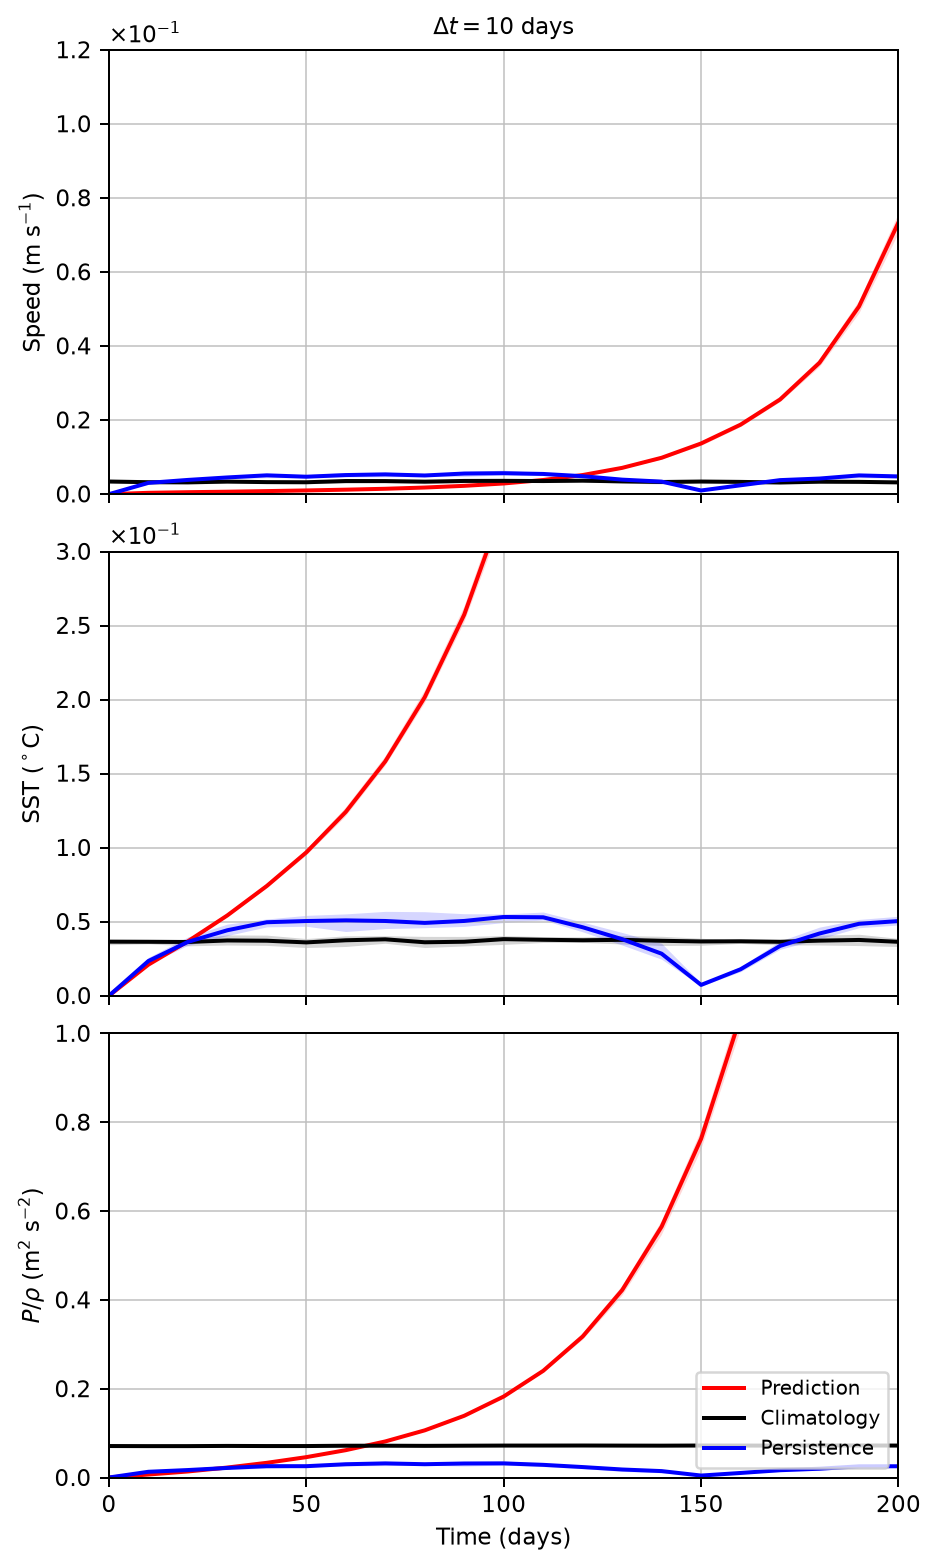
\includegraphics[height=0.75\textheight]{../outputs/af_fno/C/bire_figures_v1/model_c_bire_figure4_dt10_rmse_0_200_days.png}%
}{%
  \fcolorbox{amber}{lightamber}{\parbox[c][1.0in][c]{0.90\textwidth}{%
    \centering\textbf{Planned output; not generated}}}%
}\par
\small\color{graytext}Bire Figure-4 analogue for \(\Delta t=10\) days: mean RMSE
and 10th--90th percentiles over 15 fixed S2 starts.  Red is Model C, black is
leakage-free training climatology, and blue is persistence.  Axes are fixed exactly
as requested; red SST and pressure continue numerically beyond the visible limits
from days 100 and 160.
\end{center}

The paper-matched axes make the small black and blue baseline curves hard to inspect,
so the original output remains immutable and a separate descriptive addendum reads
only its hash-pinned NPZ archive.  It gives full-range and baseline-scale views for SST
and surface \(P/\rho\), plus a CSV containing every mean and 10th/90th percentile.
At day 10, mean SST RMSE is 0.0210 for Model C, 0.0235 for persistence, and
0.0365~\({}^{\circ}\mathrm{C}\) for climatology.  At day 20 these become
0.03681/0.03642/0.03635, so Model C first loses both baselines there.  Surface
\(P/\rho\) RMSE at day 10 is 0.00671/0.01287/0.07063
\(\mathrm{m^2\,s^{-2}}\); it first loses persistence at day 30
(0.02243 versus 0.02155) and climatology at day 70
(0.08117 versus 0.07156).

\widefigure
  {../outputs/af_fno/C/bire_baseline_zoom_v1/model_c_bire_figure4_dt10_sst_phihyd_full_and_zoom.png}
  {Baseline-visible companion to the immutable Figure-4 analogue.  Left panels retain
  the full finite Model-C range; right panels expose persistence and leakage-free
  training climatology.  Red is Model C, blue persistence, and black climatology.}

Contract SHA-256 \texttt{2a2324090b83...b2a4a} binds this addendum to the original
report/arrays.  The figure and CSV SHA-256 values are
\texttt{1f1ea2c6f76a...6643f}/\texttt{542e74c02b59...068ce}; manifest-content
SHA-256 is \texttt{01433936e406...99063}.  The package is under
\path{outputs/af_fno/C/bire_baseline_zoom_v1/}.  It evaluates no checkpoint and opens
no data.

The immutable report/arrays SHA-256 values are
\texttt{b704b921444d...e300ac5}/\texttt{a73ac9bf2cc9...20b1}.  Both PNGs,
the lightweight summary, and the hash manifest are under
\path{outputs/af_fno/C/bire_figures_v1/}; manifest-content SHA-256 is
\texttt{258be6fabe13...827f}.  Inference remains sealed.

The completed package is immutable, so additional sensitive-scale maps use the new
contract \path{config/model_c_bire_streamfunction_leads_v1.json}, SHA-256
\texttt{ccb965e58bdc\allowbreak...\allowbreak ae1934c}.  Before reading the new
day-50--90 fields, it fixes the same S2 start 6335 and checkpoint and exactly eight
separate figures at days 20, 30, \ldots, 90.  Each contains truth, prediction, and
truth-minus-prediction at \(1^\circ\).  Truth/prediction share one symmetric scale
across every lead.  Each error map has a labeled lead-specific symmetric scale and
printed RMSE/max error, so its structure is visible; cross-lead color comparisons
must use those numerical labels.  Day 10 remains in the original composite.  The
new output is descriptive only and cannot tune or open inference.  GPU job 291135
completed normally in 35 seconds, with all predictions finite.

\begin{center}
\begin{tabular}{@{}rrrr@{}}
\toprule
\textbf{Lead (days)} & \textbf{RMSE (Sv)} &
\textbf{Max error (Sv)} & \textbf{Relative RMSE} \\
\midrule
20 & 0.0934 & 0.7240 & 0.700\% \\
30 & 0.1580 & 1.1285 & 1.184\% \\
40 & 0.1765 & 1.0752 & 1.323\% \\
50 & 0.1737 & 0.9424 & 1.302\% \\
60 & 0.1814 & 0.7208 & 1.360\% \\
70 & 0.2148 & 0.7454 & 1.610\% \\
80 & 0.2583 & 0.9580 & 1.936\% \\
90 & 0.2951 & 1.1713 & 2.211\% \\
\bottomrule
\end{tabular}
\end{center}

\widefigure
  {../outputs/af_fno/C/bire_streamfunction_leads_v1/model_c_bire_figure3_streamfunction_1deg_day020.png}
  {Separate day-20 view.  Truth and prediction use the package-wide
  \(\pm45.545\)-Sv scale; the error panel uses its disclosed
  \(\pm0.724\)-Sv scale.}

\widefigure
  {../outputs/af_fno/C/bire_streamfunction_leads_v1/model_c_bire_figure3_streamfunction_1deg_day090.png}
  {Separate day-90 view.  The gyre remains visually close at 2.211\% relative
  streamfunction RMSE, while the sensitive error panel exposes the growing boundary
  and basin-scale structure on its disclosed \(\pm1.171\)-Sv scale.}

All eight figures are saved separately under
\path{outputs/af_fno/C/bire_streamfunction_leads_v1/}.  Report/arrays SHA-256 values
are \texttt{71c6e1dc1f9a...89c206}/\texttt{b4126494d9c0...3bcd48}, and
manifest-content SHA-256 is \texttt{3b74d759d551...450ac7}.  Days 20--40 reproduce
the first package to FP32 roundoff.  The barotropic circulation is therefore much
better preserved through day 90 than SST or surface pressure; Model C's failure is
field- and objective-specific rather than a uniform collapse of every predicted
dynamic.

Streamfunction is mandatory for circulation stability and wind-response physics.  SSH
remains a mandatory
RMSE/ACC/drift/map diagnostic with bootstrap uncertainty, but is not an independent
one-number veto: Bire neither learned nor scored it separately, and derived surface
pressure already includes \(g\eta\).  SSH can still reject a model through instability
or gross climate drift.

\section{Previously established ten-day comparison}

These values come from the earlier all-inference-pair evaluation and remain useful as a
cross-check.  Lower than one beats persistence.

\begin{center}
\begin{tabular}{@{}lrrr@{}}
\toprule
\textbf{Grouped variable} & \textbf{A0 / persistence} &
\textbf{A / persistence} & \textbf{B / persistence} \\
\midrule
U & 0.395 & 0.169 & 0.179 \\
V & 0.912 & 0.467 & 0.465 \\
Temperature & 4.771 & 2.052 & 1.814 \\
SSH & 13.612 & 2.277 & 2.107 \\
\bottomrule
\end{tabular}
\end{center}

\textbf{Interpretation.}  A is unambiguously better than A0 on this held ten-day
comparison, especially for velocity.  B preserves that short-lead gain and modestly
improves temperature and SSH, but both remain worse than persistence.  At 100 days,
B's model/persistence ratios are 0.449, 0.997, 8.009, and 9.925 for U, V, temperature,
and SSH.  Relative to A at the same lead, B reduces those four errors to 0.521, 0.409,
0.450, and 0.405.  Thus rollout training works, but the frozen B objective did not solve
the slow-field failure.

\section{A0: adapted Bire architecture}

\resultbox{red}{lightred}{\textbf{Gate status:} \Fail.  The pre-pressure v1 45-member,
10--360-day package is finished.  A0 remained finite, masked, and bounded
(maximum normalized wet-state magnitude 18.63) and reproduced the sign and magnitude of
the streamfunction--wind slope (model/truth slope 0.897).  It failed the ten-day
surface-field, 20-day ACC, and one-year spectral gates.  Day-360 model/truth spectral
energy ratios were 6.48 for surface speed, 96.16 for SST, 281.46 for SSH, and 21.49 for
streamfunction.}

The v1 failure already prevents A0 from passing; pressure-complete v2 will be generated
for fair field-by-field comparison, not to reconsider or retrain A0.

\pairedfigures
{../outputs/af_fno/A0/forward_complete_v1/forward_rmse_vs_lead.png}
{Physical RMSE against persistence and training climatology.}
{../outputs/af_fno/A0/forward_complete_v1/forward_acc_vs_lead.png}
{Pointwise-climatology anomaly correlation.}

\widefigure
{../outputs/af_fno/A0/forward_complete_v1/forward_spatial_rmse_maps.png}
{A0 spatial RMSE for surface speed, SST, SSH, and streamfunction.  Emulator and persistence share a scale within each field.}

\pairedfigures
{../outputs/af_fno/A0/forward_complete_v1/forward_spectra.png}
{Ensemble-mean resolved spectra.}
{../outputs/af_fno/A0/forward_complete_v1/forward_western_boundary_rmse.png}
{First four wet cells from the western wall.}

\pairedfigures
{../outputs/af_fno/A0/forward_complete_v1/forward_stability_by_regime.png}
{One-year physical stability by wind regime.}
{../outputs/af_fno/A0/forward_complete_v1/forward_wind_response.png}
{Low/control/high response at fixed lead times.}

\section{Model A: modern state-residual baseline}

\resultbox{red}{lightred}{\textbf{Gate status:} \Fail{} on available mandatory
evidence; complete one-year characterization not run.  A is frozen and reproducible,
but its ten-day temperature and SSH errors are 2.052 and 2.277 times persistence, so it
cannot pass the forward gate.  Its 100-day ratios rise to about 17.8 and 24.5.  The
queued complete evaluation was cancelled with zero runtime because it could describe,
but not reverse, this disqualifying result.  Missing panels below are retained as
explicit planned-output placeholders rather than fabricated results.}

\pairedfigures
{../outputs/af_fno/A/forward_complete_v2/forward_rmse_vs_lead.png}
{Physical RMSE against persistence and training climatology.}
{../outputs/af_fno/A/forward_complete_v2/forward_acc_vs_lead.png}
{Pointwise-climatology anomaly correlation.}

\widefigure
{../outputs/af_fno/A/forward_complete_v2/forward_spatial_rmse_maps.png}
{Model A spatial RMSE for surface speed, SST, SSH, and streamfunction.}

\pairedfigures
{../outputs/af_fno/A/forward_complete_v2/forward_spectra.png}
{Ensemble-mean resolved spectra.}
{../outputs/af_fno/A/forward_complete_v2/forward_vertical_drift.png}
{Day-360 mean and variance drift by depth.}

\pairedfigures
{../outputs/af_fno/A/forward_complete_v2/forward_stability_by_regime.png}
{One-year physical stability by wind regime.}
{../outputs/af_fno/A/forward_complete_v2/forward_forcing_switch_response.png}
{Provisional same-state forcing-switch response.}

\section{Model B: frozen rollout/spectral/boundary ablation}

\resultbox{red}{lightred}{\textbf{Gate status:} \Fail{} on available mandatory
evidence; retain as a controlled ablation.  B greatly reduces A's 100-day error but
still has ten-day temperature and SSH errors 1.814 and 2.107 times persistence.
Its frozen validation objective was also poorly balanced: state, rollout, spectral,
and boundary terms contributed approximately 41.6\%, 39.0\%, 1.0\%, and 18.3\% of the
total.  This is evidence to redesign C's objective, not permission to retune B.}

\pairedfigures
{../outputs/af_fno/B/final_v1/model_b_one_step_skill.png}
{Ten-day Model B skill by grouped variable.}
{../outputs/af_fno/B/final_v1/model_b_rollout_skill.png}
{Ten-to-100-day rollout against persistence.}

\pairedfigures
{../outputs/af_fno/B/final_v1/model_b_western_boundary_skill.png}
{Western-boundary skill reveals where the local and boundary losses help or fail.}
{../outputs/af_fno/B/final_v1/a0_model_a_model_b_rollout.png}
{Controlled A0/A/B rollout comparison.}

\section{Models C and D: revised forward/response separation}

\begin{tabularx}{\textwidth}{@{}p{0.11\textwidth}p{0.26\textwidth}Y@{}}
\toprule
\textbf{Model} & \textbf{Frozen role} & \textbf{Decision rule} \\
\midrule
C & Best forward emulator under the bounded search in the project plan & Select only on validation.  Every U/V/temperature/SSH ten-day ratio must beat persistence; then rank worst-group error and 30/90/180-day physics scores.  Run the complete one-year inference package only after freezing. \\
D & Accepted C design plus local perturbation--response loss & Preserve an accepted C successor's ten-day state error within 5\%, lower blind response error by at least 25\%, and improve projected-gradient angle without adjoint supervision. \\
\bottomrule
\end{tabularx}

\subsection{Model C stage C0: architecture and data audit}

\resultbox{blue}{lightblue}{\textbf{Status: training-only gate passed; bounded
validation v1 rejected.}  C0/C1a established the architecture candidates and loss-v1 scale.  C1b, C1c,
and width-64 capacity tests are preserved scientific rejections.  Objective audit
287581 justified a bounded optimization test without opening validation.  In job
287583, loss v2 was rejected and the loss-v1 fivefold learning-rate decay passed the
complete 96-record gate at epoch 315, including exact three-step reload.  The result is
narrow---only that evaluated epoch passed every group.  The subsequent frozen search
used validation but rejected its selected architecture at the final three-seed gate.
No validation entered the training diagnosis, and no inference, I1/I2, response, or
adjoint datum has been read.}

\begin{tabularx}{\textwidth}{@{}p{0.25\textwidth}Y@{}}
\toprule
\textbf{Criticism of B / starting C} & \textbf{Implemented C0/C correction} \\
\midrule
Fifteen U, 15 V, 15 temperature, and one SSH channel were aggregated in one relative norm. & Equal mean of U, V, temperature, and SSH group losses; every group is reported separately. \\
B's spectrum compares hard-masked full states, for which persistence is already strong and the land discontinuity leaks energy. & Compare ten-day increments, crop the exact $60\times60$ wet rectangle, remove the spatial mean, and apply a Hann taper before radial binning. \\
Slow-field increments are small relative to normalized state magnitude. & Scale each channel's increment error with its RMS computed from training pairs only. \\
The 16-mode choice had not been tested with NeuralOperator's exact real-FFT convention. & Audit \((12,12),(16,16),(16,24),(24,16),(24,24)\), interpreting the last declared count as \(m_x/2+1\) stored real-FFT columns. \\
Width 64 could improve capacity but multiplies cost. & Start at 630,262 parameters (width 32); test 2,443,542 parameters (width 64) only if fit/capacity evidence warrants it. \\
\bottomrule
\end{tabularx}

\begin{center}\small
\begin{tabular}{@{}lrrrr@{}}
\toprule
\textbf{Modes} & \textbf{U increment} & \textbf{V increment} &
\textbf{Temperature increment} & \textbf{SSH increment} \\
\midrule
\((16,16)\) & 8.8\% & 24.0\% & 67.8\% & 85.6\% \\
\((16,24)\) & 9.0\% & 25.6\% & 68.1\% & 86.8\% \\
\((24,16)\) & 12.5\% & 32.9\% & 70.2\% & 89.0\% \\
\((24,24)\) & 13.5\% & 38.3\% & 71.7\% & 90.9\% \\
\bottomrule
\end{tabular}
\end{center}

\begin{center}\small
\begin{tabular}{@{}lrrrr@{}}
\toprule
\textbf{C1a term} & \textbf{Raw loss} & \textbf{Gradient norm} &
\textbf{Frozen weight} & \textbf{Weighted grad./state} \\
\midrule
State & 0.03018 & 1.965 & 1 & 1.000 \\
Increment & 1.89450 & 830.5 & 0.001 & 0.423 \\
Rollout & 0.06463 & 6.484 & 0.15 & 0.495 \\
Spectrum & 38.4904 & 40,763 & \(10^{-5}\) & 0.207 \\
Boundary & 0.07825 & 7.411 & 0.065 & 0.245 \\
\bottomrule
\end{tabular}
\end{center}

\textbf{Interpretation.}  All \((16,16)\) full-state fractions exceed 99.6\%, so the
slow-field failure is not evidence that full states need a larger global truncation.
Velocity changes are predominantly higher frequency and must rely on the local branch;
24 meridional modes help more than 24 zonal modes.  The normalized ten-day increment
RMS varies by a factor of 147 across channels, confirming the need for training-only
per-channel scaling.  Increment-RMS autocorrelation leaves about 290 effective U,
392 V, 278 temperature, and 398 SSH samples across the three regimes; low-wind S1 is
the most correlated.  Version 1 is adequate for the first bounded search, but raw pair
counts substantially overstate independence.

The C1a automatic proposal clipped increment and spectral coefficients at 0.01.  It was
rejected because those values would still yield weighted gradient ratios about
4.23 and 207 relative to state.  Rounded \emph{unclipped} coefficients instead meet the
declared targets closely, as the table shows.  Thus \(10^{-5}\) spectral weight is not
tantamount to removing spectra: the raw spectral gradient is about 20,700 times the
state gradient.  The later training-only diagnosis below established that loss v1 can
memorize every group when late optimization is stabilized.  No validated or frozen C,
and no D result, exists yet.  Intermediate-wind, response-inference, and adjoint
archives remain sealed.  Any later data expansion will be versioned as v2; existing v1
data and conclusions will not be replaced.

\subsection{Model C stage C1b: rejected slow-field increment gate}

\begin{center}\small
\begin{tabular}{@{}lrrrrrr@{}}
\toprule
\textbf{LR} & \textbf{U/pers.} & \textbf{V/pers.} & \textbf{T/pers.} &
\textbf{SSH/pers.} & \textbf{State max} & \textbf{Rollout} \\
\midrule
0.0010 & 0.226 & 0.404 & 1.802 & 2.888 & 0.0271 & 0.0314 \\
0.0005 & 0.254 & 0.442 & 1.285 & 2.032 & 0.0304 & 0.0312 \\
\bottomrule
\end{tabular}
\end{center}

\textbf{Decision.}  Job 285192 completed in 58m30s and is scientifically rejected,
not a runtime failure.  Both attempts reduced total loss by about 97.7\%, spectral loss
by about 99.1\%, and passed state, rollout, and boundary thresholds.  Only temperature
and SSH ten-day increments remained worse than persistence.  Persistence NRMSE on this
exact subset is U/V/temperature/SSH 0.968/0.954/0.981/0.948; therefore the failure is
not an artifact of assuming an exact baseline of one.

The 0.0005 attempt reached its best total at epoch 160.  Stage C1c therefore changed
only duration to 320 epochs before any loss or width change.  The revised runner
recorded the exact subset persistence baseline, full learning curves, and a
bitwise-reload-tested diagnostic checkpoint even on rejection.

\subsection{C1c duration and width-64 capacity results}

\begin{center}\small
\begin{tabular}{@{}lrrrrrr@{}}
\toprule
\textbf{Run / selected epoch} & \textbf{U/pers.} & \textbf{V/pers.} &
\textbf{T/pers.} & \textbf{SSH/pers.} & \textbf{Balanced SSH} &
\textbf{Passing epochs} \\
\midrule
Width 32, C1c / 315 & 0.206 & 0.353 & 0.979 & 1.219 & 1.219 & 0 / 64 \\
Width 64 / 305 & 0.145 & 0.292 & 1.083 & 1.385 & 1.302 & 0 / 64 \\
\bottomrule
\end{tabular}
\end{center}

\textbf{Decision.}  Jobs 285265 and 285325 completed every scheduled epoch, exact
checkpoint reload, and all non-increment memorization criteria.  They are scientific
rejections rather than operational failures even though the older runner returned
exit 1 after safely writing each rejected report.  C1c temperature first beat
persistence at epochs 310 and 315, but SSH never did; width 64 made the best balanced
SSH ratio worse.  Increasing duration or capacity again is therefore unsupported.

\subsection{Late-checkpoint objective audit}

\begin{center}\small
\begin{tabular}{@{}lrr@{}}
\toprule
\textbf{Training-only audit quantity} & \textbf{Width 32} & \textbf{Width 64} \\
\midrule
Weighted increment loss / state loss & 0.0569 & 0.0724 \\
Weighted increment gradient / state gradient & 0.4215 & 0.4064 \\
Effective SSH increment gradient / state gradient & 0.4137 & 0.3975 \\
Effective temperature increment gradient / state gradient & 0.0807 & 0.0841 \\
SSH increment--state gradient cosine & 0.9656 & 0.9271 \\
Total-gradient reconstruction relative error & \(9.0\times10^{-8}\) &
\(1.1\times10^{-7}\) \\
\bottomrule
\end{tabular}
\end{center}

GPU array 287581 independently rechecked all 64 evaluated epochs in each history,
verified the exact 96-record training subset and report/checkpoint provenance, and
differentiated each raw and weighted component over the full-record mean.  The
increment term is small by objective value but is not absent from optimization: its
weighted gradient is about 41\% of the state gradient and is dominated by an aligned
SSH component.  Together with the volatile late SSH ratios, this supports testing a
bounded late-optimization stabilization before changing capacity or data.  Separately,
operational scaling job 287556 measured 436/272/253 seconds at 4/8/16 CPU cores.
Sixteen cores is therefore the fallback if the GPU queue would materially delay useful
work; this benchmark does not motivate a backend-replication study.

\subsection{Bounded objective/optimizer decision}

\begin{center}\small
\begin{tabular}{@{}p{0.31\textwidth}rrrrr@{}}
\toprule
\textbf{Isolated variant / selected epoch} & \textbf{U/pers.} &
\textbf{V/pers.} & \textbf{T/pers.} & \textbf{SSH/pers.} &
\textbf{Decision} \\
\midrule
Loss v1; LR \(5{\times}10^{-4}\rightarrow10^{-4}\) after 240 / 315 &
0.211 & 0.360 & 0.794 & 0.990 & Pass \\
Loss v2; increment weight 0.0025 / 315 &
0.213 & 0.357 & 1.058 & 1.770 & Reject \\
\bottomrule
\end{tabular}
\end{center}

\resultbox{green}{lightteal}{\textbf{Training-only decision: accept the loss-v1
learning-rate decay for bounded validation.}  Job 287583 task 0 reduced total and
spectral loss by 98.24\% and 99.82\%; maximum state-group error was 0.0248,
rollout/boundary were 0.0231/0.0301, and reloaded three-step output was bitwise exact.
Every increment group beat persistence at epoch 315.  Only that epoch passed all
groups, and epoch 320's SSH ratio returned slightly above one, so this is a narrow
memorization pass rather than evidence of validation skill.}

The accepted checkpoint/report SHA-256 values are
\texttt{b383c69ce337...0bb6d1} and \texttt{95b6dc85159b...025aa}.
Task 1's higher-increment loss v2 is preserved as a versioned rejected branch; even its
best balanced epoch had SSH at 1.328 times persistence.  The contrast favored optimizer
stabilization, not a loss revision, and justified the now-complete bounded validation
search reported below.  Inference, I1/I2, response, and adjoint data remain sealed.

\resultbox{blue}{lightblue}{\textbf{Validation protocol frozen before metrics.}
\path{config/model_c_validation_search_v1.json}, SHA-256
\texttt{9e1d44299ae6...c4c6f6}, fixes ten base candidates and four from-scratch
successive-halving rounds.  Chronology/step budgets are
25\%/1,920, 50\%/3,840, 75\%/5,760, and 100\%/7,680.  Each round uses the accepted
75\%-point fivefold learning-rate decay.  All 780 ten-day validation pairs and 48 fixed
long-rollout starts determine the predeclared lexicographic groupwise and
30/90/180-day physics ranking.  The final design is not frozen unless all three fixed
seeds independently beat persistence for every ten-day group and reload exactly.}

\subsection{Bounded Model C validation result}

All 20 candidate jobs across the four stages completed with scheduler exit code zero,
finite reports, immutable checkpoints, matching source/data/normalizer contracts, and
bitwise-exact three-step reload.  Only training and validation split codes 1 and 2
were read.  Thus the outcome below is scientific, not operational.

\begin{center}\small
\begin{tabular}{@{}lrrlp{0.28\textwidth}@{}}
\toprule
\textbf{Stage / job} & \textbf{Chronology} & \textbf{Steps} &
\textbf{Leading worst ratio} & \textbf{Declared survivors} \\
\midrule
1 / 287604 & 25\% & 1,920 & 2.030, \texttt{m16\_24\_w64} &
\texttt{m16\_24\_w64}, \texttt{m24\_16\_w64}, \texttt{m24\_24\_w64},
\texttt{m12\_12\_w64}, \texttt{m12\_12\_w32} \\
2 / 288466 & 50\% & 3,840 & 1.470, \texttt{m16\_24\_w64} &
\texttt{m16\_24\_w64}, \texttt{m24\_16\_w64}, \texttt{m12\_12\_w64} \\
3 / 289379 & 75\% & 5,760 & 1.153, \texttt{m16\_24\_w64} &
\texttt{m16\_24\_w64}, \texttt{m24\_16\_w64} \\
4 / 289915 & 100\% & 7,680 & 1.00014, \texttt{m24\_16\_w64} &
\texttt{m24\_16\_w64} for the independent seed gate \\
\bottomrule
\end{tabular}
\end{center}

The stage-manifest SHA-256 values are, in order,
\texttt{40b54530d7d9...12d2f05}, \texttt{a2d639f8940c...d5e382},
\texttt{9bbd4fc4ce3c...f30e17}, and \texttt{453c05ec408f...2fea2}.
At full resources, the \((24,16)\), width-64 candidate had
U/V/temperature/SSH ratios 0.1473/0.3547/0.6597/1.00014 and physics score 22.84;
the \((16,24)\), width-64 candidate had 0.1577/0.3723/0.6353/1.02477 and score 28.22.
The selected design fit the full training chronology in every group
(worst ratio 0.915).  Both finalists were below the training-underfit threshold
(0.915/0.941), and their western-boundary/full-domain ratios were 0.667/0.639,
well below the 1.25 wall-leakage trigger.  The search therefore correctly opened
neither the six-layer nor 20\%-padding branch.

\begin{center}\small
\begin{tabular}{@{}lrrrrrrc@{}}
\toprule
\textbf{Seed} & \textbf{Step} & \textbf{U} & \textbf{V} &
\textbf{Temperature} & \textbf{SSH} & \textbf{Physics score} &
\textbf{Reload} \\
\midrule
20260723 & 7,440 & 0.1473 & 0.3547 & 0.6597 & 1.00014 & 22.84 & Exact \\
20260724 & 7,680 & 0.1472 & 0.3531 & 0.6442 & 1.00383 & 24.86 & Exact \\
20260725 & 7,680 & 0.1512 & 0.3612 & 0.7034 & 1.03818 & 21.49 & Exact \\
\bottomrule
\end{tabular}
\end{center}

\resultbox{red}{lightred}{\textbf{Scientific decision: reject validation-search v1.}
The frozen rule requires every seed and every ten-day group to be strictly below
persistence.  All three seeds fail only SSH, so the near equality for two seeds cannot
be rounded into a pass.  The immutable decision, SHA-256
\texttt{e19d502442fc...72155}, records
\texttt{configuration\_frozen=false} and
\texttt{inference\_authorized=false}; its internal freeze-contract SHA-256 is
\texttt{a44622cee685...73628}.}

The longer validation rollouts reinforce rather than soften this decision.  Across the
three seeds, the full-domain mean group ratio is 0.704--0.765 at 30 days, but rises to
3.21--3.45 at 90 days and 53.54--61.90 at 180 days; the aggregate physics score is
21.49--24.86.  Hence the candidate is close only at the primary ten-day SSH boundary
and is not a stable long-horizon forward emulator.

The \texttt{m24\_16\_w64} worst-group curve nevertheless improves monotonically with
chronology: 2.168, 1.483, 1.192, and 1.00014 at 25/50/75/100\%.  Full-chronology
aggregate training fit passes and the final SSH spread is nonzero.  The subsequently
frozen per-regime/autocorrelation audit passed its expansion gate, but showed that
aggregate pooling hides S1 training underfit.  Therefore the authorized v2 expansion is
a controlled data-scale experiment, not evidence that architecture and objective are
already adequate.  The current architecture must be retrained unchanged on v2 before
the bounded successor variants are interpreted.  Inference and all later archives
remain sealed.

\section{S0 Bire-style Figures 3--8: completed long-horizon test}

\resultbox{green}{lightteal}{\textbf{Short-to-medium result: best Model C so far.}
Job 304736 evaluated the frozen seed-20260724, step-13,440 checkpoint at
\(\tau_0=0.1~\mathrm{N\,m^{-2}}\) and \(\Delta t=10\) days for 15
inference initializations.  At day 200, model/persistence/climatology RMSE is
\(0.00270/0.00457/0.00351~\mathrm{m\,s^{-1}}\) for surface speed,
\(0.0151/0.0198/0.0625~\mathrm{m^2\,s^{-2}}\) for surface \(P/\rho\),
and \(0.0241/0.0488/0.0391~{}^\circ\mathrm{C}\) for SST.}

The selected/prior-residual day-200 mean ACC values are 0.784/0.107 for
surface U, 0.887/0.033 for surface V, 0.972/0.003 for surface \(P/\rho\),
and 0.833/\(-0.036\) for SST.  Figure~6 is therefore an
architecture-direction comparison, not a literal pretrained/fine-tuned pair:
the selected anomaly/direct-state model was trained from scratch.

\begin{center}\small
\begin{tabular}{@{}lrrrr@{}}
\toprule
\textbf{Field} & \textbf{Day-200 model} & \textbf{Persistence} &
\textbf{Climatology} & \textbf{Day-2,000 model} \\
\midrule
Surface speed (\(\mathrm{m\,s^{-1}}\)) & 0.00270 & 0.00457 & 0.00351 & 0.426 \\
Surface \(P/\rho\) (\(\mathrm{m^2\,s^{-2}}\)) & 0.0151 & 0.0198 & 0.0625 & 2.593 \\
SST (\({}^\circ\mathrm{C}\)) & 0.0241 & 0.0488 & 0.0391 & 5.339 \\
\bottomrule
\end{tabular}
\end{center}

\resultbox{red}{lightred}{\textbf{Long-term result: finite is not stable.}
All 15 states remain numerically finite, but by day 2,000 the model is
81.9/67.7/87.1 times persistence and 108.9/30.4/128.1 times climatology for
speed/\(P/\rho\)/SST.  The day-2,000 model 10th--90th percentile intervals
are 0.372--0.463, 2.371--2.825, and 3.838--6.484 in their respective units,
so the failure is ensemble-wide.  The fixed member's streamfunction RMSE
grows from 0.294~Sv at day 60 (correlation 0.9996) to 96.2~Sv at day 2,000
(correlation \(-0.183\)).  Model C therefore fails the Bire-style
long-term-statistical stability requirement even though it is excellent over
the deterministic forecast window.}

\widefigure
  {../outputs/af_fno/C/anomaly_direct_bire_s0_inference_v1/model_c_bire_figure3_streamfunction_1deg_s0_dt10.png}
  {Figure-3 analogue for the fixed inference member.  Truth, selected Model C,
  and error retain an accurate basin-scale streamfunction through day 40.}

\widefigure
  {../outputs/af_fno/C/anomaly_direct_bire_s0_inference_v1/model_c_bire_figure4_dt10_rmse_0_200_days_s0.png}
  {Figure-4 analogue.  Lines are 15-member means and bands are memberwise
  10th--90th percentiles; red is Model C, blue persistence, and black the
  training-only pointwise S0 climatology.  Model C beats both baselines at
  day 200 for all three fields.}

\widefigure
  {../outputs/af_fno/C/anomaly_direct_bire_s0_inference_v1/model_c_bire_figure5_dt10_single_member_rmse_s0.png}
  {Figure-5 analogue for start index 6913.  At day 200, streamfunction and
  SST RMSE are 0.657~Sv and \(0.0232~{}^\circ\mathrm{C}\).}

\widefigure
  {../outputs/af_fno/C/anomaly_direct_bire_s0_inference_v1/model_c_bire_figure6_dt10_acc_0_200_days_s0.png}
  {Figure-6 analogue.  Red is the selected anomaly/direct-state Model C and
  black the prior residual rollout-conditioned Model C; this is a
  representation-direction comparison, not literal fine-tuning.}

\widefigure
  {../outputs/af_fno/C/anomaly_direct_bire_s0_inference_v1/model_c_bire_figure7_dt10_streamfunction_day060_day2000_s0.png}
  {Figure-7 analogue.  A single shared scale preserves honest amplitude
  comparison: the day-2,000 model range dominates the page because its
  streamfunction has become unstable, while day-60 agreement remains close.}

\widefigure
  {../outputs/af_fno/C/anomaly_direct_bire_s0_inference_v1/model_c_bire_figure8_dt10_rmse_0_2000_days_s0.png}
  {Figure-8 analogue.  The same 15-member ensemble that is skillful through
  day 200 develops a coherent runaway at longer lead, whereas both MITgcm
  baselines remain bounded.}

The complete package is
\path{outputs/af_fno/C/anomaly_direct_bire_s0_inference_v1/}.  Arrays/report
SHA-256 is \texttt{30abd95810d3...3c7}/
\texttt{32ac2e051726...bd18}; report-content SHA-256 is
\texttt{9711016c7fca...e022}; manifest-content SHA-256 is
\texttt{593dd43de772...57d1}.  These results support continuing with the
anomaly/direct-state representation for short deterministic forecasts, but
they do not authorize a long-term-stability claim or replace the separate
learned-physics wind-response assessment.

\resultbox{green}{lightteal}{\textbf{Boundary mechanism result: common,
ensemble-coherent runaway; checkpoint age is not the cure.}  V100 job
304740 completed normally in 1m46s with zero retraining.  All seven
checkpoints remain finite but cross mean maximum normalized amplitude 20 by
day 880.  The earlier 3,840/7,680/11,520 checkpoints cross on days
410/580/780, whereas selected step 13,440 crosses latest at day 880.
Shorter training therefore worsens rather than removes this instability.
The diagnostic is descriptive and does not reselect the checkpoint.}

The boundary result is strong spatially.  The four-cell wet-boundary union
contains 896 of 3,600 wet cells, or 24.9\%, but at selected step 13,440 it
holds 72.8\%, 85.2\%, and 72.7\% of ensemble-mean day-2,000
\(Q_x\), \(Q_y\), and streamfunction squared error.  Boundary/interior
RMSE is \(147.4/51.1~\mathrm{m^2\,s^{-1}}\) for \(Q_x\),
\(100.6/23.8~\mathrm{m^2\,s^{-1}}\) for \(Q_y\), and
192.7/63.3~Sv for streamfunction.  This is not one exceptional member:
member-to-ensemble-mean day-2,000 spatial cosine is
0.783/0.649/0.902, and hotspot sign agreement is
93.2/88.5/97.1\% for \(Q_x/Q_y/\psi\).

The temporal mechanism is subtler.  Selected-model boundary/interior
day-200-relative \(2\times/5\times/10\times\) crossing days are
360/620/860 versus 340/570/840 for \(Q_x\),
360/600/790 versus 340/550/820 for \(Q_y\), and
660/920/1,260 versus 320/590/920 for streamfunction.  Boundary error is
larger and disproportionate, but it does not consistently start growing
before the interior.  The supported classification is a systematic,
boundary-amplified global transport mode.  The experiment does not support a
simple boundary-to-interior propagation cascade, nor does it isolate padding
as the cause.

\widefigure
  {../outputs/af_fno/C/anomaly_direct_bire_s0_boundary_checkpoint_v1/model_c_s0_boundary_transport_rmse_checkpoints.png}
  {Depth-integrated zonal-transport RMSE by checkpoint and region.  Every
  checkpoint grows, while the selected step 13,440 is among the least
  unstable and is not improved by reverting to an earlier checkpoint.}

\widefigure
  {../outputs/af_fno/C/anomaly_direct_bire_s0_boundary_checkpoint_v1/model_c_s0_boundary_fraction_checkpoints.png}
  {Fraction of total squared error inside the four-cell wet-boundary union.
  The dotted 0.249 line is the boundary cell fraction; transport and
  streamfunction errors are spatially overrepresented there.}

\widefigure
  {../outputs/af_fno/C/anomaly_direct_bire_s0_boundary_checkpoint_v1/model_c_s0_checkpoint_stability_timing.png}
  {Checkpoint-age diagnosis.  All checkpoints cross every plotted amplitude
  threshold, with selected step 13,440 crossing 20/100 on days 880/1,610.}

\widefigure
  {../outputs/af_fno/C/anomaly_direct_bire_s0_boundary_checkpoint_v1/model_c_s0_selected_boundary_spatial_consistency.png}
  {Selected-model day-2,000 spatial consistency across 15 members.  The
  western and northeastern streamfunction/transport hotspots recur with high
  pattern and sign agreement.}

\widefigure
  {../outputs/af_fno/C/anomaly_direct_bire_s0_boundary_checkpoint_v1/model_c_s0_selected_boundary_growth.png}
  {Selected-model boundary versus interior error growth.  Boundary RMSE is
  persistently larger, but its relative growth thresholds do not
  consistently precede the interior.}

All ten manifest-listed artifacts verify against their SHA-256 and byte
counts.  Report/summary/arrays SHA-256 is
\texttt{bc62501a18f7...2fc67}/\texttt{c6c069e52ee5...fef50e}/
\texttt{d37d570337a3...b9942ae}; report-content SHA-256 is
\texttt{0a370f256a39...155345} and manifest-content SHA-256 is
\texttt{134afea7b726...ce562}.  The complete package is
\path{outputs/af_fno/C/anomaly_direct_bire_s0_boundary_checkpoint_v1/}.

\resultbox{green}{lightteal}{\textbf{Instrument correction: the day-200
boundedness check was too short.}  The post-hoc, zero-rollout contract
\path{config/model_c_s0_stability_instrument_v1.json}, SHA-256
\texttt{ab6d597843b1...fc5be7}, reads only immutable job-304736 arrays.
Over days 300--600, fitted RMSE gain per ten-day call is
1.0332 [1.0297, 1.0369] for speed, 1.0397 [1.0391, 1.0401] for surface
\(P/\rho\), and 1.0456 [1.0424, 1.0485] for SST, where intervals are
10,000-replicate member bootstraps.  All remain supercritical over days
1,700--2,000 at 1.0321/1.0240/1.0227.}

Maximum absolute normalized state is only 3.49 at initialization and 3.75
at day 200, then reaches 5.57 at day 300 and 322.39 at day 2,000.  Its
days-300--600 gain is 1.0252 per call, an approximately 401-day e-folding.
Thus the failure is present as sustained multiplicative growth before the
former reporting horizon, even though its amplitude is visually modest at
day 200.

\widefigure
  {../outputs/af_fno/C/anomaly_direct_s0_stability_instrument_v1/model_c_s0_rmse_log_growth.png}
  {The job-304736 Figure-8 curves on logarithmic axes.  After the
  approximately 90-day decorrelation horizon, both baselines remain bounded
  while Model C continues nearly linearly in log error.}

\widefigure
  {../outputs/af_fno/C/anomaly_direct_s0_stability_instrument_v1/model_c_s0_windowed_rmse_gain.png}
  {Windowed multiplicative RMSE gain with 95\% member-bootstrap intervals.
  Every field and every fitted window remains above one.}

\widefigure
  {../outputs/af_fno/C/anomaly_direct_s0_stability_instrument_v1/model_c_s0_normalized_amplitude_log_growth.png}
  {Normalized-amplitude growth.  The former day-200 check precedes the
  sustained threshold crossings and cannot establish long-term boundedness.}

The fitted RMSE gain is descriptive; it is not the Jacobian spectral radius
and is not a sufficient stand-alone gate for a chaotic forecast.  The
corrected future instrument keeps the 10--90-day deterministic skill gate
separate, then requires post-decorrelation saturation, a truth-relative
normalized-amplitude envelope, time-averaged field means/variances and
low/mid/high spectral energy, and streamfunction extrema/mean circulation
through at least 200 calls.  Local operator work will report singular gain
and finite-time tangent growth unless eigenvalue analysis is actually
performed.

LayerNorm is therefore a causal control, not the presumed solution.  It does
not mathematically bound the full autoregressive map, and the completed
LayerNorm-only arm already misses the protected day-360 gate at
mid/bottom ratios 9.74/4.92 with 18.6\% worst primary degradation.  A
zero-retraining 2,000-day comparison remains useful to test whether it lowers
growth, but it cannot supersede the selected model without passing both
short-skill and statistical-stability criteria.

All six manifest-listed artifacts verify.  Report/content/manifest-content
SHA-256 is \texttt{5212f3aee081...72040}/
\texttt{945495f0e096...6cfbe}/\texttt{f03aeb9487ab...869a}; the package is
\path{outputs/af_fno/C/anomaly_direct_s0_stability_instrument_v1/}.

\resultbox{amber}{lightamber}{\textbf{Original diagnostic failed
operationally; evaluation-only recovery frozen.}  Contract
\path{config/model_c_s0_stability_tangent_comparison_v1.json}, SHA-256
\texttt{5d32d472509a...bca4}, permitted zero retraining and no checkpoint
selection.  Job 304750 exited 1 after 1m42s because explosive float32
physical reductions overflowed and the log-fit rejected the non-finite
series.  No transactional result package was published.}

The long-rollout half records speed, surface \(P/\rho\), SST, and
streamfunction means/variances; truth-relative normalized-amplitude
envelopes; RMSE growth over days 300--600, 700--1,000, and 1,700--2,000;
and radial spectra at days 200/500/1,000/1,500/2,000.  Truth is the immutable
job-304735 S0 \MITgcm{} continuation, while climatology remains the
training-only S0 pointwise temporal mean.

The local-operator half uses three fixed training-only S0 states.  It
estimates dominant one-step singular gain and ten-call tangent geometric
gain for full, \(k=1\)--3, \(k=4\)--9, and \(k=10\)--30 perturbations.
Only the selected and LayerNorm direct-state maps enter this tangent
comparison because they share pointwise-normalized state coordinates; the
prior residual map's different coordinates would make a raw norm ranking
misleading.  No result is labeled a spectral radius.  Three focused tests,
lint, shell validation, source/artifact hashes, complete-truth coverage, and
CPU finite/land-zero one-step reloads of all three models pass.  Four plots,
NPZ, CSV, report, summary, README, and manifest are reserved under
\path{outputs/af_fno/C/anomaly_direct_s0_stability_tangent_comparison_v1/}.

Recovery contract
\path{config/model_c_s0_stability_tangent_recovery_v2.json}, SHA-256
\texttt{8bc5c0937d0e...e1ac}, preserves the failed job and every model,
checkpoint, initial condition, lead, truth field, spectrum band, and tangent
state.  It changes only physical reductions to float64, records first
non-finite model-state lead per member, and censors a fit at its first
incomplete all-member sample.  Four focused tests verify large-amplitude
overflow safety, agreement with the original diagnostics at physical
amplitudes, and exact censoring behavior.  Preflight and all three one-step
reloads pass.  Recovered numerical results remain pending under
\path{outputs/af_fno/C/anomaly_direct_s0_stability_tangent_recovery_v2/};
no model may be trained, selected, or promoted.

\resultbox{green}{lightteal}{\textbf{Recovery result: LayerNorm strongly
reduces but does not cure the runaway.}  Job 304751 completed normally in
2m12s.  Every state remains finite through day 2,000, proving that finiteness
is not a stability gate.  The prior residual map caused the original
float32 diagnostic overflow and is catastrophically unstable, not
contracting.}

At day 2,000, mean speed/\(P/\rho\)/SST RMSE is
0.4260/2.5933/5.3391 for selected Model C,
0.0217/0.5525/0.4218 for LayerNorm, and
\(3.32\times10^{25}/6.76\times10^{26}/1.41\times10^{27}\) for the prior
residual map.  Relative to climatology, the three triplets are
108.89/30.44/128.10, 5.54/6.48/10.12, and
\(8.48\times10^{27}/7.93\times10^{27}/3.39\times10^{28}\).
LayerNorm therefore removes 94.9/78.7/92.1\% of selected error but still
fails Bire-style statistical stability.  Its normalized-amplitude ratio to
same-time truth is 4.01, versus 63.57 selected and
\(1.94\times10^{26}\) prior.

Every LayerNorm growth window remains supercritical.  Days-300--600
speed/\(P/\rho\)/SST gain per call is
1.02045/1.02177/1.02702; days-1,700--2,000 gain remains
1.00330/1.00541/1.00646.  It crosses and then stays worse than climatology
on days 270/530/300.  Its day-2,000 circulation is also wrong:
streamfunction ensemble-mean extrema are \(-78.5/17.6\)~Sv versus
\(-30.0/34.1\)~Sv truth, and spatial standard deviation is 16.77 versus
10.67~Sv.

The spectral result identifies the controlled part of the mechanism.
LayerNorm day-2,000 high-\(k\) power ratio for
speed/\(P/\rho\)/SST/streamfunction is 25.5/38.9/77.0/31.5, much smaller
than selected Model C's 3,335/9,240/13,237/10,207 but still unacceptable.
At day 200, the corresponding LayerNorm ratios are only
1.04/1.32/1.05/1.60, so a small tail grows persistently after the former
reporting horizon.  The prior residual map already has day-200 high-\(k\)
ratios 104/11,193/3,226/232 and subsequently dominates the log plots.

The local tangent result is not a simple contraction ranking.  Averaged over
three training-only S0 states, selected versus LayerNorm full-field
one-step singular gain is 4.04 versus 3.66 and ten-call gain is 1.020
versus 1.117.  In the high-\(k\) band LayerNorm improves
3.65/0.992 to 2.36/0.964, but in the mid-\(k\) band it worsens
3.34/1.085 to 4.07/1.130.  Thus LayerNorm's long-run benefit is consistent
with selective high-\(k\) suppression and changed nonlinear off-manifold
dynamics, not uniform local contractivity.  It simultaneously degrades
day-30 speed/\(P/\rho\)/SST RMSE by 9.1/36.8/8.6\% relative to selected,
so it cannot be promoted.

\widefigure
  {../outputs/af_fno/C/anomaly_direct_s0_stability_tangent_recovery_v2/model_c_s0_stability_models_log_rmse.png}
  {Float64-recovered S0 RMSE through day 2,000.  The prior residual map
  grows almost linearly on the log scale to \(10^{25}\)--\(10^{27}\);
  LayerNorm substantially flattens the direct-state runaway but remains
  above climatology and keeps growing.}

\widefigure
  {../outputs/af_fno/C/anomaly_direct_s0_stability_tangent_recovery_v2/model_c_s0_stability_normalized_envelope.png}
  {Truth-relative method-native normalized amplitude.  Day-2,000 ratios are
  63.57 selected, 4.01 LayerNorm, and \(1.94\times10^{26}\) prior.}

\widefigure
  {../outputs/af_fno/C/anomaly_direct_s0_stability_tangent_recovery_v2/model_c_s0_stability_day2000_spectra.png}
  {Day-2,000 power relative to truth.  LayerNorm selectively suppresses the
  selected model's extreme mid/high-\(k\) excess but does not restore a
  statistically plausible spectrum.}

\widefigure
  {../outputs/af_fno/C/anomaly_direct_s0_stability_tangent_recovery_v2/model_c_s0_tangent_gain_comparison.png}
  {Shared-coordinate local tangent audit.  LayerNorm damps high-\(k\)
  response but has larger mid-\(k\) and full-field ten-call gain; no
  uniform-contraction claim is supported.}

\widefigure
  {../outputs/af_fno/C/anomaly_direct_s0_stability_tangent_recovery_v2/model_c_s0_first_nonfinite_lead.png}
  {All 15 members of every map remain finite through day 2,000.  The
  catastrophic prior residual curve demonstrates why finiteness cannot
  substitute for amplitude and statistical-climate gates.}

All ten manifest-listed artifacts and both scratch/project copies verify.
Contract/arrays/report/summary SHA-256 is
\texttt{8bc5c0937d0e...e1ac}/\texttt{95e0a42bc437...01175}/
\texttt{684815b7882b...7b84}/\texttt{bdd7c1a06c0d...cc25};
report-content/manifest-content SHA-256 is
\texttt{05e92283b2a0...00dd}/\texttt{30a5288053ef...c4e5}.  The complete
package is
\path{outputs/af_fno/C/anomaly_direct_s0_stability_tangent_recovery_v2/}.
Retain selected Model C only for the accepted short forecast role.  The next
bounded control should test high-\(k\) suppression or a gated normalization
path while explicitly protecting short skill; a blanket Jacobian-norm
penalty is not authorized by these data.

\resultbox{amber}{lightamber}{\textbf{Fixed high-\(k\) damping rejected.}
Job 304753 completed normally in 1m07s under contract
\path{config/model_c_s0_highk_damping_control_v1.json}, SHA-256
\texttt{cf2f1c179d36...9554}.  Every nonzero strength fails the prospective
training gate, so inference remains sealed and no filter or checkpoint is
selected.}

The candidate strengths are \(\alpha=0,0.02,0.05,0.10,0.20\), where
zero is exact selected Model C and nonzero values blend each predicted
normalized anomaly with a channelwise \(3\times3\) binomial smoothing.
Selection uses only ten fixed S0 starts with complete day-1,000 windows in
split 1.  A nonzero strength must keep all day-10/30/90 primary RMSE within
5\% of source, reduce day-1,000 worst RMSE/climatology and normalized
amplitude to 80\% of source, and halve worst high-\(k\) power.  The smallest
passing value alone opens the frozen 15-member S0 day-2,000
characterization.

The weakest intervention, \(\alpha=0.02\), passes all three long-horizon
requirements.  At day 1,000, worst RMSE/climatology, normalized amplitude,
and worst high-\(k\) power are respectively
0.7768/0.7742/0.4448 of the unfiltered source.  It fails the 5\% short guard:
worst short RMSE is 1.0658 times source at day-90 SST, while day-90 speed is
1.0612 times source.  For \(\alpha=0.05/0.10/0.20\), worst short ratios
increase to 1.5000/2.2640/3.3406.  Thus smoothing produces a monotonic
short-skill cost even as it removes the long-horizon tail.

\widefigure
  {../outputs/af_fno/C/anomaly_direct_s0_highk_damping_control_v1/model_c_s0_highk_training_selection.png}
  {Prospective training-only filter selection.  Weak damping jointly lowers
  day-1,000 RMSE, normalized amplitude, and high-\(k\) power, but no nonzero
  strength stays within the frozen 5\% short-skill guard.}

This intervention supports high-\(k\) content as a causal contributor to the
off-manifold runaway, but rejects fixed isotropic smoothing as sufficient.
The useful short-range SST/speed scales and unstable tail are not separable
with one constant post-step \(\alpha\).  The conditional inference phase was
correctly not run; do not weaken the guard or tune another fixed strength.
The next bounded correction should integrate a state- or scale-aware gate
into training while using the unfiltered short forecast as an explicit
reference.

All nine manifest-listed artifacts verify, and the scratch/project arrays
and report are byte-identical.  Contract/arrays/report/summary SHA-256 is
\texttt{cf2f1c179d36...9554}/\texttt{88eac7163328...9d}/
\texttt{8ca08f114763...a66}/\texttt{3c100081bd10...806};
report-content/manifest-content SHA-256 is
\texttt{856612ebb748...e11}/\texttt{248c1b2e9a8a...057}.  The complete
package is
\path{outputs/af_fno/C/anomaly_direct_s0_highk_damping_control_v1/}.

\resultbox{amber}{lightamber}{\textbf{Scale-selective filter rejected.}
Job 304754 completed normally in 1m06s under contract
\path{config/model_c_s0_reflected_spectral_gate_control_v1.json}, SHA-256
\texttt{69b0100aae27...b8e7}.  No nonzero strength passes, so fixed
inference remains sealed and no filter or checkpoint is selected.}

The wet \(60\times60\) rectangle is extended evenly in both directions,
avoiding a periodic seam.  The frozen radial transfer is exactly one for
\(k\leq8\), a cosine transition over \(8<k<10\), and \(1-\alpha\) for
\(k\geq10\), with \(\alpha=0,0.25,0.50,0.75,1.00\).  This isolates scale
selectivity from the previous all-scale binomial smoothing: it asks whether
the 5\% short guard and the three day-1,000 reduction gates can overlap when
low modes are untouched.  Only the smallest passing nonzero strength may
open the unchanged fixed 15-member S0 inference characterization.

At \(\alpha=0.25\), day-1,000 normalized amplitude, worst high-\(k\) power,
and worst RMSE/climatology are 0.4365/0.0638/0.6178 of the source.  The
intervention therefore removes 93.6\% of source high-band power.  It does
not recover a plausible state: amplitude remains 3.65 times truth and worst
RMSE remains 4.41 times climatology.  It also destroys short skill.  SST
day-10/30/90 RMSE is 5.30/6.49/5.94 times source, and the corresponding
worst ratios for \(\alpha=0.50/0.75/1.00\) rise to
10.45/15.63/20.82.

\widefigure
  {../outputs/af_fno/C/anomaly_direct_s0_reflected_spectral_gate_control_v1/model_c_s0_reflected_spectral_training_selection.png}
  {Training-only reflected spectral-gate result.  High-band power and
  long-horizon amplitude fall sharply, but short forecast error rises by
  factors of 6--21 and absolute day-1,000 statistics remain implausible.}

The high-\(k\) excess is therefore a coupled symptom and amplifier, not the
sole instability source or a safely removable component.  Fixed
postprocessing is closed.  The next forward-model study should directly test
the unresolved channel bottleneck: Bire assigns width 128 to ten outputs,
whereas selected Model C assigns the same width to 46.  Establish a reduced
ten-output Bire-facing model and require deterministic 10--90-day skill plus
bounded statistical day-2,000 behavior before resuming the complete adjoint
campaign.  Do not require post-decorrelation trajectory RMSE to beat
persistence indefinitely.

All nine manifest-listed artifacts verify, and scratch/project arrays and
reports are byte-identical.  Contract/arrays/report/summary SHA-256 is
\texttt{69b0100aae27...b8e7}/\texttt{74827af0d9e6...e164}/
\texttt{2b739a495fc8...ec53}/\texttt{0e2f11d7fba3...4a36};
report-content/manifest-content SHA-256 is
\texttt{84e7b3521a54...85c3}/\texttt{018af80f1942...154d}.  The complete
package is
\path{outputs/af_fno/C/anomaly_direct_s0_reflected_spectral_gate_control_v1/}.

\resultbox{blue}{lightblue}{\textbf{Arm R frozen; numerical results pending.}
Contract \path{config/model_c_reduced_channel_control_v1.json}, SHA-256
\texttt{a1b8ce50d1b...5a6c5}, isolates the 46-versus-10-output hypothesis.
It changes the selected Model C dynamical task to ten Bire-facing channels
while preserving the direct pointwise-anomaly map, width-128 four-block
trunk, modes, padding, optimizer, checkpoints, and three-step objective
form.}

The exact ordered state is surface/mid \(U\), surface/mid \(V\),
surface/mid temperature, surface/mid/bottom \texttt{PHIHYD}, and barotropic
streamfunction.  The latter four diagnostics are derived only when building
truth targets and are predicted directly thereafter.  Thus the rollout is a
genuine reduced closure: it cannot consult or reconstruct any omitted
46-channel state after initialization.  The semantic loss groups are
U/V/temperature/\texttt{PHIHYD}/streamfunction with the original term
weights; this unavoidable adaptation is explicit in the contract.

The derived cache is 2.2~GB with shape
\(3\times7200\times10\times62\times62\).  Logical-state SHA-256 is
\texttt{b24728abf50f...c5aa}, metadata/quality SHA-256 is
\texttt{3ec92a0b30d6...253}/\texttt{b8842dea6f50...a50}, and four
split-spanning snapshots reproduce fresh 46-to-10 reconstruction bitwise.
Pooled split-1 pointwise mean/raw-scale/final-scale/floor SHA-256 is
\texttt{3e2c26c3f6db...9687}/\texttt{b9bb679751ab...d3f}/
\texttt{6a2d4c7403c1...117f}/\texttt{e2cb5043bec1...e0f2}.

Training selection uses seed 20260724, seven checkpoints through step 15,360,
and the unchanged 540 split-1 starts through day 90.  After selection, the
runner automatically computes the same six S0 Figure~3--8 analogues as
\path{anomaly_direct_bire_s0_inference_v1}: identical 15 starts, day-2,000
truth, persistence, S0 training climatology, wet-cell reductions, ensemble
summaries, and filenames.  Figure~6 directly compares the retained
46-channel source in black with Arm R in red.  A failed training gate still
receives the fixed descriptive long evaluation requested here, but cannot be
promoted.

Six focused tests, lint, shell validation, both source-locked preflights, and
a \(62\times62\) three-call forward/loss smoke test pass; all outputs are
finite with exact zero land leakage.  Parameter count is 14,823,642.
Training artifacts will be stored under
\path{/bigscratch/mjalabert314/bire_james25_repro/af_fno/models/C/anomaly_direct_reduced_channel_control_v1/};
the complete six-figure package will be published under
\path{outputs/af_fno/C/anomaly_direct_reduced_channel_bire_s0_inference_v1/}.
No adjoint authorization follows from completion alone.

\section{Arm R falsifies the channel-count hypothesis}

\resultbox{red}{lightred}{\textbf{Channel count is not the cause.}  Arm R reduces the
autoregressive state from 46 to the ten Bire-facing outputs, raising the latent-per-output
ratio from 2.78 to 12.8, and holds seed, normalization, trunk, modes, padding, optimizer,
checkpoints, and the three-step objective form fixed.  It is roughly 20\% \emph{better}
short-term and passes both of its own gates, yet the per-call error growth rate is
unchanged.  A 4.6-fold increase in conditioning per output rescaled the runaway without
removing it.}

\begin{center}\small
\begin{tabular}{@{}lrrrrr@{}}
\toprule
\textbf{Field} & \textbf{d30} & \textbf{d90} & \textbf{d200} &
\textbf{d2,000 (46ch)} & \textbf{d2,000 (Arm R)} \\
\midrule
Surface speed (\(\mathrm{m\,s^{-1}}\)) & 0.774 & 0.803 & 0.963 & 0.426 & 0.242 \\
SST (\({}^\circ\mathrm{C}\)) & 0.708 & 0.811 & 0.935 & 5.339 & 2.149 \\
Surface \(P/\rho\) (\(\mathrm{m^2\,s^{-2}}\)) & 0.938 & 0.861 & 0.751 & 2.593 & 11.500 \\
\bottomrule
\end{tabular}
\end{center}

The first three columns are Arm R divided by the retained 46-channel model; the last two
are absolute day-2,000 ensemble-mean RMSE.  Arm R day-2,000 error is still
61.8/51.6/135.0 times climatology for speed/SST/\(P/\rho\).  Per-ten-day-call RMSE gains
over days 300--600 are 1.0325/1.0455/1.0401 for the 46-channel model and
1.0247/1.0396/1.0627 for Arm R; over days 1,700--2,000 they are 1.0320/1.0229/1.0241 and
1.0376/1.0255/1.0204.  Surface pressure is 4.4 times \emph{worse} at day 2,000 under the
reduced state, so removing the deep temperature levels also removes information the
hydrostatic closure needs.  This eliminates channel count and latent conditioning as
explanations, alongside depth/padding, output-head interference, and both fixed
high-\(k\) postprocessing controls.

\subsection{The duplicated positional encoding}

Position currently enters the forward map twice.  The 51 input channels already contain
\texttt{longitude\_normalized} and \texttt{latitude\_normalized} from
\path{src/bire_repro/af_data.py}, and the \MITgcm{}-facing FNO is constructed with
\texttt{positional\_embedding="grid"}, so \texttt{GridEmbeddingND} appends two further
coordinate channels immediately before lifting.  Both encodings are computed on the same
unpadded \(62\times62\) grid, so the lifting block receives 53 channels carrying 51
distinct fields.  Bire et al.\ encode position exactly once (Section 3.3.1, two
sine/cosine channels before lifting).  Removing the appended grid embedding drops 512
lifting weights, so this is a redundancy and conditioning correction, not a capacity
change; the parallel \(3\times3\) local branch still sees the two static position
channels.

\subsection{Two gate clauses were mis-specified}

Four consecutive controls failed the same two clauses, and both are defective rather than
demanding.  The deep-pressure clause requires the median mode-wise model-over-truth energy
ratio at levels 7 and 14 to stay at or below four at every ten-day lead through day 360.
Its denominator is the truth high-wavenumber energy, about \(2\times10^{-6}\) of the
field, so the clause thresholds numerical noise on a \emph{derived} quantity.  In both
prior controls the day-360 mid integrated energy ratio was 1.00--1.03, inside the retained
\([0.8,1.25]\) bound, while only the mode-wise ratio failed at 9.2--12.5.  The
short-lead clause caps degradation at 1.1 times the incumbent, but every stabilizing
change costs short-lead sharpness: the LayerNorm checkpoint is 1.05/1.17/1.82 times the
incumbent at day 90 while remaining 0.278/0.248/0.368 of persistence and
0.413/0.363/0.189 of climatology.  It is therefore vetoed for being worse than the
incumbent while comfortably satisfying the actual scientific requirement.

\subsection{Frozen single-position LayerNorm arm}

Contract \path{config/model_c_anomaly_direct_single_position_layernorm_v1.json} returns to
the full 46-channel pointwise-anomaly direct-state Model C and changes exactly two things:
the appended grid embedding is disabled, and the Bire pointwise channel LayerNorm is
applied after spectral and Channel-MLP mixing.  Seed 20260724, normalization, modes,
width, depth, padding, optimizer, the seven checkpoint steps, and the 540 split-1
selection rollouts are unchanged.  The source-relative veto moves from 1.1 to 2.0 and the
deep-pressure mode-wise ratio becomes reported-not-a-veto with the integrated energy bound
retained, both recorded explicitly under \texttt{gate\_corrections}; the principled fix,
restricting the mode-wise statistic to modes carrying the truth's cumulative 99\% energy,
requires a code change and is deferred rather than applied.  On a passing training gate the
same six Figure~3--8 filenames, the same 15 S0 starts, and the same reductions are
republished under
\path{outputs/af_fno/C/anomaly_direct_single_position_layernorm_v1/}, with the log-scale
RMSE, per-call gain intervals, and day-2,000 spatial standard-deviation ratio added.  On
failure the declared successor is a tangent-penalty arm targeting the dominant one-step
singular gain in the diagnosed \(k=4\)--9 band; no threshold tuning is authorized.

\section{Single-position LayerNorm arm: first passing gate and first
near-neutral map}

\subsection{Training-only result}

Job 305203 trained the arm in 1h13m and selected optimizer step 14,880 with
\texttt{arm\_training\_gate\_passed} (14,863,446 parameters).

\begin{center}\small
\begin{tabular}{@{}rrrrrrc@{}}
\toprule
\textbf{Step} & \textbf{Worst primary} & \textbf{Rel.\ source} &
\textbf{Mode-wise} & \textbf{Mid int.} & \textbf{Bot.\ int.} & \textbf{Pass} \\
\midrule
11,520 & 1.1911 & 3.495 & 45.21 & 0.995 & 1.058 & No \\
13,440 & 0.7343 & 2.155 & 14.52 & 0.868 & 0.972 & No \\
14,400 & 0.7482 & 2.195 & 12.42 & 0.920 & 1.017 & No \\
\textbf{14,880} & \textbf{0.4716} & \textbf{1.384} & \textbf{9.50} &
\textbf{1.035} & \textbf{1.043} & \textbf{Yes} \\
15,360 & 0.6859 & 2.013 & 9.93 & 1.043 & 1.016 & No \\
\bottomrule
\end{tabular}
\end{center}

\resultbox{red}{lightred}{\textbf{The gate correction, not the architecture change,
produced the first pass.}  Re-scoring the already-trained parent LayerNorm arm --- the
one that \emph{keeps} the duplicated positional encoding --- against the corrected gate
shows it passing at both step 14,400 (0.4042/1.186/9.74) and step 14,880
(0.3253/1.067/10.17).  At step 14,880 it satisfies the primary clause, the
integrated-energy clause, and even the \emph{original} 1.1 source-relative cap; it
failed the original gate \emph{solely} on the deep-pressure mode-wise clause.  That
clause alone had been blocking a checkpoint that was already trained.}

On training-only 10--90-day error the single-position arm is the weakest of the four
controls: 0.4716 against 0.3253 for the parent LayerNorm arm, 0.3596 for group heads,
and 0.3855 for three layers without padding.  Removing the duplicated encoding costs
short-lead accuracy.

\subsection{Held S0 evaluation}

Job 310508 published the same six Figure 3--8 plots, the same 15 starts, the same
day-2,000 truth, the same baselines, and the same filenames as
\path{anomaly_direct_bire_s0_inference_v1}, under
\path{outputs/af_fno/C/single_position_layernorm_bire_s0_inference_v1/}.

\begin{center}\small
\begin{tabular}{@{}lrrrr@{}}
\toprule
\textbf{Field} & \textbf{Day 200} & \textbf{Day 2,000} &
\textbf{Day 2,000 (46ch)} & \textbf{Gain 1,700--2,000} \\
\midrule
Surface speed & 0.00280 & \textbf{0.0316} & 0.426 & \textbf{1.0082} (was 1.0320) \\
SST & 0.0228 & \textbf{0.4155} & 5.339 & \textbf{1.0019} (was 1.0229) \\
Surface \(P/\rho\) & 0.0305 & \textbf{0.4822} & 2.593 & \textbf{1.0011} (was 1.0241) \\
\bottomrule
\end{tabular}
\end{center}

\resultbox{green}{lightteal}{\textbf{Long-horizon behaviour is a different regime.}
Day-2,000 error falls 13.5/12.8/5.4-fold and the asymptotic per-call gain collapses from
1.023--1.032 to 1.0011--1.0082, with SST and surface pressure within 0.2\% of a
non-expanding map.  This is also below the plain LayerNorm arm's 1.003--1.007.  All 15
states remain finite.  Short-term skill is retained: at day 90 the arm is
0.29/0.22/0.53 of persistence and 0.43/0.32/0.27 of climatology for
speed/SST/\(P/\rho\), beating both baselines on every primary field.  Day-200 ACC is
0.844/0.833/0.926/0.862 for U/V/\(P/\rho\)/SST.}

Two caveats belong with that result.  First, surface pressure regresses at short lead:
day-200 RMSE rises from 0.0151 to 0.0305 and now \emph{loses} to persistence there
(1.54 times) while still beating climatology (0.49 times); speed and SST are unaffected.
Second, and more consequential for the protocol, the training gate ranked these arms in
close to the opposite order to their long-horizon behaviour.  The arm with the worst
10--90-day error has by far the best autoregressive gain.  This is direct evidence that
the training-only gate is still not measuring the quantity the project needs, and it
argues for promoting the per-call gain from a reported diagnostic to a selection
criterion.

\subsection{Provenance correction}

The frozen figure runner hard-codes \texttt{step-13440} in its published README text, so
the first attempt (job 308944) published a package whose README misdescribed the model.
The package was withdrawn and regenerated by job 310508 with an arm-specific README; the
numerical artifacts reproduce bitwise.  A regression test now asserts that the published
README names step 14,880 and that the frozen runner's own text is unchanged.

\section{Bire-aligned full-state FNO: architecture package, learning rate, and
protocol faithfulness}

Three new training arms test whether a substantially more faithful Bire architecture
and training protocol transfers to the 46-channel closed state.  All three keep the
\MITgcm{} trajectories, the \(62\times62\) grid, the \((24,16)\) modes, the 46-channel
state, the ten-day map, the pointwise anomaly normalization, and the held S0 evaluation
fixed, and replace the remaining project-specific choices with the Bire choice: three
FNO blocks instead of four, six pointwise channel LayerNorms instead of eight, the exact
deterministic \texttt{oceanfourcast.PosEmbed} sine/cosine position fields appended
immediately before lifting instead of linear longitude/latitude data channels, no
external \(3\times3\) raw-input branch, and the wet-cell \(\mathrm{MSE}+w\,\mathrm{MAE}\)
objective instead of the five-term Model C loss.  Channel bookkeeping is
\(46+3=49\) external inputs, \(49+2=51\) lifting inputs, and 46 outputs; the two linear
coordinate fields are removed so that absolute position enters exactly once.  The wet
mask and distance-to-wall field are retained because they encode basin geometry rather
than generic absolute coordinates.  Every arm trains 3,840 one-step pretraining updates
followed by 3,840 two-step autoregressive fine-tuning updates at batch size 8 with
Adam\((\beta_1,\beta_2)=(0.9,0.95)\), zero weight decay, and no gradient clipping, and
retains both stage checkpoints.  All three have 11,154,478 parameters against the
incumbent's 14,863,446.

\subsection{Learning rate \texorpdfstring{$10^{-2}$}{1e-2}: collapse to climatology}

The contract
\begin{quote}
\path{config/model_c_bire_aligned_full_state_v1.json}\\
SHA-256 \texttt{62aed544703f...a71363}
\end{quote}
adopts the paper's Table~2 learning rate of 0.01.
Job 311335 completed normally in 17m46s without a non-finite loss or gradient, so the
declared fail-fast clause never fired.  It nevertheless produced no forecast skill.

\begin{center}\small
\begin{tabular}{@{}lrrrrc@{}}
\toprule
\textbf{Stage} & \textbf{Speed} & \textbf{SST} & \textbf{\(P/\rho\)} &
\textbf{Mode-wise} & \textbf{Pass} \\
\midrule
Pretrained (3,840) & 2.3785 & 3.1837 & 19.5907 & 1.033 & No \\
Fine-tuned (7,680) & 2.3754 & 3.1821 & 19.5644 & 0.954 & No \\
\bottomrule
\end{tabular}
\end{center}

\resultbox{red}{lightred}{\textbf{The model collapsed to the climatological field, and
the project's stability instruments scored that as a success.}  Training MSE settled at
0.978 in normalized units, where predicting exactly zero anomaly gives 1.0 by
construction.  Day-360 mode-wise ratio 0.95 and integrated energy 0.96--1.00 are the best
values any arm has produced, and the day-2,000 normalized amplitude is 4.87 against the
incumbent's 76.7 --- because emitting the climatological field is trivially stable.
Day-200 ACC is \(+0.06/+0.06/+0.32/+0.09\) for U/V/\(P/\rho\)/SST against the incumbent's
\(+0.844/+0.833/+0.926/+0.862\).  Reading only the long-horizon diagnostics would have
recorded this as the stability fix.}

A controlled 600-step diagnostic on the identical code path, data, and seed separated the
two candidate explanations: at \(10^{-2}\) the one-step normalized MSE stays at
1.03--0.94, while at \(5\times10^{-4}\) it reaches 0.034 against a persistence value of
0.0185.  The trained checkpoints emit \texttt{pred\_rms} 0.041 and 0.012, and their
one-step MSE matches the zero-prediction MSE to four decimals.  The collapse is therefore
attributable to the learning rate, not to the architecture package.  The paper's Table~2
explains why it does not transfer: Bire's 0.01 belongs to a \(248\times248\) grid with
\((64,64)\) retained modes and \(C_{\mathrm{in}},C_{\mathrm{out}}=11,10\), roughly ten
times our spectral operator and a quarter of our channels.

\subsection{Learning rate \texorpdfstring{$5\times10^{-4}$}{5e-4}: a real model with a
bounded but displaced attractor}

The contract
\begin{quote}
\path{config/model_c_bire_aligned_full_state_lr5e4_v1.json}\\
SHA-256 \texttt{b00f741562fc...2633b3}
\end{quote}
is a one-factor control: the loader reloads the parent
contract and asserts that architecture, loss, stages, gate, seed, batch size, betas,
weight decay, clipping, and step budget are equal field by field, so the learning rate is
the only quantity that moves.  Job 311831 completed in 31m34s.

\begin{center}\small
\begin{tabular}{@{}lrrrrc@{}}
\toprule
\textbf{Stage} & \textbf{Speed} & \textbf{SST} & \textbf{\(P/\rho\)} &
\textbf{Worst} & \textbf{Below persistence} \\
\midrule
Pretrained (3,840) & 0.7437 & 0.8308 & 3.4657 & 3.4657 & No \\
\textbf{Fine-tuned (7,680)} & \textbf{0.4312} & \textbf{0.4210} & \textbf{0.9518} &
\textbf{0.9518} & \textbf{Yes} \\
\bottomrule
\end{tabular}
\end{center}

Two-step fine-tuning does substantial work here: the worst primary ratio falls from 3.466
to 0.952 and surface pressure alone improves 3.466 to 0.952.  This reproduces Bire's own
claim that multistep fine-tuning improves autoregressive prediction, and it is invisible
in the \(10^{-2}\) arm because there was nothing to improve.  The gate still fails the
source-relative clause at 2.793 against the 2.0 limit.

\resultbox{amber}{lightamber}{\textbf{On held S0 the arm is bounded but settles on a
displaced attractor, not on climatology.}  Day-2,000 RMSE saturates at 3.28/4.72/3.93
times climatology and stays flat from roughly day 500 onward; the 1,700--2,000-day
per-call gain is 1.0011/1.0002/1.0000 and the normalized amplitude reaches only 7.91.
All 15 members converge to the same state --- day-2,000 SST RMSE has member standard
deviation 0.009 on a mean of 0.197 --- so this is a fixed point rather than chaos.  The
day-2,000 barotropic streamfunction still correlates 0.971 with truth at a spatial
standard-deviation ratio of 1.105, so the circulation is nearly right and the error is
thermodynamic.  Short-lead skill is far below the incumbent: day-200 ACC is
\(+0.402/+0.396/+0.539/+0.226\) and day-200 RMSE is 2.28/3.66/4.54 times climatology.}

\subsection{Protocol faithfulness bundle: neutral to negative}

Three unintended divergences from the public \texttt{oceanfourcast} implementation
survived the earlier arms and were corrected as one bundle on the \(5\times10^{-4}\)
base under \path{config/model_c_bire_aligned_faithful_v1.json}, SHA-256
\texttt{7c3e012dae74...a9729a}: the MAE weight becomes 0.05 rather than 0.01, because
\texttt{train.py} computes \(\mathrm{criterion}+0.05\,\mathrm{criterion2}\) in all four of
its training and validation functions; the step decay becomes
\texttt{CosineAnnealingLR} with \(T_{\max}=3\) and \(\eta_{\min}=10^{-5}\); and the
checkpoint retained per stage becomes the one minimising validation loss over a seeded
random 10\% holdout of split-1 training records, with the running best reset when
fine-tuning begins.  Channel-MLP dropout stays at zero: the repository defaults it to
0.5, but the paper's hyperparameter table does not specify it, and 0.5 is a strong
regulariser rather than a faithfulness correction.  Job 314709 completed in 20m43s.

\begin{center}\small
\begin{tabular}{@{}lrrrrr@{}}
\toprule
\textbf{Arm (fine-tuned)} & \textbf{Speed} & \textbf{SST} & \textbf{\(P/\rho\)} &
\textbf{ACC\(_{200}\) U} & \textbf{Day-2,000 \(\times\)clim} \\
\midrule
\(5\times10^{-4}\) base & 0.4312 & 0.4210 & 0.9518 & \(+0.402\) & 3.28/4.72/3.93 \\
Faithfulness bundle & 0.4712 & 0.4485 & \textbf{0.8926} & \(+0.261\) & 3.93/4.63/4.50 \\
\bottomrule
\end{tabular}
\end{center}

\resultbox{red}{lightred}{\textbf{The training gate and the held S0 evaluation disagreed
in direction for the third time.}  On the gate the bundle improves the worst primary
ratio 0.9518 to 0.8926 by fixing surface pressure.  On held S0 it \emph{loses} skill on
the field the base arm was strongest at: day-200 surface-U ACC falls from \(+0.402\) to
\(+0.261\), SST is flat, and only pressure improves to \(+0.588\).  The day-2,000 tail
does not move.  The bundle redistributes skill from the velocity fields to the
thermodynamic fields rather than adding any.}

Two attribution limits belong with that result.  Validation-based selection was a no-op:
validation loss fell monotonically within each stage
(\(0.0198\!\rightarrow\!0.0098\) and \(0.0172\!\rightarrow\!0.0144\)), so it selected
epochs 2 and 4, which are exactly the fixed steps 3,840 and 7,680 the earlier arms used.
The mechanism is in place and correct but changed nothing here, so it cannot explain any
part of the difference.  The MAE weight and the cosine schedule therefore moved together
and this arm cannot separate them.  Adopting validation selection also costs 10\% of the
training records (13,446 against 14,940), which is inherent to the mechanism rather than
a free choice.

\subsubsection*{Erratum: stale objective prose in the faithfulness contract}

The faithfulness contract's authoritative \texttt{loss.mae\_weight} is 0.05 and the
runner reads that field, so job 314709 is numerically correct.  Its two \emph{stage}
objective strings, however, still read \(\mathrm{MSE}+0.01\,\mathrm{MAE}\).  The cause is
the single-change assertion itself: it required \texttt{stages} to equal the parent arm's
block verbatim, which forced the parent's stale prose through unchanged.  The completed
contract is left byte-identical because its SHA-256 is recorded in the run's report, and
editing it now would break that provenance chain for a purely descriptive defect.  The
mechanism is fixed instead: the loss-recovery loader below rejects any stage objective
string that contradicts the authoritative numeric fields, and a regression test exercises
that rejection.

\subsection{Loss-recovery control: the objective, not the architecture, cost the
skill}

The three arms above leave one suspect.  Bire's \(\mathrm{MSE}+w\,\mathrm{MAE}\)
averages over all 46 normalized channels, which gives the physical groups effective
multiplicities \(U:V:\Theta:\eta = 15:15:15:1\): the free surface receives \(1/46\) of
the channel-averaged loss while each of \(U,V,\Theta\) receives \(15/46\).  That is not
equivalent to Bire's problem, because they predicted several \texttt{PHIHYD} levels and
the streamfunction directly whereas this model predicts only \((U,V,\Theta,\eta)\) and
reconstructs pressure and circulation afterwards.  The objective therefore leaves the
free surface, barotropic circulation, hydrostatic pressure, and the slow basin-scale
modes weakly constrained --- exactly the quantities that decide which attractor a long
rollout approaches.

The contract
\begin{quote}
\path{config/model_c_bire_aligned_loss_recovery_v1.json}\\
SHA-256 \texttt{4932821d0b46...f8c570}
\end{quote}
is the architecture-fixed control.  It keeps the three-block map, \((24,16)\) modes,
width 128, six pointwise LayerNorms, the Bire position fields, the absent external
\(3\times3\) branch, 10\% padding, Adam at \(5\times10^{-4}\) with betas
\((0.9,0.95)\), zero weight decay, no clipping, batch size 8, and the 7,680-step budget,
and changes only the objective and the rollout exposure back to the incumbent
group-balanced Model C loss v1,
\[
\mathcal L_{\mathrm{state}}=\frac{1}{4}\left(\mathcal L_U+\mathcal L_V+
\mathcal L_\Theta+\mathcal L_\eta\right),
\]
with its increment, rollout, spectral, and western-boundary terms over a three-step
unrolled rollout.  Job 314770 completed in 39m00s.

\begin{center}\small
\begin{tabular}{@{}lrrrrr@{}}
\toprule
\textbf{Arm (same map, same optimizer, same budget)} & \textbf{Speed} & \textbf{SST} &
\textbf{\(P/\rho\)} & \textbf{Worst} & \textbf{Rel.\ source} \\
\midrule
Bire \(\mathrm{MSE}+0.01\,\mathrm{MAE}\) & 0.4312 & 0.4210 & 0.9518 & 0.9518 & 2.793 \\
\textbf{Incumbent loss v1} & \textbf{0.4455} & \textbf{0.3888} & \textbf{0.4532} &
\textbf{0.4532} & \textbf{2.008} \\
\bottomrule
\end{tabular}
\end{center}

\resultbox{green}{lightteal}{\textbf{The field starved by the channel weighting is the
field that recovers.}  Surface pressure more than halves on the training gate, 0.9518 to
0.4532, while speed and SST barely move --- precisely what the \(15{:}15{:}15{:}1\)
multiplicity argument predicts.  On held S0 the effect is larger still: the 10--90-day
RMSE ratio to persistence falls from 2.072 to \textbf{0.398} for surface pressure, from
0.734 to 0.395 for SST, and from 0.560 to 0.436 for speed, so this arm beats persistence
on all three primary fields.  Its day-200 pressure ACC rises from \(+0.54\) to
\(+0.85\), against the incumbent's \(+0.93\), and its short-lead pressure ratio 0.398 is
now \emph{better} than the incumbent's 0.415.  The day-2,000 tail stays bounded and flat:
per-call gain over 1,700--2,000 days is 1.0001/1.0008/1.0000 and the normalized amplitude
is 7.1.}

This is the first branch of the predeclared decision table --- short-term skill recovers
while the day-2,000 error remains flat --- so the Bire-aligned architecture is useful and
the Bire objective was the problem.  Two qualifications belong with it.  The training
gate still records \texttt{no\_arm\_checkpoint\_passed}, failing the source-relative
clause at 2.008 against the 2.0 limit, a margin of 0.008.  And the day-2,000 pressure
level moves the wrong way: 3.93 to 6.47 times climatology, while speed is unchanged at
3.30 and SST improves slightly to 4.28.  The tail is flat but its pressure attractor sits
further from climatology, so the wrong-invariant-distribution problem is not solved by
reweighting alone.  The training window was still falling monotonically at step 7,680
(0.330, 0.180, 0.145, 0.090), so this arm is not converged.

\subsection{Strictly chronological split: prospective skill is much weaker, the
displaced attractor is not}

Every result above was obtained under the stored split, whose training block
(0--2519 and 3690--6209) surrounds the validation block in time and so supports an
interpolation claim rather than a prospective one.  The contract
\begin{quote}
\path{config/model_c_bire_aligned_loss_recovery_chronological_v1.json}\\
SHA-256 \texttt{276830e38ac3...8a7ae6}
\end{quote}
retrains the loss-recovery model, unchanged in every architectural and optimizer
respect and from scratch on the same seed, under train 0--5039, then validation 5130--5759, then test 5850--7199,
with 90-day buffers at both boundaries.  Every train-derived statistic ---
pointwise mean, pointwise scale, channel floors, per-regime climatology, and the
pointwise increment scale --- is recomputed from 0--5039 alone; reusing the
incumbent normalizer would import 5040--6209, which is validation or test here.
Wind normalization is unchanged because \texttt{static\_features} has no time
axis.  Checkpoint selection moves to 90 held 360-day rollouts inside the
validation block under the declared rule.

This is not a pure reordering.  Both training sets hold 5,040 days but only 3,870
overlap: 5040--6209 is exchanged for 2520--3689, so 23.2\% of the training
snapshots change.  The arm tests the chronological protocol \emph{and}
sensitivity to the training period.

Job 317123 completed in 47m19s.  Validation selected step 7,680, which dominated
every field and both lead windows, so the short-skill guard never bound.

\begin{center}\small
\begin{tabular}{@{}lrrr@{}}
\toprule
\textbf{Evaluation block} & \textbf{Speed} & \textbf{SST} & \textbf{\(P/\rho\)} \\
\midrule
Validation 5130--5759, 10--90-day AUC / persistence & 0.480 & 0.472 & 0.560 \\
Held S0 test 6660--7199, 10--90-day RMSE / persistence & 1.175 & 1.161 & 6.202 \\
\midrule
Stored-split arm on the same S0 block & 0.436 & 0.395 & 0.398 \\
\bottomrule
\end{tabular}
\end{center}

\resultbox{red}{lightred}{\textbf{The same checkpoint looks good on validation and
loses to persistence on test.}  Day-200 ACC falls from \(+0.63/+0.64/+0.93/+0.56\)
on validation to \(+0.26/+0.09/+0.66/+0.11\) on the held S0 block, and the
10--90-day error rises from 0.47--0.56 of persistence to 1.16--6.20.  Against the
stored-split arm evaluated on the identical 15 starts, short-lead skill is two to
sixteen times worse.  This is the second predeclared outcome: part of the earlier
result depended on temporally interleaved training coverage, and true prospective
generalization is substantially weaker than the stored protocol suggested.}

The mechanism is decorrelation distance, not distribution drift.  Sampled S0
wet-cell means move by only \(-0.0045\,^\circ\mathrm{C}\) in SST and
\(+4.5\times10^{-4}\) in \(\eta\) between the training and test blocks, so the
climate is effectively stationary.  What differs is how far each evaluation block
sits beyond the end of training: validation starts are 91--352 days after index
5039, whereas the S0 test starts are 1,623--2,160 days after it.  This project's
own slow-field audit measured S0 SSH spatial-anomaly \(e\)-folding at 248 days,
with S1/S2 still above \(e^{-1}\) at 720 days.  The 630-day validation block,
placed immediately after training behind a 90-day buffer, therefore lies
\emph{inside} the slow-field correlation window and over-estimates prospective
skill; the 90-day buffer was sized for a ten-day pair horizon, not for slow-field
decorrelation.  The stored-split arm scored well on the same S0 starts for the
same reason: it trained through 6209, only 453--990 days before them.

\resultbox{green}{lightteal}{\textbf{The displaced attractor is intrinsic to the
map and objective, not to the split or the normalization.}  Day-2,000 error is
3.33/3.81/5.62 times climatology against the stored-split arm's 3.30/4.28/6.47,
with per-call gain 1.0009/1.0002/1.0000 and amplitude 7.2 against 7.1.  Changing
the training period, recomputing every train-derived statistic, and moving
checkpoint selection to held data leave the long-horizon behaviour essentially
unchanged.  This is the fourth predeclared outcome and it removes the split and
the normalizer as explanations, which is what justifies a targeted
attractor-supervision experiment.}

Two qualifications.  The training window was still falling monotonically at step
7,680 (0.321, 0.176, 0.144, 0.090), so this arm is no more converged than its
parent, and the contract explicitly defers the duration continuation.  And the
comparison confounds three things at once --- the chronological protocol, the
23.2\% change of training period, and the extra 1,170 days of distance between
the end of training and the test block --- so it bounds prospective skill rather
than isolating a single cause.

\subsection{Independent-wind trajectory-v3 simulations}

Every arm above trained on trajectory-v2, in which S1 and S2 were branched from
the S0 year-100 state and given a five-year adjustment under their own wind.
That construction makes the three regimes share a common history, so a
wind-regime comparison partly measures how far each branch has travelled from a
single state rather than how the circulation differs between winds.
Trajectory-v3 removes the shared history: each regime is a 125-year integration
started from the same \MITgcm{} double-gyre tutorial initial condition under its
own wind --- 100 years of equilibration followed by 25 years of daily production
output --- with no branching between regimes.  S0 is the original control
lineage, whose spin-up was already independent by construction; S1 and S2 were
newly integrated for this dataset under \path{mitgcm_independent_v1}.

\begin{center}\small
\begin{tabular}{@{}lrrl@{}}
\toprule
\textbf{Regime} & \(\tau_0\) \textbf{(N m\(^{-2}\))} &
\textbf{Wind scale} & \textbf{Construction} \\
\midrule
S0 & 0.100 & \(1.00\times\) & Independent 100-y spin-up, then 25 y daily \\
S1 & 0.075 & \(0.75\times\) & Independent 100-y spin-up, then 25 y daily \\
S2 & 0.125 & \(1.25\times\) & Independent 100-y spin-up, then 25 y daily \\
\bottomrule
\end{tabular}
\end{center}

The regimes differ in zonal wind amplitude and in nothing else: bathymetry, the
SST relaxation, the executable, the 1{,}200\,s timestep, and the 360-day year are
identical, and the wind fields were verified to be exactly \(1.00/0.75/1.25\)
times the tutorial field.  The new runs were carried out on CPU with pickup chaining, every join
hash-verified.  All three regimes span iterations \(2{,}592{,}000\)--\(3{,}239{,}928\),
model years \(100.000\)--\(124.997\), with gaps of exactly 72 steps (one model
day) throughout, so each is one continuous 125-year integration rather than a
concatenation of independent restarts.  The realised wind maxima are
\(0.099863\), \(0.074897\) and \(0.124829\) N m\(^{-2}\), matching the declared
\(1.00/0.75/1.25\) scaling.

The resulting store holds \(3\times9000\times46\times62\times62\) values, 13\,GB,
with train-block-only normalizers accumulated by the builder.  It supplies 9{,}000
days per regime against Bire's 7{,}200, and that surplus is what later makes the
paper's day-2{,}000 ground-truth column reproducible.

\subsection{Pooled trajectory-v3 arm: the chronological verdict survives an
independent-wind dataset}

The contract
\begin{quote}
\path{config/model_c_bire_aligned_v3_pooled_v1.json}\\
SHA-256 \texttt{1df2abfa9d66...}
\end{quote}
retrains the loss-recovery model, architecture and objective unchanged and from
scratch on the same seed 20260724, on the pooled trajectory-v3 regimes under a
chronological split: train 0--5039, validation 5130--6389, test 6480--8999, with
180-day buffers.  Training draws 15{,}030 three-step records (5{,}010 per regime)
and selection uses 90 held 360-day rollouts.  Job 317422 completed in 40m12s and
selected step 7{,}680 under \texttt{primary\_rule}, the only feasible step.

\resultbox{amber}{lightamber}{\textbf{Replacing the branched regimes with
independently equilibrated ones does not rescue prospective skill.}  On the held
S0 block the arm reaches 0.686/0.659/0.623 of persistence over 10--90 days and
day-200 errors of \(2.76/2.27/0.73\) times climatology, with day-200 ACC
\(+0.37/+0.32/+0.83\).  The shared-history construction of trajectory-v2 was
therefore not the reason the chronological arm underperformed; the gap between
the end of training and the evaluation block remains the operative variable.}

Day-2{,}000 error is \(3.51/2.97/1.20\) times climatology at amplitude 7.62, all
states finite --- the same bounded, displaced attractor every Bire-aligned arm
shows.  Consistent with the decorrelation-distance mechanism, this arm's test
starts sit 1{,}441--1{,}961 days beyond the end of training, well outside the
248-day S0 SSH \(e\)-folding scale measured by this project's slow-field audit.

\subsection{Bire Section 3.2 protocol: the paper's own arrangement}

The arms above all impose splits of our own design.  The paper's Section 3.2
states its arrangement directly: \emph{``Overall, 7{,}200 snapshots from each
simulation are saved.  Final 6000 timesteps from simulations 1, 3, and 5 are
allocated for training.  The next 1200 timesteps are allocated for validation.
The final 1000 timesteps are for inference (testing set).''}  Two paragraphs
later: \emph{``We do not use a third held-out test data set.''}  Since
\(6000+1200=7200\) is the entire record, the 1{,}000 inference timesteps are the
\textbf{last 1{,}000 of the validation block}, not a third partition.  The
contract
\begin{quote}
\path{config/model_c_bire_protocol_pooled_v1.json}\\
run-time SHA-256 \texttt{7ff347c1ef3f...}
\end{quote}
reproduces that arrangement exactly, with training and validation pooled across
S0, S1 and S2 and figures published for S0 alone.

\begin{center}\small
\begin{tabular}{@{}llrl@{}}
\toprule
\textbf{Split} & \textbf{Indices} & \textbf{Days/regime} & \textbf{Role} \\
\midrule
Train & 0--5999 & 6{,}000 & Bire's ``final 6000 timesteps'' \\
Validation & 6000--7199 & 1{,}200 & Bire's ``next 1200'' \\
Inference & 6200--7199 & 1{,}000 & Bire's ``final 1000'', nested in validation \\
\midrule
Evaluation truth only & 7200--8999 & 1{,}800 & Never seen by the model \\
\bottomrule
\end{tabular}
\end{center}

There are \textbf{no buffers}, because the paper has none.  Leakage is prevented
structurally instead: a training rollout qualifies only if \(t\), \(t+10\) and
\(t+20\) all lie inside the training block, so the latest training start is
5{,}969 and its last target lands on 5{,}999, the final training index.  Pooling
gives 17{,}910 three-step training records (5{,}970 per regime) and 102 validation
rollouts of 360 days (34 starts per regime, 6000--6198 at stride 6).  Every
train-derived statistic --- pointwise mean and scale, the per-channel
5th-percentile wet-cell floors, per-regime climatology over 6{,}000 days, and the
pointwise increment scale --- is rebuilt from 0--5999 alone across 18{,}000 pooled
snapshots.

Two properties of the arrangement deserve emphasis because they were each
mis-stated once during its construction.  First, \textbf{what the model sees} is
strictly Bire's 7{,}200-day record: \path{assert_model_visible} caps training
targets at 5{,}999, validation rollouts at 6{,}558, and inference starts at 6{,}979,
and nothing at or beyond index 7{,}200 is ever trained on, validated on, or used
as a start.  Second, \textbf{evaluation truth is a separate matter and the paper
has some}: its Figure 7 caption reads \emph{``Streamfunction \(\ldots\) on the
60th day (top row) and 2000th day for the ground truth (first column)''}.  Bire
obtain that column because two of their five simulations are entirely held out;
we obtain it along the time axis, from days 7200--8999, which carry no split code
at all.  Inference starts are therefore drawn from 6200--6999 --- the part of the
inference set admitting a complete 2{,}000-day rollout inside the 9{,}000-day store
--- and this draw spans 6263--6979, so \(6979+2000=8979<9000\) and every member
has lead-matched \MITgcm{} truth at every lead.

Checkpoint selection minimises the worst 90--360-day RMSE-AUC relative to
climatology subject to each field's 10--90-day AUC staying within 5\% of the
best checkpoint.  Selection starts come from the 200 validation days
\emph{outside} the inference set, so no selection start is also a member start.
Job 318414 completed training and validation in 40m24s and selected step 7{,}680
under \texttt{primary\_rule}; it dominated every field and both lead windows, so
the short-skill guard never bound.

\begin{center}\small
\begin{tabular}{@{}lrrr@{}}
\toprule
\textbf{Step} & \textbf{Short AUC / persistence} &
\textbf{Long AUC / climatology} & \textbf{Day-200 ACC (U/SST/\(P/\rho\))} \\
\midrule
1{,}920 & 0.719/0.693/1.172 & 1.928/2.119/1.921 & \(+0.332/+0.249/+0.642\) \\
3{,}840 & 0.622/0.560/1.610 & 1.594/1.493/1.428 & \(+0.494/+0.462/+0.424\) \\
5{,}760 & 0.480/0.552/1.249 & 1.305/1.554/1.769 & \(+0.606/+0.503/+0.568\) \\
\textbf{7{,}680} & \textbf{0.345/0.371/0.407} & \textbf{0.978/1.081/0.591} &
\(\mathbf{+0.718/+0.656/+0.837}\) \\
\bottomrule
\end{tabular}
\end{center}

The S0 inference package (job 318459, 1m44s, all states finite, maximum
normalized amplitude 6.70) is the strongest result this project has produced on
the two properties it has been tracking jointly.

\begin{center}\small
\begin{tabular}{@{}lrrr@{}}
\toprule
\textbf{S0 inference set, 15 members} & \textbf{Speed} & \textbf{SST} &
\textbf{\(P/\rho\)} \\
\midrule
10--90-day RMSE-AUC / persistence & 0.435 & 0.378 & \textbf{0.296} \\
Day-200 ACC & \(+0.66\) (U), \(+0.74\) (V) & \(+0.71\) & \(\mathbf{+0.97}\) \\
\midrule
Day 200, \(\times\) climatology & 1.08 & 0.86 & \textbf{0.24} \\
Day 500, \(\times\) climatology & 2.10 & 1.96 & 0.47 \\
Day 1{,}000, \(\times\) climatology & 2.52 & 2.41 & 0.57 \\
Day 2{,}000, \(\times\) climatology & 2.47 & 2.61 & \textbf{0.64} \\
\midrule
Per-call gain, 1{,}700--2{,}000 days & 1.0007 & 1.0008 & 1.0024 \\
\bottomrule
\end{tabular}
\end{center}

\resultbox{green}{lightteal}{\textbf{Under the paper's own arrangement the model
beats both baselines on all three primary fields at short lead.}  Over 10--90
days it reaches 0.435/0.378/0.296 of persistence, and day-200 anomaly
correlation is \(+0.66/+0.74/+0.71/+0.97\).  The per-call gain sits at or just
above unity across the final 300 days and the maximum normalized amplitude is
6.70, so the long rollout is bounded and flat rather than diverging.}

\resultbox{red}{lightred}{\textbf{Beyond roughly 170 days the model loses to
persistence, and from 700 to 2{,}000 days persistence is better at every single
lead on all three fields.}  The model first exceeds persistence at 170/160/170
days for speed/SST/pressure and never recovers; at day 2{,}000 it is
\(1.74/1.77/1.37\) times persistence.  Any statement that this arm ``beats the
baselines'' must be restricted to short lead.}

The surface-pressure result needs one further qualification, because it is the
only field where the model stays under climatology at every lead and it is easy
to over-read.  The pressure climatology is a \emph{degrading} baseline over this
evaluation window: the distance from truth to the training-block pointwise mean
grows by a factor 1.73 between absolute day 6{,}200 and day 8{,}960
(\(+0.0129\) per 1{,}000 days), against 1.12 for speed and 1.22 for SST, while
the domain-mean SSH and SST are stationary to \(+1.0\times10^{-4}\) and
\(-1.0\times10^{-3}\) per 1{,}000 days.  Because lead and absolute time are
locked together in a rollout, part of the apparent improvement against
climatology at long lead is the baseline getting worse, not the model getting
better.  The model-versus-climatology comparison is still like for like --- both
are scored against the same truth at the same absolute times, and 0.0524 against
0.0825 at day 2{,}000 is a real margin --- but persistence, the stronger
baseline, beats the model on pressure from about 320 days onward.  Reporting
\(\times\)climatology alone would overstate this arm.

Two limits qualify the numbers.  The training window was still falling
monotonically at step 7{,}680 (0.334, 0.181, 0.144, 0.091), so this arm is no more
converged than its predecessors.  And validation did not over-promise here ---
predicted 0.345/0.371/0.407 against a delivered 0.435/0.378/0.296 --- but that is
expected rather than reassuring: under Bire's nested design the inference set
\emph{is} the final 1{,}000 days of the validation block, so the two are drawn from
nearly the same regime.  It is a weaker independence guarantee than a disjoint
held-out block, and the strong prospective result should be read in that light
rather than as a refutation of the chronological finding.

\resultbox{amber}{lightamber}{\textbf{The protocol, not the model, explains most
of the gap to the chronological arms.}  Architecture, objective, optimizer,
seed, and dataset are identical between this arm and the pooled trajectory-v3
arm; only the arrangement differs.  Short-lead skill improves from
0.686/0.659/0.623 to 0.435/0.378/0.296 and day-200 error from
\(2.76/2.27/0.73\) to \(1.08/0.86/0.24\) times climatology.  The controlling
variable is how far the evaluation block sits beyond the end of training ---
1{,}441--1{,}961 days there against 264--980 days here, against a 248-day S0 SSH
\(e\)-folding scale.  Bire's arrangement evaluates inside the slow-field
correlation window, which is why it reports the skill it does.}

Because the split, the start draw, and the record indexing all differ, this
package is \textbf{not byte-comparable} with any earlier arm; comparison with
them is protocol-level only.

\subsection{Standing comparison on the held S0 suite}

The first six rows share the same 15 starts, the same day-2,000 truth from
evaluation-only job 304735, the same baselines, reductions, and six filenames, so they
are comparable field for field.

The last two rows are \emph{not} in that family and are shown for orientation only.
The pooled trajectory-v3 and Bire-protocol arms index a different dataset, a different
split, and a different start draw, so their columns are computed the same way but on
different data; only the protocol-level comparison between them is meaningful, and it
is made in the two subsections above.

\begin{center}\small
\begin{tabular}{@{}lrrrr@{}}
\toprule
\textbf{Arm} & \textbf{ACC\(_{200}\) U/SST/\(P/\rho\)} &
\textbf{Day 200 \(\times\)clim} & \textbf{Day 2,000 \(\times\)clim} &
\textbf{Max \(|\widehat{x}|\)} \\
\midrule
Single-position LayerNorm & \(+0.84/+0.86/+0.93\) & 0.80/0.58/0.49 &
8.08/9.97/5.66 & 76.7 \\
Bire-aligned \(10^{-2}\) & \(+0.06/+0.09/+0.32\) & 1.10/1.20/1.02 &
1.09/1.16/0.96 & 4.87 \\
Bire-aligned \(5\times10^{-4}\) & \(+0.40/+0.23/+0.54\) & 2.28/3.66/4.54 &
3.28/4.72/3.93 & 7.91 \\
Faithfulness bundle & \(+0.26/+0.20/+0.59\) & 3.01/3.07/3.92 &
3.93/4.63/4.50 & 7.72 \\
\textbf{Loss recovery} & \(\mathbf{+0.48/+0.42/+0.85}\) &
\textbf{1.84/2.20/1.14} & 3.30/4.28/6.47 & \textbf{7.13} \\
Chronological split & \(+0.26/+0.11/+0.66\) & 3.25/3.26/5.68 &
3.33/3.81/5.62 & 7.24 \\
Pooled trajectory-v3 & \(+0.37/+0.32/+0.83\) & 2.76/2.27/0.73 &
3.51/2.97/1.20 & 7.62 \\
\textbf{Bire protocol} & \(\mathbf{+0.66/+0.71/+0.97}\) &
\textbf{1.08/0.86/0.24} & \textbf{2.47/2.61/0.64} & \textbf{6.70} \\
\bottomrule
\end{tabular}
\end{center}

\begin{center}\small
\begin{tabular}{@{}lrrr@{}}
\toprule
\textbf{Arm} & \multicolumn{3}{c}{\textbf{Held S0 10--90-day RMSE / persistence}} \\
& \textbf{Speed} & \textbf{SST} & \textbf{\(P/\rho\)} \\
\midrule
Single-position LayerNorm & \textbf{0.230} & \textbf{0.165} & 0.415 \\
Bire-aligned \(5\times10^{-4}\) & 0.560 & 0.734 & 2.072 \\
Faithfulness bundle & 0.569 & 0.552 & 1.792 \\
\textbf{Loss recovery} & 0.436 & 0.395 & \textbf{0.398} \\
Chronological split & 1.175 & 1.161 & 6.202 \\
Pooled trajectory-v3 & 0.686 & 0.659 & 0.623 \\
\textbf{Bire protocol} & 0.435 & 0.378 & \textbf{0.296} \\
\bottomrule
\end{tabular}
\end{center}

\resultbox{green}{lightteal}{\textbf{The loss-recovery arm is the first to hold both
properties at once.}  It beats persistence on all three primary fields at 10--90 days,
is better than the incumbent on surface pressure there (0.398 against 0.415), and keeps
the bounded flat tail --- per-call gain 1.0001/1.0008/1.0000 and amplitude 7.1, against
the incumbent's 1.0082/1.0019/1.0011 at amplitude 76.7 with day-2,000 error 8--10 times
climatology and still growing.  It remains roughly a factor of two behind the incumbent
on short-lead speed and SST, and its day-2,000 pressure attractor is worse, so it does
not yet dominate.}

\resultbox{blue}{lightblue}{\textbf{Superseded as the leading result by the
Bire-protocol arm}, which reaches 0.435/0.378/0.296 of persistence at short lead and
holds surface pressure below climatology at every lead out to day 2,000.  That arm is
evaluated under the paper's own arrangement rather than this suite's, so it replaces
the loss-recovery arm as the reference point without being a like-for-like win on these
15 starts.}

Two caveats still qualify the whole family.  Every Bire-aligned arm trains 7,680
optimizer steps against the incumbent's 15,360, and the loss-recovery training window was
still falling monotonically at its final checkpoint, so none of these arms is converged
and a matched-budget run is required before an architecture conclusion.  The comparison
also remains a two-property one: the training gate has now ranked arms in close to the
opposite order to their long-horizon behaviour in four consecutive comparisons.

\section{Forward gate and decision}

The decision ledger reports the 10/30-day adjoint-readiness determination separately
from the 90--360-day autoregressive-stability claim, while the prospectively frozen
authorization requires both before the complete response/adjoint campaign opens.
Job 303993 passes the short determination, every primary 10--90-day AUC,
one-year boundedness/drift, and wind-response slope.  The combined gate fails
only at the day-360 mid/bottom-pressure modewise spectral ratios, so the short
scientific result is retained but no later archive opens.

\begin{tabularx}{\textwidth}{@{}p{0.10\textwidth}p{0.16\textwidth}Yp{0.19\textwidth}@{}}
\toprule
\textbf{Model} & \textbf{Status} & \textbf{Current evidence} & \textbf{Scientific role} \\
\midrule
A0 & \Fail & Complete gate: short-skill, ACC, and spectra fail; boundedness and wind slope pass. & Adapted transfer reference \\
A & \Fail & Temperature/SSH lose to persistence at 10 days; unstable error growth through 100 days. & Modern one-step control \\
B & \Fail & Rollout loss materially helps A, but temperature/SSH still lose at 10 and 100 days. & Frozen loss ablation \\
C & \Active & All three anomaly-direct seeds pass and seed 20260724/step 13,440 is frozen.  Job 304736 confirms baseline skill through day 200 and rejects ensemble stability by day 2,000. & Retain for deterministic 10--30-day work; develop and predeclare a separate long-term statistical-stability correction \\
D & \Pending & Blocked until an explicitly versioned C successor freezes and response data pass linearity checks. & Response/adjoint model \\
\midrule
\multicolumn{3}{@{}l}{\textbf{Complete adjoint campaign may open}} &
\multicolumn{1}{l}{\textbf{No}} \\
\bottomrule
\end{tabularx}

\section{Adjoint results layout (sealed until the forward gate)}

When the forward gate passes, this tracker will add the following paired A/B/C/D
evidence, with C versus D as the primary response-supervision comparison:

\begin{tabularx}{\textwidth}{@{}p{0.22\textwidth}Y@{}}
\toprule
\textbf{Result family} & \textbf{Decision-relevant displays and data} \\
\midrule
Perturbation validity & Central-difference linearity, plus/minus symmetry, Taylor slopes, and noise floor by direction family and region. \\
JVP response & True/model/difference maps, response scatter, relative error, cosine, gain, boundary distance, depth, and horizon. \\
Adjoint fields & Signed maps, depth slices, vertical profiles, full/projected angle and error, magnitude, sign overlap, and spectra/coherence. \\
Consistency & Emulator duality $q^T Jv=v^T J^Tq$, AD versus finite differences, and ten-to-30-day composition. \\
Control utility & Full objective-versus-step curves, predicted and actual $\Delta J$, chosen step, and constraint residual. \\
\bottomrule
\end{tabularx}

\section{Artifact index}

\begin{longtable}{@{}p{0.20\textwidth}p{0.76\textwidth}@{}}
\toprule
\textbf{Artifact} & \textbf{Canonical location} \\
\midrule
\endfirsthead
\toprule
\textbf{Artifact} & \textbf{Canonical location} \\
\midrule
\endhead
A0 earlier evaluation & \path{outputs/af_fno/A0/final_v1/} and \path{outputs/af_fno/A0/paper_style_v1/} \\
A0 pre-pressure complete package & \path{outputs/af_fno/A0/forward_complete_v1/} \\
A0 pressure-complete package & Planned \path{outputs/af_fno/A0/forward_complete_v2/} \\
Pressure validation & \path{outputs/af_fno/pressure_validation_v1/pressure_validation.json} \\
Streamfunction consistency & V1 collocation-warning record under \path{outputs/af_fno/streamfunction_consistency_v1/}; corrected collocated v2 contract \path{config/streamfunction_consistency_v2.json}, SHA-256 \texttt{88ff2f20fe1a...dea170}; report/arrays SHA-256 \texttt{14fa2bfb2d2b...eae9a7}/\texttt{f807d3025186...c55773}; figures and manifest-content SHA-256 \texttt{d62eed150a13...e6162} under \path{outputs/af_fno/streamfunction_consistency_v2/} \\
Model A earlier evaluation & \path{outputs/af_fno/A/final_v1/} \\
Model A pressure-complete package & \path{outputs/af_fno/A/forward_complete_v2/}; deliberately not generated yet \\
Model B existing package & \path{outputs/af_fno/B/final_v1/} \\
Model B pressure-complete package & \path{outputs/af_fno/B/forward_complete_v2/}; deliberately not generated yet \\
Model C C0/C1a evidence & \path{/bigscratch/mjalabert314/bire_james25_repro/af_fno/models/C/training_diagnostics_v2/} and \path{/bigscratch/mjalabert314/bire_james25_repro/af_fno/models/C/loss_calibration_cpu_v1/} \\
Model C frozen loss manifest & \path{config/model_c_loss_v1.json} \\
Model C C1b gate & \path{/bigscratch/mjalabert314/bire_james25_repro/af_fno/models/C/overfit_v1/} \\
Model C C1c duration gate & \path{/bigscratch/mjalabert314/bire_james25_repro/af_fno/models/C/overfit_duration_v2/} \\
Model C width-64 capacity gate & \path{/bigscratch/mjalabert314/bire_james25_repro/af_fno/models/C/overfit_width64_gpu_v1/} \\
Model C late-checkpoint audits & \path{/bigscratch/mjalabert314/bire_james25_repro/af_fno/models/C/late_checkpoint_objective_audit_width32_v1/} and \path{/bigscratch/mjalabert314/bire_james25_repro/af_fno/models/C/late_checkpoint_objective_audit_width64_v1/} \\
Model C accepted optimization contract & \path{config/model_c_optimization_v1.json} \\
Model C accepted 96-record gate & \path{/bigscratch/mjalabert314/bire_james25_repro/af_fno/models/C/overfit_v1_lr_decay_v1/} \\
Model C rejected loss-v2 branch & \path{config/model_c_loss_v2.json} and \path{/bigscratch/mjalabert314/bire_james25_repro/af_fno/models/C/overfit_increment_loss_v2/} \\
Model C validation-search contract & \path{config/model_c_validation_search_v1.json}; SHA-256 \texttt{9e1d44299ae6...c4c6f6} \\
Model C validation-search evidence & Immutable root \path{/bigscratch/mjalabert314/bire_james25_repro/af_fno/models/C/validation_search_v1/}; four stage manifests and every candidate report/checkpoint retained \\
Model C three-seed rejection & \path{/bigscratch/mjalabert314/bire_james25_repro/af_fno/models/C/validation_search_v1/final_seed_gate/model_c_three_seed_freeze_decision.json}; SHA-256 \texttt{e19d502442fc...72155} \\
Model C data-adequacy decision & \path{config/model_c_data_adequacy_v1.json}, SHA-256 \texttt{e185301947b4...53c84a9}; job-290415 report \path{/bigscratch/mjalabert314/bire_james25_repro/af_fno/models/C/data_adequacy_v1/model_c_data_adequacy_report.json}, SHA-256 \texttt{be672face8c4...4e307ee} \\
Trajectory-v2 simulation contract & \path{config/trajectories_v2_expansion.json}, SHA-256 \texttt{7ee2ae10330a...fe045ed}; exact S0--S2 ten-year extensions, immutable v1 preservation, and fresh buffered successor split \\
Trajectory-v2 dataset / quality & \path{/bigscratch/mjalabert314/bire_james25_repro/af_fno/datasets/trajectories_v2.zarr} and \path{/bigscratch/mjalabert314/bire_james25_repro/af_fno/datasets/trajectories_v2.quality.json}; metadata/quality SHA-256 \texttt{ae7be47c4569...78b8cc}/\texttt{a6f7e5234ace...cf752} \\
Trajectory-v2 coverage evidence & \path{config/trajectories_v2_coverage_audit.json}, SHA-256 \texttt{e539ca1bb61a...9197f36}; report root \path{/bigscratch/mjalabert314/bire_james25_repro/af_fno/datasets/trajectories_v2_coverage_v1/} \\
Model C successor training & \path{config/model_c_successor_training_v1.json}, SHA-256 \texttt{3e0a300e73ec...159285}; GPU jobs 290448/290597, immutable scratch root \path{/bigscratch/mjalabert314/bire_james25_repro/af_fno/models/C/successor_training_v1/}, and lightweight result root \path{outputs/af_fno/C/successor_training_v1/} \\
Model C successor validation & \path{config/model_c_successor_validation_v2.json}, SHA-256 \texttt{56bb6ec59799...0cf27b}; job-290738 rejected report/arrays SHA-256 \texttt{9853ea7aff21...663fb}/\texttt{fd84199b585e...dccc}; lightweight evidence \path{outputs/af_fno/C/successor_validation_v1/} \\
Model C validation figures & Five PNGs plus \path{figure_manifest.json} in \path{outputs/af_fno/C/successor_validation_v1/fresh_validation/}; manifest content SHA-256 \texttt{8b24b6af0686...a0845f} \\
Model C rollout diagnosis & \path{config/model_c_rollout_diagnosis_v1.json}, SHA-256 \texttt{d0ecee0db2b2...ff7ba}; job-291102 report/arrays SHA-256 \texttt{7efdb0726125...171374}/\texttt{c3c403ab81b2...5f255}; figures and summary \path{outputs/af_fno/C/rollout_diagnosis_v1/} \\
Model C exact-replay checkpoint audit / job 291164 & Completed in 1h19m14s: step 14,880 and all history reproduce exactly, no checkpoint passes, and step 14,400 is diagnostic best.  Contract SHA-256 \texttt{494ce9de6688...06682}; report/arrays SHA-256 \texttt{7fd670f482c5...940367}/\texttt{7983cb5e0c74...ee9227}; figure/CSV/summary under \path{outputs/af_fno/C/checkpoint_replay_audit_v1/} \\
Model C pushforward objective / job 291612 & Completed scientific rejection in 20m37s; selected diagnostic step 1,920, exact reload, worst primary AUC/slow-lead ratios 1.692/3.994.  Contract SHA-256 \texttt{406ee5248fb4...bccc2}; report/arrays SHA-256 \texttt{631cec8e5f49...ebd07}/\texttt{a4469e3c2d3d...b0855}; figure/CSV/summary under \path{outputs/af_fno/C/pushforward_objective_v1/} \\
Model C pushforward duration / job 291616 & Completed in 51m31s with bitwise pushforward-v1 replay and exact reload; all eight checkpoints fail, diagnostic-best step 5,760 has worst primary AUC/slow-lead ratios 1.597/3.609.  Contract SHA-256 \texttt{4867fa77d68e...78c79}; report/arrays SHA-256 \texttt{86bf00b800d6...e9d7}/\texttt{46129f2653b7...7bfc}; figure/CSV/summary under \path{outputs/af_fno/C/pushforward_duration_v1/} \\
Model C truncated-unroll objective / jobs 291769/291778 & Job 291769 stopped before training on a checkpoint-field schema mismatch.  Corrected job 291778 completed in 20m01s but failed at diagnostic-best worst primary AUC/slow-lead ratios 1.933/3.701.  Contract SHA-256 \texttt{0c5aabadbe51...92e3c}; report/arrays SHA-256 \texttt{86f7981e7a0a...b5b830}/\texttt{0c5222cd6938...d716}; figure/CSV/summary under \path{outputs/af_fno/C/truncated_unroll_objective_v2/}, manifest-content SHA-256 \texttt{cccd8e757495...ae4c03} \\
Model C slow-field bias/projection audit / job 292064 & Completed in 7m09s with feedback-amplification classification.  Contract SHA-256 \texttt{fd7d39f5c6a4...05428}; report/arrays SHA-256 \texttt{e66b263c826c...0f90}/\texttt{4e7f73c2384e...8547}; four PNGs, CSV, summary, and manifest SHA-256 \texttt{0a2b4fbc8411...c4d} under \path{outputs/af_fno/C/slow_field_bias_projection_v1/} \\
Model C rollout-conditioned loss v3 / job 292293 & Completed in 27m46s; selected step 960, all ten-day groups pass, strict long gate fails at worst primary AUC/slow-lead ratios 1.462/3.634.  Contract SHA-256 \texttt{37f1157851ac...5a08}; report/arrays/checkpoint SHA-256 \texttt{e9af34326c36...7ba11}/\texttt{522fe6145735...edff}/\texttt{e9f962878cb5...970b}; plots/CSV/summary and manifest \texttt{c323a18285f1...0a6d} under \path{outputs/af_fno/C/rollout_conditioned_loss_v3/} \\
Model C pointwise-anomaly direct-state / job 303447 & Completed in 1h29m32s; step 14,400, training worst primary AUC/slow-lead 0.394/0.519, bounded day-200 speed/SST/surface-\(P/\rho\) RMSE 0.00212/0.0288/0.0552.  Contract SHA-256 \texttt{fa38b41578f5...8acea}; report/arrays/checkpoint SHA-256 \texttt{2d840fb91682...feb6d5}/\texttt{d012c2851246...5270}/\texttt{1d4b7cae8249...362e}; six plots/CSV/summary under \path{outputs/af_fno/C/anomaly_direct_v1/} \\
Model C anomaly-direct seed replication / array 303640 & Both tasks completed normally; every seed passes and seed 20260724/step 13,440 is the frozen median.  Contract SHA-256 \texttt{dd7e0f92ef50...d8325f}; summary-content SHA-256 \texttt{c69e009abb83...db18}; results and comparison plot under \path{outputs/af_fno/C/anomaly_direct_replication_v1/} \\
Model C anomaly-direct held-inference forward gate / job 303993 & Completed normally in 3m00s.  Short readiness, primary AUC, one-year boundedness/drift, and wind slope pass; combined gate fails only at mid/bottom-\(P/\rho\) spectral ratios 22.29/9.63.  Contract SHA-256 \texttt{d11029fce3aa...c2f6c}; metrics/arrays/plots under \path{outputs/af_fno/C/anomaly_direct_forward_v1/} \\
Model C deep-pressure spectral diagnosis & Frozen failure retained; integrated mid/bottom energy ratios 1.029/0.947 and \(k\geq10\) model-energy shares 0.0159/0.0193\%.  JSON/CSV/plot/manifest under \path{outputs/af_fno/C/anomaly_direct_forward_spectral_diagnosis_v1/}; content SHA-256 \texttt{d44da39696a3...7a05} \\
Model C training-only spectral attribution v1 / job 304125 & Completed in 1m07s but scientifically invalid: each ten-day call was compared with truth one daily snapshot later.  The output under \path{outputs/af_fno/C/anomaly_direct_training_spectral_attribution_v1/} is rejected provenance only \\
Model C corrected training-only spectral attribution v2 / job 304177 & Completed normally in 1m11s.  Day-360 mid/bottom ratios are 12.25--13.54/4.96--5.69 across all seeds, integrated energy is 1.02--1.07 times truth, and every primary 10--90-day ratio is 0.19--0.37 times persistence.  Report/manifest content SHA-256 \texttt{f3cb1bd6de11...141927}/\texttt{952eb9ee49f4...243b8}; JSON/NPZ/two plots under \path{outputs/af_fno/C/anomaly_direct_training_spectral_attribution_v2/} \\
Model C deep-pressure spectral regularization v1 / job 304324 & Completed normally in 10m25s; no checkpoint passes and source step 13,440 remains selected.  Step 1,920 lowers mid/bottom day-360 ratios from 13.37/5.57 to 6.19/2.97, removes bottom failure, delays mid onset to day 280, keeps energy at 1.006/0.980 times truth, and protects primary skill.  Report/manifest content SHA-256 \texttt{8065faafeecf...ddb75}/\texttt{280a863a5892...f3a8}; JSON/NPZ/two plots under \path{outputs/af_fno/C/anomaly_direct_deep_pressure_spectral_regularization_v1/} \\
Model C Bire LayerNorm/dropout controls v1 / array 304376 & All tasks completed normally; no arm passes.  LayerNorm/dropout/combined diagnostic-best day-360 mid/bottom ratios are 9.74/4.92, 37.59/15.04, and 19.51/8.27, while worst primary degradation is 18.6\%, 57.4\%, and 63.2\%.  Aggregate contract/report/manifest content SHA-256 \texttt{c977c196b487...eaea}/\texttt{9f7b7cbbf5dc...5527}/\texttt{fb6e622fef1f...53b2}; original checkpoint retained; per-arm and aggregate JSON/CSV/plots under \path{outputs/af_fno/C/anomaly_direct_bire_regularization_controls_v1/} \\
Model C Bire three-layer/no-padding control v1 / jobs 304526/304597 & Training job 304526 failed only at evaluator reconstruction after writing all checkpoints.  Zero-retraining recovery 304597 completed in 2m41s; no checkpoint passes.  Diagnostic-best step 14,400 has day-360 mid/bottom ratios 12.51/5.84, onset days 210/310, energy ratios 1.032/1.011, primary persistence ratios 0.225/0.211/0.386, and 13.1\% worst source-relative degradation.  Report/manifest content SHA-256 \texttt{a429db0f64bb...58416}/\texttt{152190e6d06f...14539}; outputs under \path{outputs/af_fno/C/anomaly_direct_three_layer_no_padding_v1/three_layer_no_padding/} \\
Model C group-specific-head control v1 / job 304708 & Completed normally in 1h30m46s; no checkpoint passes.  Diagnostic-best step 14,880 keeps primary ratios at 0.211/0.202/0.360 times persistence and 5.5\% worst source-relative degradation, while improving source mid/bottom ratios 13.37/5.57 to 9.21/4.40, onset to days 220/350, and energy to 1.004/0.995.  Report/manifest content SHA-256 \texttt{fa25da048b5d...0f3b6}/\texttt{8e9c6a867727...5488e}; outputs under \path{outputs/af_fno/C/anomaly_direct_group_heads_v1/group_specific_heads/} \\
Model C S0 Bire Figure 3--8 suite v1 / job 304736 & Completed normally in 1m07s for 15 fixed inference starts through day 2,000.  Day-200 speed/\(P/\rho\)/SST RMSE 0.00270/0.0151/0.0241 beats both baselines, but day-2,000 RMSE 0.426/2.593/5.339 rejects long-term stability.  Six PNGs, CSV, summary, report, and arrays under \path{outputs/af_fno/C/anomaly_direct_bire_s0_inference_v1/}; arrays/report SHA-256 \texttt{30abd95810d3...3c7}/\texttt{32ac2e051726...bd18}; manifest-content SHA-256 \texttt{593dd43de772...57d1} \\
Model C S0 boundary/checkpoint diagnosis v1 / job 304740 & Completed normally in 1m46s with zero retraining.  All seven checkpoints run away; selected step 13,440 crosses mean normalized amplitude 20 latest at day 880.  Its 24.9\%-of-cells boundary band holds 72.8/85.2/72.7\% of day-2,000 \(Q_x/Q_y/\psi\) squared error, with spatial cosines 0.783/0.649/0.902 across 15 members, but boundary growth does not consistently precede interior growth.  Report/summary/arrays SHA-256 \texttt{bc62501a18f7...2fc67}/\texttt{c6c069e52ee5...fef50e}/\texttt{d37d570337a3...b9942ae}; five plots and complete evidence under \path{outputs/af_fno/C/anomaly_direct_bire_s0_boundary_checkpoint_v1/} \\
Model C S0 stability instrument v1 & Post-hoc re-expression of immutable job-304736 arrays only.  Days-300--600 speed/\(P/\rho\)/SST gain per ten-day call is 1.0332/1.0397/1.0456 with bootstrap intervals above one; normalized maximum gain is 1.0252.  Contract SHA-256 \texttt{ab6d597843b1...fc5be7}; report/content/manifest-content SHA-256 \texttt{5212f3aee081...72040}/\texttt{945495f0e096...6cfbe}/\texttt{f03aeb9487ab...869a}; three plots/CSV/JSON under \path{outputs/af_fno/C/anomaly_direct_s0_stability_instrument_v1/} \\
Model C S0 stability/tangent comparison v1 / job 304750 & Failed operationally after 1m42s: an explosive comparator overflowed float32 squared-error/spectral reductions and the log-fit rejected non-finite samples.  No output package was published and no completed comparison is assigned.  Contract/failed-log SHA-256 \texttt{5d32d472509a...bca4}/\texttt{ae476ab3b0c...1356} \\
Model C S0 stability/tangent recovery v2 / job 304751 & Completed normally in 2m12s; all ten artifacts verify.  All states stay finite.  Prior residual day-2,000 speed/\(P/\rho\)/SST RMSE is \(3.32\times10^{25}/6.76\times10^{26}/1.41\times10^{27}\).  LayerNorm reduces selected error to 5.1/21.3/7.9\% but remains 5.54/6.48/10.12 times climatology; selective high-\(k\), not uniform, tangent stabilization.  Contract/arrays/report/summary SHA-256 \texttt{8bc5c0937d0e...e1ac}/\texttt{95e0a42bc437...01175}/\texttt{684815b7882b...7b84}/\texttt{bdd7c1a06c0d...cc25}; five plots and package under \path{outputs/af_fno/C/anomaly_direct_s0_stability_tangent_recovery_v2/} \\
Model C S0 high-\(k\) damping control v1 / job 304753 & Completed normally in 1m07s; no nonzero strength passes and inference remains sealed.  At \(\alpha=0.02\), day-1,000 worst RMSE/climatology, amplitude, and high-\(k\) power fall to 0.7768/0.7742/0.4448 of source, but worst short RMSE is 1.0658 times source.  Contract/arrays/report/summary SHA-256 \texttt{cf2f1c179d36...9554}/\texttt{88eac7163328...9d}/\texttt{8ca08f114763...a66}/\texttt{3c100081bd10...806}; complete package under \path{outputs/af_fno/C/anomaly_direct_s0_highk_damping_control_v1/} \\
Model C S0 reflected spectral-gate control v1 / job 304754 & Completed normally in 1m06s; no strength passes and inference remains sealed.  At \(\alpha=0.25\), day-1,000 amplitude/high-\(k\) power/worst RMSE fall to 0.4365/0.0638/0.6178 of source, but worst short RMSE is 6.49 times source and absolute day-1,000 amplitude/RMSE remain 3.65/4.41 times truth/climatology.  Contract/arrays/report/summary SHA-256 \texttt{69b0100aae27...b8e7}/\texttt{74827af0d9e6...e164}/\texttt{2b739a495fc8...ec53}/\texttt{0e2f11d7fba3...4a36}; complete package under \path{outputs/af_fno/C/anomaly_direct_s0_reflected_spectral_gate_control_v1/} \\
Model C Arm R reduced-channel causal control v1 & Frozen and preflight-complete; numerical results pending.  Contract SHA-256 \texttt{a1b8ce50d1b...5a6c5}; derived-cache logical/metadata/quality SHA-256 \texttt{b24728abf50f...c5aa}/\texttt{3ec92a0b30d6...253}/\texttt{b8842dea6f50...a50}.  Training package is planned under \path{/bigscratch/mjalabert314/bire_james25_repro/af_fno/models/C/anomaly_direct_reduced_channel_control_v1/}; matching six-figure package under \path{outputs/af_fno/C/anomaly_direct_reduced_channel_bire_s0_inference_v1/} \\
Model C Bire-style figures / job 291134 & \path{config/model_c_bire_figures_v1.json}, SHA-256 \texttt{791c84f12c2d...eb696b}; report/arrays SHA-256 \texttt{b704b921444d...e300ac5}/\texttt{a73ac9bf2cc9...20b1}; two PNGs and hash manifest under \path{outputs/af_fno/C/bire_figures_v1/}, manifest-content SHA-256 \texttt{258be6fabe13...827f} \\
Model C Figure-4 baseline companion & \path{config/model_c_bire_baseline_zoom_v1.json}, SHA-256 \texttt{2a2324090b83...b2a4a}; full/zoom SST and surface-\(P/\rho\) PNG plus complete CSV under \path{outputs/af_fno/C/bire_baseline_zoom_v1/}, manifest-content SHA-256 \texttt{01433936e406...99063} \\
Model C per-lead streamfunction maps / job 291135 & \path{config/model_c_bire_streamfunction_leads_v1.json}, SHA-256 \texttt{ccb965e58bdc...ae1934c}; report/arrays SHA-256 \texttt{71c6e1dc1f9a...89c206}/\texttt{b4126494d9c0...3bcd48}; eight PNGs under \path{outputs/af_fno/C/bire_streamfunction_leads_v1/}, manifest-content SHA-256 \texttt{3b74d759d551...450ac7} \\
Model C Bire-aligned full-state \(10^{-2}\) / jobs 311335, 311744 & Training completed in 17m46s with no non-finite loss or gradient, but collapsed to climatology: training MSE 0.978 against a zero-anomaly value of 1.0, day-200 ACC \(+0.06/+0.09/+0.32\).  Contract/report-content SHA-256 \texttt{62aed544703f...a71363}/\texttt{6de251311356...55dd6c}; stage checkpoints \texttt{59679d2b1b53...9a655f} (3,840) and \texttt{6ebe0c2fc76a...6d6fdf} (7,680).  Training package under \path{outputs/af_fno/C/bire_aligned_full_state_v1/}; per-stage six-figure packages under \path{outputs/af_fno/C/bire_aligned_full_state_bire_s0_inference_v1/}, figure contract SHA-256 \texttt{55f352911dd6...9d3d4b} \\
Model C Bire-aligned learning-rate diagnostic / job 311783 & Zero-contract 600-step comparison on the identical code path, data, and seed.  At \(10^{-2}\) the one-step normalized MSE stays 1.03--0.94; at \(5\times10^{-4}\) it reaches 0.034 against persistence 0.0185.  Trained checkpoints emit \texttt{pred\_rms} 0.041/0.012 and match the zero-prediction MSE to four decimals.  Script and log retained under \path{work/} (untracked) \\
Model C Bire-aligned \(5\times10^{-4}\) control / jobs 311831, 312242 & One-factor learning-rate control; the loader asserts every other quantity equal to the parent field by field.  Training completed in 31m34s.  Fine-tuned worst primary 0.9518 beats persistence on all three fields; held S0 day-2,000 error saturates at 3.28/4.72/3.93 times climatology with per-call gain 1.0011/1.0002/1.0000.  Contract/report-content SHA-256 \texttt{b00f741562fc...2633b3}/\texttt{016058fdfc18...84556a}; stage checkpoints \texttt{6c2c15ccec5f...a0c25b} (3,840) and \texttt{c5ae5a41328f...05b5df} (7,680).  Training package under \path{outputs/af_fno/C/bire_aligned_full_state_lr5e4_v1/}; per-stage figure packages under \path{outputs/af_fno/C/bire_aligned_full_state_lr5e4_bire_s0_inference_v1/}, figure contract SHA-256 \texttt{fb8f748c6706...5b0c61} \\
Model C Bire protocol-faithfulness bundle / jobs 314709, 314719 & MAE weight 0.05, cosine annealing \(T_{\max}=3\)/\(\eta_{\min}=10^{-5}\), and validation-based per-stage selection corrected together on the \(5\times10^{-4}\) base; dropout deliberately left at zero.  Training completed in 20m43s.  Gate worst primary improves 0.9518 to 0.8926, but held S0 day-200 surface-U ACC falls \(+0.402\) to \(+0.261\) and the day-2,000 tail does not move.  Validation selection was a no-op: it chose epochs 2 and 4, exactly the earlier fixed steps.  Contract/report-content SHA-256 \texttt{7c3e012dae74...a9729a}/\texttt{19d42d8cbc9d...8dc095}; stage checkpoints \texttt{a21cbce6dff7...bf4a93} (3,840) and \texttt{6a8a70ee100f...74a347} (7,680).  Training package under \path{outputs/af_fno/C/bire_aligned_faithful_v1/}; per-stage figure packages under \path{outputs/af_fno/C/bire_aligned_faithful_bire_s0_inference_v1/}, figure contract SHA-256 \texttt{06994151d4ca...34fad4} \\
Model C Bire-aligned loss-recovery control / jobs 314770, 314821 & Architecture-fixed control: the Bire-aligned three-block map at Adam \(5\times10^{-4}\), batch 8, 7,680 steps, with only the objective and rollout exposure restored to the incumbent group-balanced Model C loss v1 over a three-step rollout.  Training completed in 39m00s and selected step 7,680.  Gate worst primary falls 0.9518 to 0.4532, driven almost entirely by surface pressure; held S0 10--90-day ratios to persistence are 0.436/0.395/0.398 so all three primary fields beat persistence, day-200 ACC is \(+0.48/+0.53/+0.85/+0.42\), and the day-2,000 tail stays flat at per-call gain 1.0001/1.0008/1.0000 with amplitude 7.1.  Day-2,000 pressure worsens to 6.47 times climatology.  Contract/report-content SHA-256 \texttt{4932821d0b46...f8c570}/\texttt{9f1e7ffc0ebe...a2c32d}; selected checkpoint \texttt{c0bbde9e72cd...f778fa}.  Training package under \path{outputs/af_fno/C/bire_aligned_loss_recovery_v1/}; six-figure package under \path{outputs/af_fno/C/bire_aligned_loss_recovery_bire_s0_inference_v1/selected/}, figure contract SHA-256 \texttt{afc4df5cce40...d1111e} \\
Model C chronological-split arm / jobs 317084, 317123, 317167 & Loss-recovery model retrained from scratch under train 0--5039 / validation 5130--5759 / test 5850--7199 with 90-day buffers, all train-derived statistics recomputed from 0--5039, and checkpoint selection on 90 held 360-day validation rollouts.  First submission 317084 trained fully then failed in validation on the NumPy~2 removal of \texttt{np.trapz}; job 317123 completed in 47m19s and selected step 7,680.  Validation 10--90-day AUC to persistence is 0.480/0.472/0.560, but held S0 10--90-day error is 1.175/1.161/6.202, and day-2,000 error is 3.33/3.81/5.62 times climatology with per-call gain 1.0009/1.0002/1.0000.  Contract/report-content SHA-256 \texttt{276830e38ac3...8a7ae6}/\texttt{8e5da2daa3e3...1eb9c2}; checkpoint \texttt{55d2fe2f3cc2...12a1c2}; train-only normalizer \texttt{36ecce4ece94...8ca5c1}.  Training package under \path{outputs/af_fno/C/bire_aligned_loss_recovery_chronological_v1/}; six-figure package under \path{outputs/af_fno/C/bire_aligned_chronological_bire_s0_inference_v1/selected/}, figure contract SHA-256 \texttt{33e670547f4c...5395ef} \\
Trajectory-v3 independent-wind simulations & Three continuous 125-year \MITgcm{} double-gyre integrations, each cold-started from the tutorial initial condition under its own wind (S0/S1/S2 at $1.00/0.75/1.25\times$, $\tau_0=0.100/0.075/0.125$ N m$^{-2}$), 100 years of equilibration then 25 years of daily output.  Every pickup join hash-verified; model years $100.000$--$124.997$ with gaps of exactly 72 steps throughout.  Store $3\times9000\times46\times62\times62$, 13\,GB, at \path{/bigscratch/mjalabert314/bire_james25_repro/af_fno/datasets/trajectories_v3.zarr}; metadata SHA-256 \texttt{766cae893593...}.  Builder \path{src/bire_repro/af_data_v3.py}, simulation driver \path{src/bire_repro/af_independent_wind_trajectories.py} \\
Model C pooled trajectory-v3 arm / job 317422 & Loss-recovery model retrained from scratch on the pooled independent-wind regimes under train 0--5039 / validation 5130--6389 / test 6480--8999 with 180-day buffers; 15,030 three-step training records and 90 held validation rollouts.  Completed in 40m12s and selected step 7,680 under \texttt{primary\_rule}.  Held S0 10--90-day ratios to persistence 0.686/0.659/0.623, day-200 error $2.76/2.27/0.73$ times climatology, day-200 ACC $+0.37/+0.32/+0.83$, day-2,000 error $3.51/2.97/1.20$ times climatology at amplitude 7.62.  Contract/report-content SHA-256 \texttt{1df2abfa9d66...}/\texttt{9aeaaa7fea85...}.  Training package under \path{outputs/af_fno/C/bire_aligned_v3_pooled_v1/}; three-regime figure packages under \path{outputs/af_fno/C/bire_aligned_v3_bire_figures_v1/} \\
\textbf{Model C Bire Section 3.2 protocol arm} / jobs 318414, 318459, 318600 & The paper's own arrangement: train 0--5999, validation 6000--7199, inference 6200--7199 nested in validation, no buffers, training and validation pooled across S0/S1/S2, figures for S0 only.  Days 7200--8999 carry no split code and serve only as lead-matched evaluation truth, which is what makes the paper's day-2,000 ground-truth column reproducible.  17,910 pooled three-step training records, 102 validation rollouts, 18,000 normalizer snapshots.  Training and validation completed in 40m24s, selecting step 7,680; S0 inference completed in 1m44s with all states finite at amplitude 6.70.  Short-lead ratios to persistence 0.435/0.378/0.296; day-200 ACC $+0.66/+0.74/+0.71/+0.97$; error against climatology 1.08/0.86/0.24 at day 200 and 2.47/2.61/0.64 at day 2,000; per-call gain 1.0007/1.0008/1.0024 over the final 300 days.  Run-time contract/report-content SHA-256 \texttt{7ff347c1ef3f...}/\texttt{59864c259047...}; selected checkpoint \texttt{2b1d44c03f1a...}; train-only normalizer \texttt{ad7cc8584788...}.  Figure contract/report-content SHA-256 \texttt{b6ab98eef053...}/\texttt{c6b60dba4e5f...}.  Split module \path{src/bire_repro/af_bire_protocol_split.py}.  Training package under \path{outputs/af_fno/C/bire_protocol_pooled_v1/}; S0 figure package under \path{outputs/af_fno/C/bire_protocol_s0_figures_v1/S0/} \\
Models C and D outputs & Planned versioned roots \path{outputs/af_fno/C/} and \path{outputs/af_fno/D/} \\
Frozen criteria & \path{docs/AF_FNO_Project_Plan.tex} \\
\bottomrule
\end{longtable}

\section{Decision log}

\begin{longtable}{@{}p{0.14\textwidth}p{0.18\textwidth}p{0.62\textwidth}@{}}
\toprule
\textbf{Date} & \textbf{Decision} & \textbf{Evidence and consequence} \\
\midrule
\endfirsthead
\toprule
\textbf{Date} & \textbf{Decision} & \textbf{Evidence and consequence} \\
\midrule
\endhead
2026-07-21 & Freeze A0 & Adapted architecture learned a ten-day signal but failed persistence for temperature and SSH; retain as transfer baseline. \\
2026-07-21 & Freeze Model A & Better than A0 for all four grouped errors, but earlier 100-day temperature/SSH rollouts were poor; build B. \\
2026-07-22 & Expand forward gate & Bire paper audit showed missing climatology, one-year, spectra, boundary, propagation, and forcing-response evidence; regenerate A0/A before adjoints. \\
2026-07-22 & Separate ledgers & Keep operations in \texttt{Project\_tracking}; create this results-and-decisions document with output-tree links. \\
2026-07-23 & Keep B; insert C & Duruisseaux-guided audit found that 16 modes are plausible, but loss balance, group aggregation, and incomplete optimization are stronger current failure explanations.  B stays frozen; C receives the bounded forward search; response supervision moves to D. \\
2026-07-23 & Cancel queued evaluations & Jobs 284816 (A) and 284817 (B) were pending with zero runtime and were cancelled.  Existing checkpoints and 100-day evidence are preserved; final uniform packages are deferred until C is frozen. \\
2026-07-23 & Retain data v1 & Raw pair count is ample for diagnosis but effective independence is unknown.  Require learning curves and autocorrelation/seed evidence before a non-destructive v2 expansion. \\
2026-07-23 & Complete Model C C0 & Jobs 284850/284857 established a 147-fold increment-scale range, low effective sample counts, and meridionally anisotropic velocity-increment energy.  Added \((24,16)\), retained the local branch, and started training-only gradient calibration job 284858. \\
2026-07-23 & Add CPU calibration replica & GPU job 284858 remained pending for resources.  Because C1a is not GPU-specific science, submitted eight-core job 284860.  It failed safely before output because float32 overflowed while accumulating a global gradient norm.  Float64 fixed overflow, but live job 284864 showed that casting complex gradients to real discarded their imaginary component; it was cancelled before output.  A regression test now covers large real and complex gradients using float64/complex128 only for diagnostic reduction. \\
2026-07-23 & Freeze Model C loss scale & Complex-safe job 285116 completed in 4m39s.  Rejected the clipped automatic proposal: 0.01 increment/spectral weights would still dominate.  Froze rounded unclipped coefficients \(0.001/0.15/10^{-5}/0.065\), giving weighted gradient ratios 0.423/0.495/0.207/0.245 relative to state.  Cancelled pending GPU replica 284858 with zero runtime and recorded report hash \texttt{3406c9104dd6...592e469}. \\
2026-07-23 & Start Model C C1b & Added groupwise memorization thresholds and exact three-step reload verification.  Fixed initialization and shuffled batch order across the bounded learning-rate fallback so only learning rate changes.  Eleven Model C tests and all checks passed; CPU job 285192 is running on the same sealed 96 training rollouts. \\
2026-07-23 & Reject Model C C1b & Job 285192 passed total, spectral, state, rollout, and boundary gates but failed temperature/SSH increment skill.  At learning rate 0.0005 their exact persistence ratios were 1.285/2.032; U/V passed at 0.254/0.442.  This is a specific slow-field failure, not an aggregate or runtime failure. \\
2026-07-23 & Start Model C C1c & Because the better attempt reached its best total at the final epoch, test undertraining before changing weights or width.  Job 285265 changes only 160 to 320 epochs at learning rate 0.0005.  Revised diagnostics preserve subset persistence, complete learning curves, and a reload-tested best checkpoint even if rejected. \\
2026-07-23 & Add pressure evaluation & Implemented the exact linear-EOS, finite-difference \MITgcm{} \texttt{PHIHYD} postprocessor and validated it against the archived S0 \texttt{PH} dump: all-level wet-cell maximum error \(3.89\times10^{-4}\) and RMSE \(9.75\times10^{-6}\ \mathrm{m^2\,s^{-2}}\).  Pressure remains derived rather than learned.  Contract v2 adds Bire's levels 0/7/14 to RMSE, ACC, maps, snapshots, spectra, boundary diagnostics, and gates.  Preserve v1; replay frozen inference once after an accepted C configuration freezes because v1 did not save full ensemble states at every lead. \\
2026-07-26 & Reject C1c duration & Job 285265 completed all 320 epochs, and C1c temperature beat persistence at epochs 310/315, but SSH did not at any of 64 evaluations.  Epoch 315 ratios were 0.206/0.353/0.979/1.219 for U/V/temperature/SSH.  Every other criterion and exact reload passed. \\
2026-07-26 & Reject width 64 & GPU job 285325 also completed 320 epochs and exact reload, but its selected ratios were 0.145/0.292/1.083/1.385 and its best balanced SSH ratio was 1.302.  The evidence does not support increasing capacity again. \\
2026-07-26 & Audit late objective & GPU array 287581 rechecked both complete histories and measured full-96-record component gradients.  Weighted increment gradient was 0.422/0.406 times state at widths 32/64, dominated by an aligned SSH gradient despite a small increment loss value.  Test late optimization stabilization before changing capacity or data. \\
2026-07-26 & Accept optimizer schedule & In bounded GPU array 287583, the 0.0025 increment-weight loss v2 was rejected, while loss v1 with a single 0.0005-to-0.0001 decay after epoch 240 passed every training-only criterion at epoch 315.  Accept that schedule for bounded validation.  The single-epoch pass does not validate or freeze C, and all inference/response/adjoint data remain sealed. \\
2026-07-26 & Freeze validation protocol & Before reading validation state metrics, froze search contract SHA-256 \texttt{9e1d44299ae6...c4c6f6}.  It fixes ten candidates, a four-round \(10\rightarrow5\rightarrow3\rightarrow2\rightarrow1\) schedule, increasing chronology/step resources, physical ten-day group gates, the 30/90/180-day physics score, conditional architecture triggers, and three final seeds.  Validation may now open; inference and all later data may not. \\
2026-07-26 & Complete bounded search & GPU jobs 287604/288466/289379/289915 completed all four fresh successive-halving stages and exact reload checks.  The last round selected \((24,16)\), width 64 at U/V/temperature/SSH ratios 0.1473/0.3547/0.6597/1.00014 and physics score 22.84.  The competitor \((16,24)\), width 64 had 0.1577/0.3723/0.6353/1.02477 and 28.22.  Training fit and boundary/full-domain evidence left both conditional depth/padding triggers false. \\
2026-07-26 & Reject C validation v1 & Fresh final-seed array 290382 completed every task and exact-reload check.  Seeds 20260723/20260724/20260725 all beat persistence for U, V, and temperature but failed SSH at 1.00014/1.00383/1.03818.  Apply the strict frozen rule without rounding: do not freeze C or open inference.  Decision SHA-256 \texttt{e19d502442fc...72155}.  The monotone chronology curve motivates a versioned data-adequacy diagnosis, not unrestricted validation tuning or immediate data generation. \\
2026-07-27 & Authorize data v2 & Contract SHA-256 \texttt{e185301947b4...53c84a9} was frozen before per-regime evaluation.  GPU job 290415 passed all four expansion rules.  Its aggregate block-bootstrap intervals show ten-day SSH is statistically near persistence, while per-regime metrics expose S1 SSH underfit on both training and validation.  Authorize two-times S0--S2 coverage without reversing the v1 rejection or treating added data as the only remedy. \\
2026-07-27 & Preserve fair successor split & Freeze exact ten-year S0--S2 extensions in \path{config/trajectories_v2_expansion.json}.  Exclude the opened v1 validation chronology from successor selection, preserve original inference, add a fresh buffered validation block, and verify effective rather than merely raw coverage after conversion.  The first v2 model is the unchanged v1 architecture as a data-only control. \\
2026-07-27 & Complete trajectory v2 & Jobs 290439/290443/290444 completed all exact continuations, immutable conversion, and independent validation.  The v1 prefix and raw-extension samples are bitwise exact; all finite/land/split/normalizer checks pass.  Dataset metadata/quality SHA-256 values are \texttt{ae7be47c4569...78b8cc}/\texttt{a6f7e5234ace...cf752}. \\
2026-07-27 & Pass coverage target & Training-only job 290446 measured temperature/SSH state effective multipliers 2.142/2.039 and increment multipliers 2.106/2.253.  Apply the predeclared target: the slow-field two-times effective-coverage hypothesis passes.  Do not overinterpret unstable velocity integral-time ratios. \\
2026-07-27 & Start bounded successor & Contract SHA-256 \texttt{3e0a300e73ec...159285} freezes the data-only width-64 control, isolated width-64 \(4C\) Channel-MLP ablation, and subsequent width-128 candidate restoring Bire's absolute latent and internal mixing widths.  Job 290448 executes phase 1 using only training split 1; fresh validation, inference, intermediate winds, response, and adjoint data remain sealed. \\
2026-07-27 & Complete successor phase 1 & Both array-290448 candidates completed operationally, reload bitwise exactly, remain finite through 180 days, and pass every amplitude check.  They fail only S1 SSH over all 5,020 regime pairs: 1.103435 times persistence for the exact width-64 data control and 1.003573 for isolated \(4C\) channel mixing.  The latter improves every aggregate group, so channel mixing is a supported but insufficient correction.  Preserve reports/checkpoints and the lightweight \path{outputs/af_fno/C/successor_training_v1/phase_1/} summary. \\
2026-07-27 & Start successor phase 2 & The phase-1 completion condition is satisfied, so GPU job 290597 executes the predeclared width-128, lift-256, projection-256, \(4C\) candidate.  Data, loss, modes, depth, padding, optimizer exposure, seed, and training records remain fixed; fresh validation and all later archives remain unread. \\
2026-07-27 & Pass successor training gate & Width-128 job 290597 completed normally in 1h20m22s.  Its aggregate U/V/temperature/SSH ratios are 0.049040/0.121279/0.384816/0.522413, every regime/group passes, and S1 SSH is 0.762683.  Exact reload and all long-rollout checks pass.  This resolves the training-capacity bottleneck and authorizes prospectively frozen fresh validation, not inference. \\
2026-07-27 & Freeze fresh validation v2 & Before reading a split-2 state metric, freeze three seeds, the 10--90-day curve AUC, all complete starts, primary surface speed/SST/derived surface pressure, persistence/climatology/A0 comparisons, paired block-bootstrap confidence, and SSH/streamfunction stability.  A split-only audit corrected 181 to 180 starts per regime (6300--6479); v1 is preserved and superseded by v2 SHA-256 \texttt{56bb6ec59799...0cf27b} without changing a scientific criterion. \\
2026-07-27 & Start successor seed replicas & GPU array 290673 trains seeds 20260724/20260725 using split 1 only and the same width-128 training/checkpoint-selection contract.  Seed 20260723 is the hash-pinned job-290597 artifact.  Fresh validation, inference, intermediate winds, response, and adjoint data remain unread. \\
2026-07-27 & Pass three-seed training gate & Tasks 290673\_0/290673\_1 completed normally in 1h08m03s/1h09m54s.  All three seeds beat persistence for every group in every training regime; worst ratios are 0.762683/0.732270/0.839507, all S1 SSH.  Every reload and long-rollout check passes.  Fresh validation v2 is authorized; inference and every later archive remain sealed. \\
2026-07-27 & Start fresh validation & Submit GPU job 290738 to evaluate the three immutable seeds under contract SHA-256 \texttt{56bb6ec59799...0cf27b}.  This is the first authorized split-2 state read.  No inference, intermediate-wind, response, or adjoint archive is opened. \\
2026-07-27 & Reject fresh validation & Job 290738 completed normally but failed the frozen point, bootstrap, and maximum-state subgates.  Surface speed passes every baseline at bootstrap RMSE-AUC 0.245 times persistence.  SST/surface pressure fail persistence at 2.313/2.198 because ratios rise from 0.861/0.578 at day 10 to 4.862/4.636 at day 90.  Finite, land, amplitude, mean-bias, and wind-slope diagnostics otherwise pass.  Truth itself exceeds the maximum-state threshold, so primary metrics---not that ceiling---carry the rejection.  Do not freeze C or open inference. \\
2026-07-27 & Freeze rollout diagnosis & Contract SHA-256 \texttt{d0ecee0db2b2...ff7ba} fixes 180 complete split-1 starts per regime across both training blocks and 10--90-day curves for the same three checkpoints.  It will classify whether slow-field drift is already present on training chronology before any bounded loss/checkpoint-gate revision. \\
2026-07-27 & Start rollout diagnosis & Submit GPU job 291102 under the frozen training-only contract.  Architecture, loss, and checkpoints remain unchanged; no validation state, inference, intermediate-wind, response, or adjoint archive is read by this job. \\
2026-07-27 & Complete rollout diagnosis & Job 291102 completed with exit zero in 3m58s and every seed reproduced good day-10 slow-field skill followed by failed training RMSE-AUC and day-90 skill.  Mean day-10/AUC/day-90 persistence ratios are 0.809/2.021/4.221 for SST, 0.552/1.867/3.873 for surface pressure, and 0.532/1.844/3.835 for SSH.  Apply the frozen objective/checkpoint-gate-mismatch classification; do not add data or open inference. \\
2026-07-27 & Save validation figures & Generated five project-facing PNGs from the immutable job-290738 member arrays.  Manifest content SHA-256 \texttt{8b24b6af0686...a0845f} binds them to report/array hashes \texttt{9853ea7aff21...663fb}/\texttt{fd84199b585e...dccc}; no sealed archive was opened. \\
2026-07-27 & Save diagnosis figures & Generated three project-facing PNGs, including direct training-versus-validation slow-field curves, and a lightweight numerical summary.  Manifest content SHA-256 \texttt{664e66a0866d...393671} binds them to both immutable evidence packages; no sealed archive was opened. \\
2026-07-27 & Bound temporal-interface option & Current C is one-state-in/one-residual-out in time; 51/46 denote physical channels.  Samudra's two-state-in/two-state-out method, cited by Bire as future work, may provide tendency context but increases interface and adjoint-state complexity.  Test it only as a prospective bounded ablation against the simpler long-rollout-objective correction. \\
2026-07-27 & Freeze Bire-style figure contract & Before any 100--200-day validation value, freeze SHA-256 \texttt{791c84f12c2d...eb696b}.  The native-\(1^\circ\) Figure-3 analogue has truth/prediction/difference only.  The Figure-4 analogue fixes 15 S2 members, \(\Delta t=10\) days, mean plus 10th--90th percentiles, requested axes, initial-state persistence, and pointwise split-1 training climatology.  It is descriptive and cannot tune or open inference. \\
2026-07-27 & Start Bire-style figures & Submit GPU job 291134 under the frozen contract.  It reads the already opened fresh-validation split only for the fixed S2 members, uses split-1 only for climatology, and leaves inference and every later archive sealed. \\
2026-07-27 & Complete Bire-style figures & Job 291134 completed with exit zero in 51 seconds.  Streamfunction RMSE for the fixed member is only 0.0316--0.1765~Sv at days 10--40 against about 13.34~Sv truth RMS.  All 15 trajectories are finite, but by day 200 Model C has 0.07344~\(\mathrm{m\,s^{-1}}\), 5.981~\({}^{\circ}\mathrm{C}\), and 3.747~\(\mathrm{m^2\,s^{-2}}\) speed/SST/pressure RMSE, versus persistence 0.00480, 0.0505, and 0.0253.  SST and pressure exceed the deliberately fixed visible axes from days 100 and 160.  Preserve report/arrays SHA-256 \texttt{b704b921444d...e300ac5}/\texttt{a73ac9bf2cc9...20b1} and manifest-content SHA-256 \texttt{258be6fabe13...827f}; inference remains sealed. \\
2026-07-27 & Freeze per-lead streamfunction maps & Contract SHA-256 \texttt{ccb965e58bdc...ae1934c} fixes exactly eight new day-20--90 maps for the same non-cherry-picked S2 member.  State panels share one scale; each difference panel uses a disclosed sensitive scale and numerical RMSE/max error.  This cannot select the model or open inference. \\
2026-07-27 & Complete per-lead streamfunction maps & Job 291135 completed with exit zero in 35 seconds.  All eight predictions are finite; RMSE/max error rises from 0.0934/0.7240~Sv at day 20 to 0.2951/1.1713~Sv at day 90, only 0.700--2.211\% relative RMSE.  The circulation remains visually close while slow thermodynamic/pressure fields drift.  Preserve report/arrays SHA-256 \texttt{71c6e1dc1f9a...89c206}/\texttt{b4126494d9c0...3bcd48} and manifest-content SHA-256 \texttt{3b74d759d551...450ac7}; inference remains sealed. \\
2026-07-27 & Save baseline-visible Figure 4 & Preserve the original paper-matched figure and generate a versioned companion only from its immutable arrays.  SST loses persistence and climatology at day 20; surface \(P/\rho\) loses persistence at day 30 and climatology at day 70.  The full/zoom PNG and complete CSV are under \path{outputs/af_fno/C/bire_baseline_zoom_v1/}; manifest-content SHA-256 \texttt{01433936e406...99063}. \\
2026-07-27 & Freeze and start exact checkpoint replay & Contract SHA-256 \texttt{494ce9de6688...06682} changes no architecture, loss, optimizer, seed, batch order, or exposure.  It replays and saves steps 11,520/13,440/14,400/14,880/15,120/15,360, requires bitwise recovery of the original selected state, and scores all six on the fixed 540-record split-1 10--90-day gate.  A checkpoint-only correction requires primary RMSE-AUC below both baselines and SST/\(P/\rho\) below both at every lead; otherwise authorize one bounded rollout-objective test.  Preflight and 20 integrated tests pass.  Submitted only this gate as V100 job 291164; no downstream job or sealed-state read is authorized. \\
2026-07-28 & Complete exact checkpoint replay & Job 291164 completed normally in 1h19m14s.  Step 14,880 is bitwise exact, the training-history difference is zero, and all six rollouts are finite and land-zero.  None passes the long-horizon gate.  Diagnostic best step 14,400 has worst primary AUC ratio 2.366 and worst slow-field lead ratio 5.513; classify \texttt{objective\_correction\_required}. \\
2026-07-28 & Freeze and start pushforward objective & Contract SHA-256 \texttt{406ee5248fb4...bccc2} keeps the step-14,400 width-128 architecture and complete loss-v1 objective, adding only equal SST/surface-\(P/\rho\) loss at alternating detached day-60/day-90 endpoints.  Four checkpoints over 1,920 steps reuse the exact 540-record gate.  Sixteen related tests, lint, shell validation, and immutable-source preflight pass.  Submitted only this correction as V100 job 291612; replicas and all sealed reads remain blocked. \\
2026-07-28 & Reject first pushforward gate & Job 291612 completed normally in 20m37s and reloads exactly.  Step 1,920 improves the source worst primary AUC from 2.366 to 1.692 and worst slow-field lead ratio from 5.513 to 3.994, but does not beat both baselines.  Day-90 SST ratios are 2.659/3.994 and surface-\(P/\rho\) ratios are 3.222/1.905 to persistence/climatology.  Do not replicate or validate. \\
2026-07-28 & Freeze and start pushforward duration & The last low-rate checkpoint is best in every priority and all training-window terms remain descending.  Contract SHA-256 \texttt{4867fa77d68e...78c79} therefore replays step 1,920 bitwise and changes only exposure: 3,840 more steps at \(2\times10^{-5}\), with eight frozen checkpoints and the same 540-record gate.  Nine related tests and preflight pass; V100 job 291616 is running with all sealed reads blocked. \\
2026-07-28 & Reject pushforward duration & Job 291616 completed normally in 51m31s and reproduced pushforward-v1 step 1,920 bitwise.  None of eight checkpoints passes.  Diagnostic-best step 5,760 improves worst primary AUC/slow-lead ratios to 1.597/3.609, but day-90 SST remains 2.402/3.609 and surface-\(P/\rho\) 2.922/1.727 times persistence/climatology.  Publish manifest-content SHA-256 \texttt{e97e78d5729c...e0f51}; do not replicate or validate. \\
2026-07-28 & Correct and start truncated unroll & Initial job 291769 stopped before training or metrics because its validator expected \texttt{fine\_tune\_step}, while duration checkpoints use \texttt{total\_fine\_tune\_step}.  Corrected v2 contract SHA-256 \texttt{0c5aabadbe51...92e3c} adds the actual checkpoint-schema check to preflight and makes no scientific-objective change.  Four unit tests and full preflight pass; V100 job 291778 is running and all later archives remain blocked. \\
2026-07-28 & Reject truncated unroll & Job 291778 completed normally in 20m01s and the selected step 1,920 reloads nine recursive calls bitwise.  Every checkpoint fails.  Worst primary AUC/slow-lead ratios 1.933/3.701 are worse than duration step 5,760 at 1.597/3.609; day-90 SST is 2.463/3.701 and surface-\(P/\rho\) 2.844/1.681 times persistence/climatology.  Publish under \path{outputs/af_fno/C/truncated_unroll_objective_v2/}; stop automatic variants and keep validation sealed. \\
2026-07-28 & Freeze slow-field bias/projection audit & Contract SHA-256 \texttt{fd7d39f5c6a4...05428} fixes the seed-20260723 width-128 checkpoint, all 5,020 split-1 teacher-forced pairs per regime, the exact 540 job-291102 starts, five post-hoc correction variants, five SST/SSH increment EOFs, damped persistence, and 720-day training decorrelation.  Static bias is declared dominant only if fixed \(9\epsilon\) explains at least half the pooled SST and SSH day-90 error energy; a 20\% worst-slow-AUC reduction is the alternate material-correction threshold.  No held state or model weight may change. \\
2026-07-28 & Validate streamfunction construction & Frozen v1 first verified the centered-U project operator exactly but exposed a 10.9\% western-boundary mismatch caused by comparing north-face U and east-face V arrays.  Preserve it as a collocation warning.  Corrected v2 contract SHA-256 \texttt{88ff2f20fe1a...dea170} retained the year and thresholds, then compared both raw-face prefix paths at common C-grid corners.  All S0--S2 daily and annual checks pass: daily p90 relative RMSE is at most \(3.25\times10^{-5}\), annual RMSE is \(4.74\)--\(6.00\times10^{-5}\)~Sv, correlation is effectively one, and all boundary-normal transports are zero.  Use the U-derived transport-streamfunction label and retain the free-surface caveat. \\
2026-07-27 & Remove SSH-only final veto & Before fresh v2 validation, declare Bire's surface speed, SST, and derived surface pressure as the reference-primary indicators using 10--90-day RMSE/ACC curve integrals against persistence/climatology; streamfunction carries the circulation/stability and wind-response gate.  SSH remains fully reported with uncertainty and stability diagnostics, but no longer independently rejects a model for a marginal ten-day ratio; the strict SSH requirement in job 290448 is a training-capacity test only. \\
2026-07-28 & Complete slow-field bias/projection audit & Job 292064 completed normally in 7m09s without opening held states.  Fixed \(9\epsilon\) explains 33.43\%/27.21\% of pooled SST/SSH day-90 error energy and basin mean plus five EOFs only 4.57\%/1.73\%.  Combined bias/constraint correction improves worst slow-field AUC from 1.986 to 1.603 (19.25\%), below the frozen 20\% threshold; conservation alone slightly worsens it.  Apply \texttt{feedback\_amplification\_not\_explained\_by\_static\_bias}. \\
2026-07-28 & Freeze rollout-conditioned loss v3 & Contract SHA-256 \texttt{37f1157851ac...5a08} retains the diagnostic-best duration checkpoint, width-128 one-state interface, and loss-v1 core.  It projects SSH/temperature means after every call, adds a weight-0.01 spatial signed-bias penalty, and cycles a weight-0.0025 one-call forecast-age loss over days 10--90.  Five focused tests and immutable preflight pass; replicas, validation, inference, response, and adjoint reads remain blocked. \\
2026-07-28 & Complete rollout-conditioned loss v3 & GPU job 292293 completed normally in 27m46s without opening held states.  Diagnostic step 960 is reload-exact and all ten-day groups beat persistence at U/V/temperature/SSH ratios 0.0382/0.1058/0.2746/0.3456.  The strict long gate fails: worst primary AUC improves from 1.597 to 1.462, while worst slow-field lead is 3.634 and day-90 SST/surface-\(P/\rho\) remain 2.419/3.019 times persistence.  Both fields, surface speed, and streamfunction beat persistence and climatology at days 10/30.  Freeze the separate horizon-matched gate next; do not replicate or launch another unconstrained variant. \\
2026-07-28 & Freeze pointwise-anomaly direct-state Model C & Contract SHA-256 \texttt{fa38b41578f5...8acea} fixes pooled split-1 pointwise climatology centering, temporal scaling with a per-channel fifth-percentile wet-cell floor, and direct normalized future-state prediction.  Architecture, loss v1, optimizer, seed, and data order remain fixed.  Seven checkpoints use the exact 540 split-1 gate before the fixed 15-member S2 day-200 characterization.  Eight tests, lint, shell validation, immutable source and normalizer hashes, full preflight, and a production-grid differentiable smoke test pass.  The result and requested Figure~4 are pending; inference, response, and adjoint state remain sealed. \\
2026-07-28 & Pass anomaly-direct reference seed & Job 303447 completed normally in 1h29m32s and selected step 14,400 on split 1.  Training worst primary AUC/slow-lead ratios are 0.394/0.519.  Fixed-S2 speed/SST/surface-\(P/\rho\) AUC ratios to persistence are 0.222/0.206/0.601 and day-200 RMSEs remain 0.00212/0.0288/0.0552, eliminating the prior runaway.  Save the requested Figure~4 and five companion plots.  Report, arrays, and checkpoint hashes are \texttt{2d840fb91682...feb6d5}, \texttt{d012c2851246...5270}, and \texttt{1d4b7cae8249...362e}. \\
2026-07-28 & Freeze anomaly-direct replication & Contract SHA-256 \texttt{dd7e0f92ef50...d8325f} permits only seed-driven initialization/batch-order changes for 20260724/20260725.  It retains the pointwise transform, direct target, architecture, loss, exposure, checkpoint rule, and fixed S2 members; all three seeds must pass the primary AUC and boundedness gates before median-seed selection.  Seven tests, lint, shell validation, source/result hashes, and both production-data preflights pass.  Later archives remain sealed. \\
2026-07-28 & Start anomaly-direct replication & Submit GPU array 303640 for the two frozen seed-only replicas.  Each task repeats the seven-checkpoint split-1 selection before the unchanged fixed-S2 characterization and writes its six figures beneath the versioned replication output root.  No later archive is authorized. \\
2026-07-29 & Pass anomaly-direct replication & Both tasks in array 303640 completed normally and all three seeds pass.  Fixed scores 0.30227/0.24717/0.23184 select median seed 20260724 at step 13,440.  Its day-200 speed/SST/surface-\(P/\rho\) RMSE is 0.00242/0.0262/0.0223, below both baselines.  Publish the sealed comparison package under \path{outputs/af_fno/C/anomaly_direct_replication_v1/}. \\
2026-07-29 & Freeze held-inference forward gate & Contract SHA-256 \texttt{d11029fce3aa...c2f6c} predeclares 45 fresh inference starts, days 10--360, four same-start baselines including damped persistence and A0, a separate day-10/day-30 adjoint-readiness gate, and complete stability/spectrum/wind-slope criteria.  No inference value was read before the freeze; later archives remain sealed. \\
2026-07-29 & Start held-inference forward gate & Submit V100 job 303993.  It opens only the predeclared fresh inference trajectories under the frozen contract, changes no weight, and leaves intermediate-wind, response, and adjoint archives sealed. \\
2026-07-29 & Complete held-inference forward gate & Job 303993 completed normally in 3m00s.  At day 30 speed/SST/surface-\(P/\rho\) RMSE is 0.000781/0.00798/0.00524 with ACC 0.9767/0.9778/0.9977, below all four baselines.  All primary 10--90-day AUCs pass; the one-year normalized maximum is 15.81, group drift is negligible, and wind-slope ratio is 1.180.  The combined gate fails only at day-360 mid/bottom pressure spectra 22.29/9.63, so the complete adjoint campaign stays closed. \\
2026-07-29 & Diagnose deep-pressure tail & Preserve the frozen failure and publish an immutable posthoc package.  Integrated mid/bottom energy is 1.029/0.947 times truth, and \(k\geq10\) contains only 0.0159/0.0193\% of model energy versus truth fractions \(2.24\times10^{-6}\)/\(5.26\times10^{-6}\).  Classify a localized small-amplitude high-wavenumber tail, not basin drift or a runaway attractor. \\
2026-07-29 & Freeze training-only attribution & Contract SHA-256 \texttt{afb64d5a0f3a...d0246} fixes all three accepted seeds, 36 split-1 starts, all 15 pressure levels, 360-day rollouts, the original modewise statistic, integrated energy, tail fractions, and onset.  Four focused tests, lint, source hashes, and production-data preflight pass.  A regularization fine-tune is authorized only if the tail is seed-consistent; no validation, inference, response, or adjoint state may be read. \\
2026-07-29 & Start training-only attribution & Submit V100 job 304125.  The job evaluates the three unchanged accepted checkpoints on 36 fixed split-1 starts through day 360, writes all-level spectral onset and scale-aware tail evidence, and opens no validation, inference, response, or adjoint state. \\
2026-07-29 & Reject attribution v1 alignment & Job 304125 completed normally in 1m07s but used truth at \(t+s\) for model call \(s\), although every call predicts \(t+10s\).  Primary 10--90-day RMSE ratios 3.48--4.48 times persistence exposed the error.  Mark every v1 scientific value invalid, retain its files only for provenance, and do not authorize regularization. \\
2026-07-29 & Freeze corrected attribution v2 & Contract SHA-256 \texttt{29c344310e50...a3de1} declares a ten-daily target stride, verifies each inclusive \(t\) through \(t+360\) window remains split 1, and fixes 36 replacement records across the same seeds and regimes.  Six focused tests, lint, shell validation, source hashes, and production-data preflight pass.  No validation, inference, response, or adjoint state may be read. \\
2026-07-29 & Start corrected attribution v2 & Submit V100 job 304177.  The job uses exact \(t+10s\) truth for model call \(s\), evaluates three unchanged seeds over 36 fixed complete split-1 windows and all 15 pressure levels, and changes no weights.  No validation, inference, response, or adjoint state is opened. \\
2026-07-29 & Complete corrected attribution v2 & Job 304177 completed normally in 1m11s and validly classifies a seed-consistent split-1 tail.  Mid/bottom day-360 ratios span 12.25--13.54/4.96--5.69 with onset at days 170--190/310--330; integrated energy remains 1.02--1.07 times truth and primary 10--90-day ratios remain 0.19--0.37 times persistence. \\
2026-07-29 & Freeze deep-pressure spectral fine-tune & Contract SHA-256 \texttt{4f3377382dc0...acef37} fixes one training-only candidate from median seed 20260724/step 13,440.  It adds a \(10^{-3}\)-weighted differentiable physical-PHIHYD high-mode error over levels 7--14 to the unchanged loss, runs 1,920 steps, and selects five checkpoints only on the same 36 split-1 rollouts.  Four tests, lint, source locks, and preflight pass; all later archives remain sealed. \\
2026-07-29 & Start deep-pressure spectral fine-tune & Submit V100 job 304324.  It changes only the declared physical-PHIHYD high-mode term and scores five checkpoints through day 360 on split 1.  No validation, held-inference, response, adjoint, or 2,000-day statistical state is opened. \\
2026-07-29 & Complete deep-pressure spectral fine-tune & Job 304324 completed normally in 10m25s and substantially improves the localized tail without passing the frozen gate.  Final mid/bottom ratios are 6.19/2.97, bottom has no failure, mid onset moves to day 280, integrated energy is 1.006/0.980 times truth, and short skill is protected.  Retain the original checkpoint and authorize neither a second spectral weight nor any later archive read. \\
2026-07-29 & Freeze Bire regularization controls & Contract SHA-256 \texttt{dd9089e9675a...0f827} fixes three from-scratch training-only arms separating pointwise LayerNorm, archived Channel-MLP dropout 0.5, and their interaction.  All retain the direct-state representation, seed, data order, architecture apart from regularizers, base loss, optimizer, and 15,360-step budget.  Four tests, lint, source locks, all-arm preflight, shell validation, and full-grid smoke tests pass; later archives remain sealed. \\
2026-07-29 & Start Bire regularization controls & Submit V100 array 304376 with task mapping 0=LayerNorm, 1=dropout 0.5, and 2=combined.  Every arm trains from scratch under the same controlled constants and uses only the corrected split-1 day-360 selection protocol.  No validation, held-inference, long-term, response, or adjoint archive is opened. \\
2026-07-29 & Reject Bire regularization controls & Array 304376 completes normally, but no arm satisfies both the spectral and protected-primary gates.  Diagnostic-best LayerNorm/dropout/combined mid/bottom day-360 ratios are 9.74/4.92, 37.59/15.04, and 19.51/8.27; worst primary degradation is 18.6\%, 57.4\%, and 63.2\%.  Publish the source-locked aggregate and retain original seed 20260724/step 13,440. \\
2026-07-29 & Freeze three-layer/no-padding control & Contract SHA-256 \texttt{7d405cfb8307...fd20} changes only FNO block count four to three and padding 0.1 to none.  All other representation, architecture, training, checkpoint, and corrected split-1 selection choices remain fixed.  Nine focused tests, lint, shell validation, immutable-source preflight, and a 62-by-62 forward smoke test pass; later archives remain sealed. \\
2026-07-29 & Preserve failed architecture-control job & Job 304526 completes the full 15,360-step training and all seven checkpoint writes, then exits 1 before any metric when the inherited evaluator enforces its old four-layer-only reconstruction.  Record an operational failure only; make no scientific decision and preserve every checkpoint byte. \\
2026-07-29 & Freeze evaluation-only recovery & Contract SHA-256 \texttt{9232cea2ae58...165b} source-locks the failed log and seven completed checkpoints.  The recovery performs zero retraining, corrects only checkpoint architecture reconstruction, and applies the unchanged corrected split-1 day-360 gate.  Eleven focused tests, lint, shell validation, immutable-source preflight, and all archive-sealing checks pass. \\
2026-07-29 & Reject three-layer/no-padding control & Recovery job 304597 completed normally in 2m41s without retraining.  Diagnostic-best step 14,400 delays mid-level failure to day 210 but day-360 mid/bottom ratios remain 12.51/5.84 and worst primary degradation is 13.1\%.  Neither prospective gate passes; retain original seed 20260724/step 13,440 and publish the recovered outputs. \\
2026-07-29 & Freeze group-specific-head control & Contract SHA-256 \texttt{932afdd1b6b5...b1c6} changes only the shared output projection/local path to independent U/V/temperature/SSH heads on the unchanged source trunk.  Training and the corrected split-1 gate remain fixed.  Three tests, lint, shell validation, immutable-source preflight, and native-grid forward smoke pass; later archives stay sealed. \\
2026-07-29 & Reject group-specific-head control & Job 304708 completed normally in 1h30m46s.  Diagnostic-best step 14,880 preserves every primary guard and improves mid/bottom day-360 ratios to 9.21/4.40 with onset at days 220/350 and energy 1.004/0.995, but factor four remains failed.  Retain original seed 20260724/step 13,440 and publish the complete source-locked package. \\
2026-07-29 & Freeze control-wind long-term figure suite & Contract SHA-256 \texttt{dc204636660d...d75ea5} prospectively fixes the S0 wind at \(0.1~\mathrm{N\,m^{-2}}\), selected median seed 20260724/step 13,440, 15 RNG-selected late-inference starts, training-only S0 climatology, memberwise persistence, and all six requested figure definitions at a ten-day interval.  An exact six-year continuation from year 120 supplies unseen truth through every day-2,000 target and is prohibited from training use.  Focused tests, lint, shell validation, immutable-source and MITgcm preflight pass; results remain pending. \\
2026-07-29 & Complete control-wind long truth & Job 304735 completed normally in 6m59s and produced all 2,160 evaluation-only daily truth pairs, continuous iterations, and the final year-126 pickup.  Result/manifest SHA-256 is \texttt{9ebd446ff6f3...99925}/\texttt{e15530c67dbe...41c6f}; no new record enters training. \\
2026-07-29 & Freeze six-figure GPU evaluation & Contract SHA-256 \texttt{6afa41cfaaf8...616030} binds the complete truth, selected seed 20260724/step 13,440, prior residual comparator, all 15 starts, exact RMSE/ACC/baseline definitions, days 0--2,000, and six non-overwriting output filenames.  Figure 6 is labeled as an architecture-direction comparison because the selected anomaly-direct model was trained from scratch.  Four tests, lint, shell validation, complete-truth preflight, and both native-grid checkpoint reloads pass; numerical results were deliberately pending at contract freeze. \\
2026-07-29 & Reject long-term stability; retain short Model C & GPU job 304736 completed normally in 1m07s.  At day 200, selected Model C beats persistence and climatology for all three primary fields and preserves U/V/\(P/\rho\)/SST ACC 0.784/0.887/0.972/0.833.  By day 2,000, model RMSE is 81.9/67.7/87.1 times persistence and fixed-member streamfunction RMSE is 96.2~Sv.  Publish all six figures and the hash-bound numerical package; keep the checkpoint for 10--30-day deterministic work but reject Bire-style long-term stability. \\
2026-07-29 & Freeze boundary/checkpoint mechanism diagnosis & The fixed member places 71.3\% of day-2,000 streamfunction squared error in the four-cell boundary union.  Contract SHA-256 \texttt{e859999279a7...d2c0} now binds all seven unchanged seed-20260724 checkpoints, the same 15 starts and truth, exact \(Q_x/Q_y/\psi\) region/growth/spatial metrics, and five output plots before ensemble/checkpoint results.  It cannot retrain or reselect.  Tests, lint, shell validation, all source/artifact hashes, complete-truth preflight, and seven one-step reloads pass. \\
2026-07-29 & Classify boundary-amplified global runaway & Job 304740 completed normally in 1m46s.  All checkpoints cross mean normalized amplitude 20 by day 880; earlier 3,840/7,680/11,520 steps cross on days 410/580/780, rejecting shorter training as the cure.  At selected step 13,440, 72.8/85.2/72.7\% of day-2,000 \(Q_x/Q_y/\psi\) error energy lies in the 24.9\%-of-cells boundary band and the pattern recurs across 15 members.  Boundary relative-growth timing does not consistently lead the interior, so classify a reproducible boundary-amplified global transport mode rather than a demonstrated propagation cascade; do not reselect the checkpoint. \\
2026-07-29 & Correct the long-stability instrument & Immutable job-304736 curves show days-300--600 speed/\(P/\rho\)/SST gain 1.0332/1.0397/1.0456 per ten-day call and normalized-amplitude gain 1.0252, all without a new rollout or selection.  Replace day-200 finiteness by at least 200-call saturation, amplitude-envelope, mean/variance, spectrum, and circulation statistics; keep short deterministic skill separate and do not identify RMSE growth with Jacobian spectral radius. \\
2026-07-29 & Freeze zero-retraining stability/tangent comparison & Contract SHA-256 \texttt{5d32d472509a...bca4} fixes selected anomaly-direct step 13,440, LayerNorm diagnostic step 14,400, the prior residual model, the same 15 S0 starts, and corrected 200-call statistical/spectral metrics.  Three training-only states supply shared-coordinate singular and ten-call tangent gains for the two direct maps only.  Preflight loads and advances all models with finite land-zero output; numerical results remain pending, with no retraining, selection, promotion, or spectral-radius claim. \\
2026-07-29 & Preserve failed stability/tangent evaluation & Job 304750 exits 1 after 1m42s when explosive float32 diagnostic reductions overflow and the log-gain reducer refuses non-finite samples.  The failure occurs after successful preflight, no transaction is published, and no completed scientific comparison is claimed.  Preserve failed-log SHA-256 \texttt{ae476ab3b0c...1356}. \\
2026-07-29 & Freeze evaluation-only overflow recovery & Contract SHA-256 \texttt{8bc5c0937d0e...e1ac} binds job 304750, the original contract, all unchanged checkpoints and states, float64 physical reductions, memberwise first-nonfinite recording, and censored fit windows.  Four tests, lint, shell validation, hashes, original preflight, and all-model smoke pass.  Results remain pending; retraining, selection, promotion, and spectral-radius claims remain prohibited. \\
2026-07-29 & Complete stability/tangent recovery & Job 304751 completes normally in 2m12s with all ten artifacts verified.  All maps remain finite, but the prior residual state is catastrophically unstable and caused the original reduction overflow.  LayerNorm removes 94.9/78.7/92.1\% of selected day-2,000 speed/\(P/\rho\)/SST error while remaining 5.54/6.48/10.12 times climatology and supercritical in every window.  Its high-\(k\) tangent gain is smaller but full/mid ten-call gain is larger, supporting selective spectral/off-manifold stabilization rather than uniform contraction; do not promote it. \\
2026-07-29 & Freeze high-\(k\) causal filter control & Contract SHA-256 \texttt{cf2f1c179d36...9554} fixes exact selected Model C, five reflected-binomial normalized-anomaly damping strengths, ten fixed split-1 S0 day-1,000 trajectories, short-skill and long RMSE/amplitude/high-\(k\) gates, and conditional fixed S0 inference opening.  Tests, lint, shell validation, hashes, exact zero identity, and filtered one-step smoke pass.  No retraining, checkpoint selection, or promotion; results remain pending. \\
2026-07-29 & Reject fixed high-\(k\) damping & Job 304753 completes normally in 1m07s and all nine artifacts verify.  No nonzero strength passes.  The weakest \(\alpha=0.02\) meets all day-1,000 reduction gates at 0.7768/0.7742/0.4448 of source for worst RMSE/climatology, amplitude, and worst high-\(k\) power, but violates the frozen short guard at 1.0658 times source.  Keep conditional inference sealed, select no filter, and infer that high-\(k\) removal is causal but fixed isotropic smoothing is insufficient. \\
2026-07-29 & Freeze reflected spectral-gate control & Contract SHA-256 \texttt{69b0100aae27...b8e7} retains the exact training/inference seal and replaces all-scale smoothing by an even-reflected transfer that preserves \(k\leq8\), transitions over modes 8--10, and attenuates only \(k\geq10\).  Five prospective strengths, six combined tests, lint, shell validation, immutable hashes, exact identity, low-mode preservation, checkerboard damping, and native-grid preflight pass.  Zero retraining; no selection or promotion before results. \\
2026-07-29 & Reject reflected spectral gate and refocus on channels & Job 304754 completes normally in 1m06s and all nine artifacts verify.  The weakest strength removes 93.6\% of source high-band power but raises worst short RMSE to 6.49 times source; day-1,000 amplitude/worst RMSE remain 3.65/4.41 times truth/climatology.  No strength passes, inference stays sealed, and nothing is promoted.  Close fixed filtering and prioritize a ten-output Bire-facing forward baseline to test the 46-channel bottleneck before resuming the complete adjoint campaign. \\
2026-07-29 & Freeze Arm R reduced-channel causal control & Contract SHA-256 \texttt{a1b8ce50d1b...5a6c5} fixes ten ordered Bire-facing outputs and changes no selected-Model-C trunk, optimizer, checkpoint, or three-step loss coefficient.  The explicit five-group adaptation is the only unavoidable objective change.  The 2.2-GB cache reproduces four fresh derivations bitwise; six tests, lint, shell validation, immutable hashes, training and static held-evaluation preflights, exact normalizer/record hashes, and native-grid forward/loss smoke pass.  One GPU job will train/select on split 1 and then generate the same fixed 15-member S0 Figure~3--8 suite through day 2,000.  Results pending; no adjoint authorization. \\
2026-07-30 & Complete Arm R; falsify the channel-count hypothesis & Arm R passes its training-only checkpoint gate and its S0 10--90-day deterministic gate, and is about 20\% better than the 46-channel model at days 30--200 (ratios 0.774/0.708/0.938 at day 30 and 0.803/0.811/0.861 at day 90 for speed/SST/\(P/\rho\)).  Day-2,000 speed and SST error halve to 0.242 and 2.149, but surface pressure worsens 4.4-fold to 11.500 and all three remain 61.8/51.6/135.0 times climatology.  Per-call gains over days 300--600 are 1.0247/1.0396/1.0627 against 1.0325/1.0455/1.0401 for the retained model, so a 4.6-fold rise in latent-per-output conditioning rescales the runaway without changing its growth rate.  Reject autoregressive channel count and latent conditioning as the cause and return to the full 46-channel state. \\
2026-07-30 & Record the duplicated positional encoding & Position enters the map twice: as the \texttt{longitude\_normalized} and \texttt{latitude\_normalized} static data channels inside the 51 inputs, and again as the \texttt{GridEmbeddingND} pair appended before lifting by \texttt{positional\_embedding="grid"}.  Both are computed on the same unpadded \(62\times62\) grid, so lifting receives 53 channels carrying 51 distinct fields, whereas Bire Section 3.3.1 encodes position once.  Removing the appended embedding drops 512 lifting weights and is a redundancy correction, not a capacity change. \\
2026-07-30 & Complete the single-position LayerNorm arm & Job 305203 trained in 1h13m and selected step 14,880 with \texttt{arm\_training\_gate\_passed} at worst primary 0.4716, source-relative 1.384, mode-wise 9.50, and integrated energy 1.035/1.043.  Re-scoring the already-trained parent LayerNorm arm against the corrected gate shows it also passing at steps 14,400 and 14,880, and at 14,880 it clears even the original 1.1 source-relative cap---it had failed only the deep-pressure mode-wise clause.  The gate correction, not the architecture change, produced the first pass, and on 10--90-day error the single-position arm is the weakest of the four controls. \\
2026-07-30 & Publish the single-position S0 Figure 3--8 suite & Job 310508 completed in 1m20s and published the same six filenames, 15 starts, day-2,000 truth, baselines, and reductions as \path{anomaly_direct_bire_s0_inference_v1} under \path{outputs/af_fno/C/single_position_layernorm_bire_s0_inference_v1/}.  Day-2,000 RMSE falls 13.5/12.8/5.4-fold to 0.0316/0.4155/0.4822 and the 1,700--2,000-day per-call gain collapses from 1.0320/1.0229/1.0241 to 1.0082/1.0019/1.0011, below the plain LayerNorm arm's 1.003--1.007.  Day-90 skill is retained at 0.29/0.22/0.53 of persistence and 0.43/0.32/0.27 of climatology; day-200 ACC is 0.844/0.833/0.926/0.862.  Surface pressure regresses at short lead, losing to persistence at day 200 (1.54 times).  The training gate ranked the arms in close to the opposite order to their long-horizon gain. \\
2026-07-30 & Withdraw and regenerate a mislabelled package & The frozen figure runner hard-codes \texttt{step-13440} in its README text, so job 308944 published a package whose README misdescribed the model.  The package was withdrawn, an arm-specific README was bound in, and job 310508 regenerated it with bitwise-identical numerical artifacts.  A regression test now asserts the published README names step 14,880. \\
2026-07-30 & Freeze the Bire-aligned full-state arm & Contract \texttt{62aed544703f...a71363} keeps the \MITgcm{} data, \(62\times62\) grid, \((24,16)\) modes, 46-channel state, ten-day map, pointwise anomaly normalization, and held S0 suite fixed, and replaces every remaining project-specific architecture and training choice with the Bire choice: three FNO blocks, six pointwise LayerNorms, the exact \texttt{oceanfourcast.PosEmbed} sine/cosine fields appended before lifting, the two linear coordinate channels removed so position enters once, no external \(3\times3\) branch, wet-cell \(\mathrm{MSE}+0.01\,\mathrm{MAE}\), one-step pretraining then two-step fine-tuning, and Adam \(10^{-2}\) at batch 8 with no clipping.  Declared fail-fast on non-finite loss or gradient rather than adding an untested stabiliser.  Both stage checkpoints are retained and the figure suite publishes both. \\
2026-07-30 & Reject \(10^{-2}\); classify collapse to climatology & Job 311335 completed in 17m46s without a non-finite loss or gradient, so fail-fast never fired, yet produced no skill: training MSE 0.978 against the zero-anomaly value of 1.0, day-200 ACC \(+0.06/+0.06/+0.32/+0.09\).  The stability instruments scored the collapse as a success --- day-360 mode-wise 0.95, integrated energy 0.96--1.00, amplitude 4.87 against the incumbent's 76.7 --- because emitting the climatological field is trivially stable.  Zero-contract job 311783 separated the causes on the identical code path and seed: \(10^{-2}\) stuck at 1.03--0.94, \(5\times10^{-4}\) at 0.034 against persistence 0.0185.  Attribute the collapse to the learning rate, not the architecture.  The paper's Table~2 explains the non-transfer: 0.01 belongs to a \(248\times248\) grid, \((64,64)\) modes, and \(C_{\mathrm{in}},C_{\mathrm{out}}=11,10\). \\
2026-07-30 & Complete the \(5\times10^{-4}\) one-factor control & Contract \texttt{b00f741562fc...2633b3} moves only the learning rate; the loader reloads the parent contract and asserts architecture, loss, stages, gate, seed, batch, betas, decay, clipping, and budget equal field by field.  Job 311831 completed in 31m34s.  Fine-tuned worst primary falls 3.466 to 0.952 and beats persistence on all three fields; two-step fine-tuning alone fixes surface pressure, reproducing Bire's multistep claim.  On held S0 the arm is bounded but settles on a displaced attractor: day-2,000 error flat at 3.28/4.72/3.93 times climatology from about day 500, per-call gain 1.0011/1.0002/1.0000, amplitude 7.91, all 15 members converging to one state (day-2,000 SST member standard deviation 0.009 on mean 0.197), and streamfunction still correlated 0.971 with truth.  Short-lead skill remains far below the incumbent at day-200 ACC \(+0.402/+0.396/+0.539/+0.226\). \\
2026-07-30 & Correct three protocol divergences as one bundle & Contract \texttt{7c3e012dae74...a9729a} sets the MAE weight to the reference 0.05, replaces step decay by \texttt{CosineAnnealingLR}\((3,10^{-5})\), and selects each stage's checkpoint by lowest validation loss on a seeded 10\% split-1 holdout.  Dropout stays at zero deliberately: the repository defaults it to 0.5, but the paper does not specify it and 0.5 is a regulariser, not a faithfulness fix.  Job 314709 completed in 20m43s.  The gate worst primary improves 0.9518 to 0.8926, but held S0 loses skill on the strongest field --- day-200 surface-U ACC \(+0.402\) to \(+0.261\) --- and the day-2,000 tail does not move.  Validation selection was a no-op, choosing epochs 2 and 4, exactly the earlier fixed steps, so the MAE weight and the schedule moved together and cannot be separated by this arm. \\
2026-07-30 & Record the gate/held-S0 disagreement as systematic & For the third consecutive comparison the training-only gate and the held S0 suite ranked arms in opposite directions.  Stop treating the 360-day split-1 gate as a proxy for the S0 outcome when choosing between arms; report both and decide on S0. \\
2026-07-30 & Record that the long-rollout and mean-penalty routes are already closed & Deeper pushforward fine-tuning was falsified three times (jobs 291612, 291616, 291778, the last damaging its source and prompting ``stop automatic variants''), and the attractor-mean route was falsified by job 292064 --- fixed static bias explains only 33.4\%/27.2\% of SST/SSH day-90 error energy against a 50\% threshold, and basin mean plus five EOFs only 4.6\%/1.7\% --- with \path{rollout_conditioned_loss_v3} already implementing mean projection in the training loop and still failing.  Those tests were run on the residual lineage, whose failure mode is growing amplification, whereas the Bire-aligned arm is bounded with per-call gain near one; the zero-retraining bias-projection instrument re-run on the new checkpoint is the cheap way to decide whether the question reopens for this arm. \\
2026-07-30 & Freeze the loss-recovery control & Contract SHA-256 \texttt{4932821d0b46...f8c570} keeps every architectural and optimizer choice of the working \(5\times10^{-4}\) Bire-aligned arm and restores only the objective and the rollout exposure: the incumbent group-balanced Model C loss v1, \(\mathcal L_{\mathrm{state}}=\frac14(\mathcal L_U+\mathcal L_V+\mathcal L_\Theta+\mathcal L_\eta)\) with its increment, rollout, spectral, and western-boundary terms over a three-step unrolled rollout.  The motivation is that Bire's channel-averaged \(\mathrm{MSE}+w\,\mathrm{MAE}\) gives the groups effective multiplicities \(15{:}15{:}15{:}1\), leaving the free surface, barotropic circulation, hydrostatic pressure, and slow basin modes weakly constrained.  The loader reloads the parent contract and asserts the architecture and every frozen training field equal, that the objective actually differs, and that no stage objective string still describes the Bire loss.  All four decision branches are recorded before any metric is read. \\
2026-07-30 & Complete the loss-recovery control; attribute the skill loss to the objective & Job 314770 completed in 39m00s and selected step 7,680.  The gate worst primary falls 0.9518 to 0.4532, with surface pressure more than halving while speed and SST barely move --- the field starved by the channel weighting is the field that recovers.  Job 314821 published the six figures: held S0 10--90-day ratios to persistence are 0.436/0.395/0.398, so all three primary fields beat persistence and pressure at 0.398 is better than the incumbent's 0.415; day-200 ACC rises to \(+0.48/+0.53/+0.85/+0.42\); and the tail stays bounded with per-call gain 1.0001/1.0008/1.0000 at amplitude 7.1.  This is the first predeclared branch --- short-term skill recovers while day-2,000 stays flat --- so the Bire-aligned architecture is useful and the Bire objective was the problem.  Qualifications: the gate still fails the source-relative clause at 2.008 against 2.0; day-2,000 pressure worsens 3.93 to 6.47 times climatology, so reweighting alone does not fix the invariant distribution; and the training window was still falling at the final checkpoint, so the arm is not converged. \\
2026-07-30 & Record an erratum in the faithfulness contract & Its authoritative \texttt{loss.mae\_weight} is 0.05 and the runner reads that field, so job 314709 is numerically correct, but both stage objective strings still read \(\mathrm{MSE}+0.01\,\mathrm{MAE}\).  The cause was the single-change assertion requiring \texttt{stages} to equal the parent block verbatim, which forced the stale prose through.  The completed contract is left byte-identical because its SHA-256 is recorded in the run's report; the mechanism is fixed instead, and the loss-recovery loader now rejects any stage objective string that contradicts the authoritative numeric fields. \\
2026-07-30 & Freeze the strictly chronological split & Contract SHA-256 \texttt{276830e38ac3...8a7ae6} declares train 0--5039, validation 5130--5759, and test 5850--7199 with 90-day buffers, retrains the loss-recovery model from scratch on the same seed with no architectural or optimizer change, recomputes the pointwise mean, pointwise scale, channel floors, per-regime climatology, and increment scale from 0--5039 alone, and moves checkpoint selection to 90 held 360-day validation rollouts under a declared rule minimising the worst 90--360-day climatology ratio subject to a 5\% short-skill guard.  Wind normalization is left unchanged because \texttt{static\_features} has no time axis.  Recorded before any metric: the split is not a reordering --- both training sets hold 5,040 days but only 3,870 overlap, so 23.2\% of training snapshots change --- and all four outcome branches are declared. \\
2026-07-30 & Preserve a failed chronological job & Job 317084 trained all 7,680 steps and wrote every checkpoint, then exited 1 in the validation stage because \texttt{np.trapz} was removed in NumPy~2 and this environment carries 2.5.1.  The AUC helper was a closure inside the validation function and therefore unreachable from the suite, so 26 passing tests did not cover it.  Record an operational failure, make no scientific claim, hoist the helper to module level with a direct test, and rerun.  The unpublished 334~MB temporary tree was removed because the run is seeded and reproduces it. \\
2026-07-30 & Complete the chronological arm; weaker prospective skill, unchanged attractor & Job 317123 completed in 47m19s and validation selected step 7,680, which dominated every field and both windows so the short-skill guard never bound.  The same checkpoint scores 0.480/0.472/0.560 of persistence on validation and 1.175/1.161/6.202 on the held S0 block, with day-200 ACC falling from \(+0.63/+0.64/+0.93/+0.56\) to \(+0.26/+0.09/+0.66/+0.11\).  Apply the second declared outcome: part of the earlier result depended on temporally interleaved training coverage.  The mechanism is decorrelation distance rather than drift --- S0 wet-cell means move only \(-0.0045\,^\circ\mathrm{C}\) in SST between blocks, while validation starts sit 91--352 days beyond training and S0 test starts 1,623--2,160 days beyond it, against a measured S0 SSH \(e\)-folding of 248 days.  Day-2,000 error is nevertheless 3.33/3.81/5.62 times climatology against 3.30/4.28/6.47, with per-call gain 1.0009/1.0002/1.0000, so apply the fourth declared outcome as well: the displaced attractor is intrinsic to the map and objective, not to the split or the normalizer. \\
2026-07-30 & Record a validation-block design defect & The 90-day buffer was sized for a ten-day pair horizon, not for slow-field decorrelation.  A 630-day validation block placed immediately after training lies inside the measured 248-day S0 SSH correlation window, so validation over-estimates prospective skill by a wide margin.  Any future validation-based selection must either place the block beyond the slow-field decorrelation time or report the validation-to-test gap explicitly. \\
2026-07-30 & Freeze single-position LayerNorm arm and correct two gate clauses & Contract \path{config/model_c_anomaly_direct_single_position_layernorm_v1.json} returns to the full 46-channel state and changes only the duplicated positional encoding and the Bire pointwise LayerNorm.  The source-relative veto moves 1.1\(\rightarrow\)2.0 because the requirement is beating persistence and climatology, which the LayerNorm checkpoint does at 0.278/0.248/0.368 and 0.413/0.363/0.189 on day 90 while being 1.05/1.17/1.82 times the incumbent.  The deep-pressure mode-wise ratio becomes reported-not-a-veto because its denominator is about \(2\times10^{-6}\) of the field, with the day-360 integrated energy bound retained; the principled 99\%-energy restriction is deferred to a declared code change.  The architecture validator now accepts \texttt{positional\_embedding} in \{grid, null\}, an additive change that re-records the \path{af_model_c_successor.py} hash.  Not validated or submitted: the \path{/sw} mount was repointed, \path{/sw/anaconda/anaconda-3.12} is gone, and \path{.venv/bin/python} is a dangling symlink, so tests, preflight, and submission are blocked. \\
2026-08-02 & Rebuild the wind regimes without shared history & Trajectory-v2 branched S1 and S2 from the S0 year-100 state, so a wind comparison partly measured distance from a common state.  Trajectory-v3 integrates each regime independently for 125 years from the tutorial initial condition under its own wind.  The pooled v3 arm reproduces the chronological verdict (0.686/0.659/0.623 of persistence at short lead), which removes the branched construction as an explanation and leaves the training-to-evaluation gap as the operative variable. \\
2026-08-03 & Adopt Bire's Section 3.2 arrangement verbatim & The paper allocates 6,000 training, 1,200 validation and 1,000 inference timesteps out of a 7,200-day record and states it uses no third held-out set, so the inference block is the final 1,000 days of validation rather than a separate partition, and there are no buffers.  Reproducing it exactly gives the project's strongest joint result: 0.435/0.378/0.296 of persistence at short lead and surface pressure below climatology at every lead to day 2,000.  The nesting is recorded as a weaker independence guarantee than a disjoint block, so the result is read as a protocol replication and not as a refutation of the chronological finding. \\
2026-08-04 & Separate model visibility from evaluation truth & The arrangement was mis-stated twice during construction, first by using data past index 7,199 and then by forbidding it entirely.  The settled rule: the model sees strictly Bire's 7,200-day record, enforced by \path{assert_model_visible} on training targets, validation rollouts and inference starts, while days 7200--8999 carry no split code and serve only as lead-matched truth.  This mirrors the paper, whose Figure 7 shows a day-2,000 ground-truth column obtained because two of its five simulations are entirely held out; we obtain the same separation along time. \\
2026-08-04 & Withdraw and regenerate a mislabelled Bire-protocol figure package & The figure package published by job 318459 carried a README inherited from the trajectory-v3 arm, describing training 0--5039, validation 5130--6389 and a held test block 6480--8999 --- none of which is this model --- together with a \texttt{Pooled v3 Model C} legend and captions renaming Bire's own inference block the test block.  The emitted split description also asserted that no lead-matched truth existed past the record, contradicting the code that draws the starts.  The package was withdrawn to \path{outputs/af_fno/C/withdrawn/}, the descriptions corrected at source, the two contracts re-hashed, and job 318600 regenerated the package with bitwise-identical numerical artifacts.  A new regression suite, \path{tests/model_c/test_af_model_c_bire_protocol.py}, asserts that the split description never denies the truth window, that the README names the Bire blocks and not the chronological ones, that artifact stems do not inherit the parent arm's name, and that each launcher invokes its own module. \\
\bottomrule
\end{longtable}

\end{document}
